\documentclass[11pt,twoside,a4paper]{book}
%
% Unitex/GramLab manual
%
\usepackage[utf8]{inputenc}
\usepackage[T1]{fontenc}
\usepackage[frenchb]{babel}
\selectlanguage{french}
\usepackage{hyphenat}
\frenchbsetup{StandardLists=true}
\usepackage{palatino}
\usepackage{epsfig}
%The following line translates the \see macro of makeidx into French. Not sure it should be here
\newcommand{\voir}[2]{\emph{voir} #1}
\usepackage{graphicx}
\usepackage{float}

\usepackage[nodayofweek]{datetime}
\newdateformat{mydate}{\twodigit{\THEDAY}{ }\monthname[\THEMONTH] \THEYEAR}
\input{Version}

\usepackage{comment}
\title{Unitex \UnitexVersion{} User Manual}
\author{Sébastien Paumier - Université Paris-Est Marne-la-Vallée}
\date{2015}


\usepackage[%
%%              ps2pdf,
%%              dvips,
             pdfauthor={Sébastien Paumier},
             pdftitle={Manuel d'utilisation d'Unitex},
             pdfcreator={LaTeX, hyperref},
             pdfkeywords={corpus linguistics, computational linguistics,
             finite state automata / transducer, local grammar, lexicon grammar}, pdfsubject={Manual of Unitex, a corpus processing system, based on automata-oriented technology},
             %final, % use hyperlinks ever
             bookmarks,
             backref,
%%              breaklinks=true,
             colorlinks=true,
             urlcolor=blue,
%%              linkcolor=black,
%%              citecolor=black,
%%              anchorcolor=black,
             pdfpagemode=None,
           % pdfpagemode=FullScreen,
             pdfstartview=FitBH,
             unicode,
             hyperindex=false
             ]{hyperref}

% put always after hyperref
\usepackage[xindy]{imakeidx}

%
% définitions de commandes
%
%\newcommand{\httplink}[1]{\textcolor{blue}{\underline{\texttt{http://#1}}}}
\newcommand{\E}{$\varepsilon$}
\newcommand{\exemplemauvais}[1]{\textit{* #1}}
\newcommand{\exemplebon}[1]{\textit{#1}}
\newcommand{\exemplebizarre}[1]{\textit{? #1}}
\newcommand{\exempletresbizarre}[1]{\textit{*? #1}}
\newcommand{\targetindexentry}[1]{\hypertarget{index:#1}{#1}}
\newcommand{\seelink}[1]{\hyperlink{index:#1}{\see{#1}}}
% use without escaping special chars
\newcommand{\verbc}[1]{\texttt{\detokenize{#1}}}
% use escaping special chars
\newcommand{\verbt}[1]{\texttt{#1}}
% light verb without monospace font
\newcommand{\verbl}[1]{\detokenize\expandafter{#1}}
\pagenumbering{arabic}
\global\setlength{\topmargin}{-1.5cm}
\global\setlength{\footskip}{2cm}
\global\setlength{\headheight}{1.5cm}
\global\setlength{\headsep}{0.3cm}
\global\setlength{\textheight}{21.5cm}
\global\setlength{\oddsidemargin}{0.5cm}
\global\setlength{\evensidemargin}{0.5cm}
\global\setlength{\marginparwidth}{1.5cm}
\global\setlength{\textwidth}{15.5cm}

\def\xindyopts{-L french}
\makeindex[options=\xindyopts]

%\frenchbsetup{ReduceListSpacing=false}
%\global\setlength{\itemsep}{20pt}

% Hyphenation rules
% Use \showhyphens{développement} to show default hyphens
%--------------------------------------
%\hyphenation{ma-ni-pu-lées nor-ma-li-sa-tion}
%--------------------------------------

\begin{document}

\input{title_FR_utf8}

\tableofcontents

\input{00-introduction_FR_utf8}
\input{01-installation_FR_utf8}
\input{02-loading_texts_FR_utf8}
\input{03-dictionaries_FR_utf8}
\input{04-pattern_matching_FR_utf8}
\chapter{Grammaires locales}
\label{chap-grammars}

Les grammaires locales sont un moyen puissant de représenter la plupart des phéno-
mènes linguistiques. La première section présentera le formalisme sur lesquel ces
grammaires reposent. Nous verrons ensuite comment construire et présenter des grammaires
avec Unitex.


\section{Formalisme des grammaires locales}
\index{Grammaires!formalisme}

\subsection{Grammaires algébriques}
Les grammaires Unitex sont des variantes des grammaires algébriques, également appelées
grammaires hors-contexte.\index{Grammaires!context-free} Une grammaire algébrique est constituée de
règles de réécriture. Voici une grammaire qui reconnaît n’importe quel nombre de caractères $a$:

\bigskip $S \rightarrow$ $aS$

$S \rightarrow$ \E

\bigskip
\noindent Les symboles figurant à gauche des règles sont appelés \textit{symboles
 non-terminaux}\index{Symboles!non-terminaux}                                                                                       car ils peuvent être réécrits. Les symboles qui ne peuvent pas être réécrits par des règles sont
 appelés \textit{symboles terminaux}\index{Symboles!terminaux}. Les membres droits des règles
sont des suites de symboles non-terminaux et terminaux. Le symbole epsilon noté \E ~
désigne le mot vide. Dans la grammaire ci-dessus, $S$ est un symbole non-terminal et
$a$ un terminal. $S$ peut se réécrire soit en un $a$ suivi d’un $S$,
soit en mot vide. L’opération de réécriture par l’application d’une règle est appelée
\textit{dérivation}.\index{Dérivation} On dit qu’une grammaire reconnaît un mot s’il existe
une suite de dérivations qui produit ce mot. Le non-terminal qui sert de point de départ
à la première dérivation est appelé \textit{axiome}.\index{Axiome}\index{Règles!réécriture}


\bigskip
\noindent La grammaire ci-dessus reconnaît ainsi le mot \textit{aa}, car on peut obtenir ce
mot depuis l’axiome $S$ en effectuant les dérivations suivantes:

\bigskip Dérivation 1: réécriture de l’axiome en $aS$

\underline{$S$} $\rightarrow aS$

\bigskip Dérivation 2: réécriture du $S$ du membre droit en $aS$

$S$ $\rightarrow a$\underline{$S$} $\rightarrow aaS$

\bigskip Dérivation 3: réécriture du $S$ to \E

$S$ $\rightarrow aS \rightarrow aa$\underline{$S$} $\rightarrow aa$

\bigskip
\noindent On appelle \textit{langage d’une grammaire} l’ensemble des mots reconnus par celle-ci.
%\textit{languagegenerated by the grammar}.
Les langages reconnus par les grammaires algébriques sont appelés \textit{Languages algébriques}
\index{Langages algébriques} ou \textit{Langages hors-contexte}\index{Langages hors-contexte}.


\subsection{Grammaires algébriques étendues}
\index{Grammaires!algébriques étendues}

   Les grammaires algébriques étendues sont des grammaires algébriques où les membres
droits des règles ne sont plus des suites de symboles mais des expressions rationnelles.
\index{Expression rationnelle} Ainsi, la grammaire reconnaissant une suite quelconque de $a$
peut se réécrire en une grammaire étendue d’une seule règle:


\bigskip $S \rightarrow$ $a^{*}$

\bigskip
\noindent Ces grammaires, également appelées \textit{réseaux de transitions récursifs}
(\textit{RTN en Anglais})\index{Réseau de transitions récursif}\index{Recursive Transition Network}\index{RTN} ou
\textit{diagrammes de syntaxe}\index{Diagrammes de syntaxe}, se prêtent à une représentation graphique
conviviale. En effet, le membre droit d’une règle peut être représenté par un graphe dont le nom
est le membre gauche de la règle.


\bigskip
\noindent Toutefois, les grammaires Unitex ne sont pas exactement des grammaires algébriques
étendues, car elles intégrent la notion de \textit{transduction}.\index{Transduction} Cette notion,
empruntée aux automates à états finis, signifie qu’une grammaire peut produire des sorties.
Dans un souci de clarté, nous utiliserons malgré tout les termes grammaire ou graphe.
Quand une grammaire produira des sorties, nous utiliserons le terme \textit{transducteur},
\index{Transducteur} par extension de la définition d’un transducteur dans le domaine des automates
à états finis.\index{Automate!fini}


\section{Édition de graphes}
\label{section-editing-graphs}

\subsection{Création d'un graphe}
Pour créer un graphe, cliquez sur "New" dans le menu "FSGraph" (\ref{fig-fsgraph-menu}).

\begin{figure}[!ht]
\begin{center}
\includegraphics[width=13cm]{resources/img/fig5-1.png}
\caption{Menu FSGraph\label{fig-fsgraph-menu}}
\end{center}
\end{figure}

\bigskip
\noindent On voit alors apparaitre une fenêtre comme celle de la figure~\ref{fig-new-graph}.

\begin{figure}[!ht]
\begin{center}
\includegraphics[width=14.5cm]{resources/img/fig5-2.png}
\caption{Graphe vierge\label{fig-new-graph}}
\end{center}
\end{figure}

\bigskip
\noindent Pour pouvoir importer des graphes Intex dans Unitex, il faut les convertir en Unicode. Le
procédé de conversion est le même que pour les textes
(voir section~\ref{section-conversion-texte-unicode}).

\bigskip
\noindent Le symbole en forme de flèche est \textit{l'état initial} du graphe.\index{État!initial} Le symbole
composé d'un rond contenant un carré est  \textit{l'état final} du graphe.\index{État!final} La
grammaire reconnaît les séquences décrites par les chemins allant de l'état initial à l'état final

\bigskip
\noindent Pour créer une boîte, cliquez sur la fenêtre tout en appuyant sur la touche Ctrl. 
\index{Graphe!création d'une boîte} \index{Création d'une boîte}\index{Boîtes!création}
Vous verrez alors apparaître un carré bleu symbolisant la boîte vide créée (voir figure
~\ref{fig-box-creation}). Lors de la création d’une boîte, celle-ci est automatiquement sélectionnée.

\begin{figure}[!ht]
\begin{center}
\includegraphics[width=14.5cm]{resources/img/fig5-3.png}
\caption{Création d’une boîte\label{fig-box-creation}}
\end{center}
\end{figure}

\bigskip
\noindent Le contenu de la boîte s’affiche dans la zone de texte située en
haut de la fenêtre (figure~\ref{fig-box-creation}).
La boîte créée contient le symbole \verb+<E>+\index{\verbc{<E>}} qui représente
le mot vide epsilon. Remplacez ce symbole par le texte \verb$I+you+he+she+it+we+they$ et validez en
appuyant sur la touche Entrée. Vous venez de créer une boîte contenant sept lignes (voir
	figure~\ref{fig-pronoun-box}).

\begin{figure}[!ht]
\begin{center}
\includegraphics[width=14.5cm]{resources/img/fig5-4.png}
\caption{Boîte contenant
\texttt{I+you+he+she+it+we+they}\label{fig-pronoun-box}}
\end{center}
\end{figure}

\bigskip
\noindent En effet, le caractère \verb$+$ sert de séparateur.\index{\verbc{+}} La boîte apparaît sous la
forme de lignes de texte rouge car elle n’est pour l’instant reliée à aucune autre.
On utilise souvent ce type de boîtes pour insérer des commentaires dans un graphe.
\index{Graphe!commentaires}\index{Commentaire!dans un graphe}

\bigskip
\noindent Si vous souhaitez ajouter un commentaire dans un graphe, vous devez créer une boîte qui
commence par \verb$/$. Le texte de la boîte est affiché en vert, et peut contenir des lignes vides.
La boîte ne peut avoir, ni de transition entrante, ni de transition sortante (voir
figure~\ref{comment-box}).

\begin{figure}[!ht]
\begin{center}
\includegraphics[width=12.5cm]{resources/img/fig5-4b.png}
\caption{Boîte contenant un commentaire\label{comment-box}}
\end{center}
\end{figure}
%\clearpage

\bigskip
\noindent Pour relier une boîte à une autre, il faut cliquer sur la boîte de départ, puis sur la
boîte de destination.\index{Graphe!connexion des boîtes}\index{Boîtes!connexion}
S’il y a déjà une transition entre les deux boîtes, celle-ci est enlevée. Il est possible
d’effectuer cette même opération en cliquant d’abord sur la boîte de destination, puis sur la boîte
de départ tout en pressant sur la touche Shift.
Dans notre exemple, une fois la boîte reliée à l’état initial et à l’état final du graphe,
on obtient le graphe de la figure~\ref{fig-pronoun-graph}:

\begin{figure}[!ht]
\begin{center}
\includegraphics[width=14.5cm]{resources/img/fig5-5.png}
\caption{Graphe reconnaissant des pronoms anglais\label{fig-pronoun-graph}}
\end{center}
\end{figure}

\bigskip
\noindent REMARQUE: si vous double-cliquez sur une boîte, vous relierez cette boîte à elle-même (voir
figure~\ref{fig-loop-box}). Pour annuler, double-cliquez une nouvelle fois sur la boîte.

\bigskip
\begin{figure}[!ht]
\begin{center}
\includegraphics[width=4.5cm]{resources/img/fig5-6.png}
\caption{Boîte reliée à elle-même\label{fig-loop-box}}
\end{center}
\end{figure}

\noindent Cliquez sur "Save as..." dans le menu "FSGraph" pour enregistrer le
graphe\index{Graphe!enregistrement}. Par défaut, Unitex propose d'enregistrer le graphe dans le 
sous-répertpoire \verb+Graphs+ de votre répertoire de travail.\index{Répertoire!personnel de travail}
Vous pouvez voir si le graphe a été
modifié après le dernier enregistrement  en vérifiant si le titre du graphe contient le texte
\verb+(Unsaved)+.

\bigskip
\noindent  Un graphe peut contenir des boucles. Une boucle peut entourer une
seule boite, comme dans la fig.~\ref{fig-loop-box}, ou plusieurs, comme dans la
 fig.~\ref{multi-selection}. Le contenu de la boucle sera reconnu n'importe quel nombre
de fois en séquence. On peut fixer des limites au nombre de fois, mais uniquement pour
une boucle autour d'une seule boite: voir la section~\ref{nb-repetitions}.

%%%%%%%%%%%%%%%%%%%%%%%
\bigskip
\noindent Lorsqu'on modifie un graphe, on peut faire apparaître, par un clic droit, un menu
contextuel (fig.~\ref{contextual-menu}) qui permet d'effectuer les opérations les plus usuelles~:

\bigskip
\begin{figure}[!ht]
\begin{center}
\includegraphics[width=7.5cm]{resources/img/fig5-6b.png}
\caption{Menu contextuel\label{contextual-menu}}
\end{center}
\end{figure}

\begin{itemize}
\item créer une boîte
\item enregistrer ou imprimer le graphe courant ou modifier les paramètres de la page
\item les menus habituels "Tools", "Format" et "Zoom" également accessibles dans le menu "FSGraph"
\end{itemize}
Si une ou plusieurs boîtes sont sélectionnées, les menus suivants deviennent accessibles, et
permettent d'effectuer plusieurs types d'opérations sur cet ensemble de boîtes. Sinon, ils sont
inutiles et donc désactivés. 
\begin{itemize}
\item entourer les boîtes sélectionnées avec la définition d'une variable d'entrée \index{Variable!d'entrée}
ou de sortie, \index{Variable!de sortie} d'un
contexte au sens de la section~\ref{section-contexts}, ou des délimiteurs du mode morphologique. Ces opérations sont également réalisables avec
la barre d'outils de la fenêtre d'édition du graphe (voir section~\ref{toolbar-commands}). 
\item fusionner les boîtes sélectionnées
\item exporter les boîtes sélectionnées en tant que nouveau graphe
\end{itemize}


%%%%%%%%%%%%%%%%%%%%%%%%


\subsection{Sous-graphes}
\label{section-subgraphs}
\index{Graphe!appel à un sous-graphe}\index{\verbc{:}}
Pour faire appel à un sous-graphe, il faut indiquer son nom dans une boîte en le faisant
précéder du caractère \verb+:+. Si vous entrez dans une boîte le texte suivant:

\medskip
\verb$alpha+:beta+gamma+:E:\greek\delta.grf$

\medskip
\noindent vous obtiendrez une boîte similaire à celle de la figure~\ref{fig-subgraph-call}.

\begin{figure}[!ht]
\begin{center}
\includegraphics[width=6cm]{resources/img/fig5-7.png}
\caption{Graphe faisant appel aux sous-graphes \texttt{beta} et
\texttt{delta}\label{fig-subgraph-call}}
\end{center}
\end{figure}

\noindent Vous pouvez indiquer le nom complet du graphe
(\verb$E:\greek\delta.grf$) ou simplement le nom sans le chemin d’accès
 (\verb$beta$); dans ce cas, le sous-graphe est supposé se
trouver dans le même répertoire que le graphe qui y fait référence. Il est déconseillé d’utiliser 
des noms de graphes comportant des chemins absolus, car cela nuit à leur portabilité. Si
vous utilisez un nom de graphe absolu, comme c’est ici le cas pour \verb+E:\greek\delta.grf+
le compilateur de graphe émettra un avertissement (voir
figure~\ref{fig-warning-absolute-graph-name}).

\begin{figure}[!ht]
\begin{center}
\includegraphics[width=14.5cm]{resources/img/fig5-8.png}
\caption{Avertissement pour un nom de graphe non portable\label{fig-warning-absolute-graph-name}}
\end{center}
\end{figure}

\bigskip
\noindent Pour les mêmes raisons de portabilité, il est déconseillé d’utiliser \verb+\+
ou \verb+/+ comme séparateur dans les noms de graphes. À la place, il vaut mieux utiliser
le caractère \verb+:+ qui joue le rôle de séparateur universel, valable quel que soit le système 
sous lequel vous travaillez. On peut d’ailleurs voir sur la figure
~\ref{fig-warning-absolute-graph-name}
que c’est ce séparateur qui est utilisé en interne par le compilateur de graphe
(\verb+E::greek:delta.grf+).

\bigskip
\noindent \textbf{Répertoire de dépôt}
\label{section-repository}

\bigskip
\noindent Lorsqu’on souhaite réutiliser une grammaire $X$ dans une grammaire $Y$, une pratique
répandue est de recopier tous les graphes de $X$ dans le répertoire où se trouvent les graphes
de $Y$, ce qui pose deux problèmes :

\begin{itemize}
  \item le nombre de graphes dans le répertoire devient vite très important~;
  \item deux graphes ne peuvent pas avoir le même nom.
\end{itemize}

\noindent Afin d’éviter cela, il est possible de stocker la grammaire $X$ dans un répertoire
particulier, appelé \textit{répertoire de dépôt}.\index{Répertoire!dépôt de graphes}\index{Graphe!répertoire de dépôt} Ce répertoire est
une sorte de bibliothèque dans laquelle on peut ranger des graphes, et faire ensuite appel
à ces graphes au moyen de \verb+::+  au lieu de \verb+:+. Pour utiliser ce mécanisme, il faut tout
d’abord définir le répertoire de dépôt dans le menu "Info>Preferences...>Directories" (voir figure
	\ref{directories}).
Choisissez votre répertoire dans le cadre "Graph repository". Le répertoire de dépôt est propre
à la langue de travail, vous n’êtes donc pas obligé d’utiliser le même répertoire pour plusieurs
langues.

\begin{figure}[!ht]
\begin{center}
\includegraphics[width=8cm]{resources/img/fig5-10.png}
\caption{Configuration du répertoire de dépôt\label{directories}}
\end{center}
\end{figure}

\bigskip
\noindent Supposons que l’on ait une arborescence comme celle de la figure \ref{repository}. Si l’on
souhaite faire appel au graphe \verb+DET+ qui se trouve dans le sous-répertoire \verb+Johnson+, on
utilisera l’appel

% do not remove this line jump
\noindent \verb+::Det:Johnson:DET+
(voir figure \ref{repository-graph-call}\,\footnote{Dans un souci de clarté, les appels
à des graphes du répertoire de dépôt sont affichés sur fond kaki au lieu de gris.}).

\begin{figure}[!ht]
\begin{center}
\includegraphics[width=3.9cm]{resources/img/fig5-11.png}
\caption{Exemple de répertoire de dépôt\label{repository}}
\end{center}
\end{figure}

\begin{figure}[!ht]
\begin{center}
\includegraphics[width=6.7cm]{resources/img/fig5-12.png}
\caption{Appel un graphe du répertoire de dépôt\label{repository-graph-call}}
\end{center}
\end{figure}

\bigskip
\noindent ASTUCE: si vous voulez éviter de mettre dans vos graphes un chemin compliqué
comme \verb+::Det:Johnson:DET+, vous pouvez créer un graphe nommé \verb+DET+ que vous placerez à la
racine du répertoire de dépôt \verb+D:\repository\DET.grf+). Ce graphe contiendra simplement
un appel au graphe \verb+::Det:Johnson:DET+. Vous pourrez alors mettre dans vos graphes un simple
appel à \verb+::DET+. Cela permet 1) de ne pas avoir de noms compliqués et 2) de pouvoir modifier
les graphes du répertoire de dépôt sans avoir à modifier tous vos graphes. En effet, il vous suffira
de mettre à jour le graphe situé à la racine du répertoire de dépôt.

\bigskip
\noindent Les appels à des sous-graphes sont représentés dans les boîtes par des lignes
sur fond gris (figure~\ref{fig-subgraph-call}), ou kaki dans le cas de sous-graphes à rechercher dans le 
répertoire de dépôt (figure~\ref{repository-graph-call}). Si le fichier \verb+.grf+ du sous-graphe n'est pas trouvé au chemin indiqué,
Unitex cherchera le fichier \verb+.fst2+ de même nom. Si Unitex ne trouve ni le fichier \verb+.grf+
ni le fichier \verb+.fst2+, l'appel au graphe manquant apparaît dans une ligne sur fond rouge.

%%%%%%%%%%%%%%%%%%%%%%%%%%%%%%

\begin{figure}[!ht]
\begin{center}
\includegraphics[width=7cm]{resources/img/fig5-9.png}
\caption{Les sous-graphes manquants apparaissent en rouge}
\end{center}
\end{figure}

%%%%%%%%%%%%%%%%%%%%%%%%%%%%

\bigskip
\noindent Sous Windows, vous
pouvez ouvrir un sous-graphe en cliquant sur la ligne grisée tout en appuyant sur la touche Alt.
Sous Linux, la combinaison <Alt+Click> est interceptée par le système\footnote{Si vous travaillez
sous KDE, désactivez <Alt+Click> dans kcontrol.} :
pour ouvrir un sous-graphe, faites un clic central sur son nom (avec le bouton central) ou faites un clic simultané (avec les boutons gauche
et droit).

%%%%%%%%%%%%%%%%%%%%

\bigskip
\noindent La liste des graphes appelés par le graphe courant et celle des graphes qui appellent le
graphe courant peuvent être affichées en cliquant sur le second et troisième bouton du quatrième
groupe de boutons de la barre d'outils (figure~\ref{list-called-graphs}~; voir aussi
figure~\ref{fig-toolbar}, section~\ref{toolbar-commands}).
Dans ces listes de sous-graphes:
\begin{itemize}
\item les sous-graphes directement appelés par le graphe courant apparaissent avec leur simple nom
	de fichier
\item les sous-graphes indirectement appelés par l'un des graphes appelés par le graphe courant
	apparaissent avec une flèche devant leurs nom
\item les sous-graphes qui apparaissent dans des graphes appelés par le graphe courant sans être
	connectés et donc non traités  ont leur nom en orange
\item les sous-graphes non trouvés (ni en .grf ni en .fst2) apparaissent en rouge.
\end{itemize}

\begin{figure}[!ht]
\begin{center}
\includegraphics[width=15.2cm]{resources/img/fig5-12b.png}
\caption{Affichage de la liste de tous les graphes appelés\label{list-called-graphs}}
\end{center}
\end{figure}


%%%%%%%%%%%%%%%%%%

\subsection{Manipulation des boîtes}
\index{Sélection multiple}\index{Boîtes!sélection}

Vous pouvez sélectionner plusieurs boîtes au moyen de la souris. Pour cela, cliquez et
déplacez la souris sans relâcher le bouton. Lorsque vous relâcherez le bouton, toutes les
boîtes touchées par le rectangle de sélection seront sélectionnées et s’afficheront alors en
blanc sur fond bleu (figure \ref{multi-selection}).

\begin{figure}[!ht]
\begin{center}
\includegraphics[width=10cm]{resources/img/fig5-13.png}
\caption{Sélection de plusieurs boîtes\label{multi-selection}}
\end{center}
\end{figure}
%\vspace{-0.3cm}
%%%%%%%%%%%%%%%

\bigskip
\noindent Vous pouvez sélectionner plusieurs boîtes en maintenant les touches <CTRL> et <SHIFT> et
en cliquant sur chaque boîte à ajouter à la sélection. De cette manière, vous pouvez sélectionner
plusieurs boîtes sans avoir à sélectionner une zone complète (figure \ref{multi-selection2}).

\begin{figure}[!ht]
\begin{center}
\includegraphics[width=10cm]{resources/img/fig5-13b.png}
\caption{Sélection de boîtes éloignées\label{multi-selection2}}
\end{center}
\end{figure}
%\vspace{-0.3cm}

%%%%%%%%%%%%%%
\bigskip
\noindent Lorsque des boîtes sont sélectionnées, vous pouvez les déplacer en cliquant et en déplaçant le curseur sans relâcher le bouton. Pour annuler la sélection, cliquez sur une zone vide
du graphe ; si vous cliquez sur une boîte, toutes les boîtes de la sélection seront reliées à
celle-ci.

\bigskip
\index{Sélection multiple!copier-coller}
\index{Copie}\index{Coller}
\noindent Vous pouvez effectuer un copier-coller sur plusieurs boîtes, comme dans la
figure~\ref{copy-paste-multi-selection}. Pour cela, sélectionnez-les
et appuyez sur <Ctrl+C> ou cliquez sur "Copy" dans le menu "Edit". Votre sélection multiple
est maintenant dans le presse-papiers d’Unitex. Vous pouvez alors coller cette sélection en
pressant <Ctrl+V> ou en cliquant sur "Paste" dans le menu "Edit".

\begin{figure}[!ht]
\begin{center}
\includegraphics[width=13cm]{resources/img/fig5-14.png}
\caption{Copier-coller d’une sélection multiple\label{copy-paste-multi-selection}}
\end{center}
\end{figure}

\bigskip
\noindent NOTE: Vous pouvez coller une sélection multiple dans des graphes différents de celui dont
elle est issue.

\bigskip
\index{Graphe!suppression de boîtes}\index{Boîtes!suppression}
\noindent Pour supprimer des boîtes, sélectionnez-les, effacez le texte qu'elles contiennent
(c'est-à-dire le texte affiché dans le champ situé en haut de la fenêtre)
 et appuyez sur Enter.

\bigskip
\noindent On ne peut pas supprimer l'état initial ni l'état final.

\subsection{Sortie}
\label{Transducers}\index{Transducteur}\index{\verbc{/}}
Il est possible d’associer une sortie à une boîte. Pour cela, on utilise le caractère spécial
\verb+/+. Tous les caractères situés à droite de celui-ci seront considérés comme faisant partie de
la sortie. Ainsi, le texte \verb$one+two+three/number$ donne la boîte de la figure
~\ref{fig-exemple-transduction}.

\begin{figure}[!ht]
\begin{center}
\includegraphics[width=4.5cm]{resources/img/fig5-15.png}
\caption{Exemple de sortie\label{fig-exemple-transduction}}
\end{center}
\end{figure}

\bigskip
\noindent Pour créer une boite vide avec une sortie contenant \verb+number+, on écrit \verb+<E>/number+ (exemple~: la boite la plus à droite dans la figure~\ref{fig-using-variable} est vide et a une sortie). La sortie associée à une boîte est représentée en gras
sous celle-ci.

\bigskip
\noindent Cependant il n'est pas possible de placer une sortie sur une boîte contenant un appel à un sous-graphe. Il faut obligatoirement utiliser une boîte vide avec la sortie, boîte placée avant. Mais il n'est pas garantit qu'un espace ne se glissera pas entre la sortie et le texte qui suit. Si on veut placer une accolade ouvrante et être sûr que cette accolade collera au texte qui suit, il faut alors utiliser le graphe appelé B de la figure ~\ref{fig-graphe-B}, présent dans la distribution.

\begin{figure}[!ht]
\begin{center}
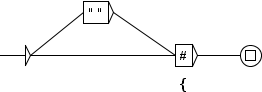
\includegraphics[width=262px]{resources/img/B.png}
\caption{Graphe B\label{fig-graphe-B}}
\end{center}
\end{figure}

Si on place des accolades ouvrantes et fermantes pour créer des étiquettes lexicales, il est possible de vérifier si, à partir d'un graphe, toutes les accolades ouvrantes sont bien fermées sur tous le chemins possibles. Pour cela il faut choisir dans le menu \textit{Graphs} la commande \textit{Tools/Verify braces} qui prend en compte l'appel à des sous-graphes B, BB, etc. Cependant cette vérification exige que les accolades soient ouvertes et fermées dans le même graphe. Par contre, ce programme vérifie aussi les sous-graphes appelés. Il compile en même temps le graphe examiné.


%%%%%%%%%%%%%%
\bigskip
\noindent \textbf{Poids}
\index{Poids}

\noindent On peut attribuer un poids à des boîtes d'un transducteur. Ainsi, lorsqu'une séquence est
reconnue par plusieurs chemins avec des sorties différentes
(transducteur ambigu\index{Ambigu!transducteur}\index{Sortie d'un transducteur!ambiguïté}),
seul un chemin de poids maximal sera conservé.
Après un "Locate", la concordance ne comportera qu'une seule fois la séquence reconnue, et avec la
sortie appropiée (figure~\ref{fig-weights-in-graphs}).

\begin{figure}[!ht]
\begin{center}
\includegraphics[width=14.5cm]{resources/img/fig5-15b.png}
\caption{Poids dans les graphes \label{fig-weights-in-graphs}}
\end{center}
\end{figure}

\bigskip
\noindent Les poids sont des valeurs entières. Pour donner à une boite
le poids 1, on insère \verb+${1}$+ dans la sortie de la boite, comme dans \verb+<E>/${1}$+.

\bigskip
\noindent Le poids d'un chemin est le dernier poids trouvé en parcourant le chemin.
Un poids peut être nul, mais pas strictement négatif. Un chemin qui a un poids, même nul, a la priorité sur un chemin
sans poids.

\bigskip
\noindent Avec des poids, on peut définir une priorité entre des chemins qui reconnaissent
la même séquence. On ne peut pas définir une priorité entre deux séquences dont une est incluse
dans l'autre (cf. section~\ref{section-configuration-recherche}), ni entre des séquences qui
se chevauchent  (cf. section~\ref{section-priorite-gauche}).

\bigskip
\noindent Les poids ne sont valides qu'à l'intérieur du graphe, et non dans les sous-graphes ni les graphes appelants. 

%%%%%%%%%%%%%

\subsection{Variables d'entrée}
\label{section-using-variables}
\index{Graphe!variables}\index{Variable!d'entrée}\index{\verbt{\$}}
\index{Transducteur!avec variables}

Il est possible de sélectionner des parties du texte reconnu par une grammaire au moyen
de variables d'entrée. Pour associer une variable d'entrée \verb+var1+ à une partie d’une grammaire, on utilise
soit le bouton avec les parenthèses rouges dans la barre d'icônes au-dessus du graphe (section ~\ref{toolbar-commands}),
soit les symboles spéciaux \verb+$var1(+ et \verb+$var1)+. (Ces symboles définissent respectivement le début et
la fin de la zone à mémoriser. Créez deux boîtes contenant l’une \verb+$var1(+ et l’autre
\verb+$var1)+. Ces boîtes ne doivent rien contenir d’autre que le nom de la variable précédé de
 \verb+$+ et suivi d’une parenthèse. Reliez ensuite ces boîtes à la zone de la grammaire voulue.)
 Dans le graphe de la figure~\ref{fig-using-variable}, on reconnaît une séquence commençant par
 un nombre, que l’on stocke dans une variable nommée \verb+var1+, suivi de \verb+dollar+ ou
 \verb+dollars+.

\begin{figure}[!ht]
\begin{center}
\includegraphics[width=13.5cm]{resources/img/fig5-16.png}
\caption{Utilisation d’une variable d'entrée
\texttt{var1}\label{fig-using-variable}}
\end{center}
\end{figure}

\bigskip
\noindent Les noms de variables peuvent contenir des lettres latines non accentuées, minuscules
ou majuscules, ainsi que des chiffres et le caractère \verb+_+ (underscore).
\index{\verbc{_}}\index{Noms de variables} Unitex fait la différence entre les lettres minuscules
et majuscules.\index{Underscore}

\bigskip
\noindent Quand une variable a ainsi été définie, on peut l’utiliser dans les sorties en encadrant
son nom avec le caractère \verb+$+.\index{\verbt{\$}} La grammaire de la
figure~\ref{fig-date-grammar} reconnaît une date formée d’un mois et d’une année,
 et produit en sortie la même date, mais dans l’ordre année-mois.

\bigskip
\noindent Si on veut utiliser le caractère \verb+$+ en sortie d'une boîte, on doit le
redoubler, comme le montre la figure~\ref{fig-using-variable}.

\begin{figure}[!ht]
\begin{center}
\includegraphics[width=14.5cm]{resources/img/fig5-17.png}
\caption{Interversion du mois et de l’année dans une date\label{fig-date-grammar}}
\end{center}
\end{figure}

\bigskip
\noindent Quand une boite redéfinit une variable qui avait déjà été définie,
\index{Variable!redéfinition} la nouvelle valeur écrase l'ancienne.
Ainsi, si la variable est définie dans une boucle, la valeur de la variable juste après
la boucle dépend du dernier passage dans la boucle.

\bigskip
\noindent Par défaut \verb+Locate+ et \verb+LocateTfst+ considèrent que les variables non définies
sont vides.\index{Variable!non définie}
On peut modifier ce comportement (voir section \ref{section-advanced-search-options}).
De plus, il est  possible dans un graphe d'interroger une variable pour savoir si elle a été initialisée ou non (section~\ref{section-variables}).

\subsection{Copie de listes}
\index{Copie!d'une liste}
\index{Copie}\index{Coller}

Il peut être pratique d’effectuer un copier-coller d’une liste de mots ou d’expressions
depuis un éditeur de texte vers une boîte dans un graphe. Afin d’éviter de devoir copier
manuellement chaque terme, Unitex propose un mécanisme de copie de listes. Pour l’utili-
ser, sélectionnez votre liste dans votre éditeur de texte et copiez-la au moyen de <Ctrl+C> ou
de la fonction de copie intégrée à votre éditeur. Créez ensuite une boîte dans votre graphe,
et utilisez <Ctrl+V> ou la commande "Paste" du menu "Edit" pour la coller dans la boîte.
Vous verrez alors apparaître la fenêtre de la figure~\ref{fig-setting-contexts-for-multiple-copy}.

\begin{figure}[!ht]
\begin{center}
\includegraphics[width=7cm]{resources/img/fig5-18.png}
\caption{Sélection de contexte pour la copie d’une
liste\label{fig-setting-contexts-for-multiple-copy}}
\end{center}
\end{figure}
\index{Contexte!copie de liste}

\bigskip
\noindent Cette fenêtre vous permet de définir les contextes gauche et droit qui seront ajoutés
automatiquement à chaque terme de la liste. Par défaut, ces contextes sont vides. Si l’on applique
les contextes \verb+<+ et \verb+.V>+ à la liste suivante:

\medskip
\textit{eat}

\textit{sleep}

\textit{drink}

\textit{play}

\textit{read}

\medskip
\noindent on obtient la boîte de la figure~\ref{fig-multiple-copy}.

\begin{figure}[!ht]
\begin{center}
\includegraphics[width=6.7cm]{resources/img/fig5-19.png}
\caption{Boîte obtenue par copie d’une liste avec ajout de contextes\label{fig-multiple-copy}}
\end{center}
\end{figure}

\subsection{Symboles spéciaux}
\index{Symboles!spéciaux}
\noindent L’éditeur de graphes d’Unitex interprète de façon particulière les symboles suivants:

\medskip
\verb," + : / < > # \,

\medskip
\noindent Le tableau ~\ref{tab-special-symbols} résume la signification pour Unitex de ces symboles,
ainsi que la ou les façons de reconnaître ces caractères dans des textes.

\index{Caractères spéciaux}
\begin{table}[!ht]
\begin{center}
\begin{tabular}{|c|p{9cm}|c|}
\hline
\texttt{Caractère} & \texttt{Signification} & \texttt{Codage}
\\
\hline \verb$"$ & les guillemets délimitent des séquences qui ne doivent
ni être interprétées par Unitex, ni subir de variantes de casse
& \verb$\"$
\\
\hline
\verb$+$ & \verb$+$ sépare les différentes lignes boîtes& \verb$"+"$
\\
\hline
\verb$:$ & \verb$:$ sert à introduire à appel à un sous-graphe& \verb$":"$ or \verb$\:$
\\
\hline
\verb$/$ & \verb$/$ indique le début de la sortie d'une boîte& \verb$\/$
\\
\hline
\verb$<$ & \verb$<$ indique le début d'un motif ou d'un méta& \verb$"<"$ or \verb$\<$
\\
\hline
\verb$>$ & \verb$>$ indique la fin d'un motif ou d'un méta& \verb$">"$ or \verb$\>$
\\
\hline
\verb$#$ & \verb$#$ sert à interdire la présence de l'espace& \verb$"#"$
\\
\hline
\verb$\$ & \verb$\$ sert à déspécialiser la plupart des caractères spéciaux& \verb$\\$
\\
\hline
\end{tabular}
\caption{Codage des symboles spéciaux dans l’éditeur de graphes\label{tab-special-symbols}}
\end{center}
\end{table}

\subsection{Commandes de la barre d’icônes}
\index{Barre d'outils}
\label{toolbar-commands}

La barre d’icônes présente au-dessus des graphes contient des raccourcis vers certaines
commandes et permet de manipuler les boîtes d’un graphe en utilisant des "outils". Cette
barre d’icônes peut être déplacée en cliquant sur la zone "rugueuse". Elle peut même être
dissociée du graphe et apparaître alors comme une fenêtre séparée (voir figure~\ref{fig-toolbar}).
Dans ce cas, le fait de fermer cette fenêtre replace la barre d’icônes à sa position initiale.
Chaque graphe possède sa propre barre d’icônes.

\begin{figure}[!ht]
\begin{center}
\includegraphics[width=15cm]{resources/img/fig5-20.png}
\caption{Barre d'outils\label{fig-toolbar}}
\end{center}
\end{figure}
\index{Copie}\index{Couper}\index{Coller}

\bigskip
\noindent Les deux premières icônes sont des raccourcis permettant de sauver et de compiler le
graphe. Les cinq suivantes correspondent aux opérations "Copier", "Couper", "Coller", "Redo" et
"Undo".

\bigskip
\noindent Les 6 icônes suivantes correspondent à des commandes d’édition des boîtes. La première,
en forme de flèche blanche, correspond au mode d’édition normal des boîtes. Les 5 autres
correspondent à des outils. Pour utiliser un outil, cliquez sur l’icône correspondante : le
curseur de la souris changera alors de forme et les clics de la souris seront alors interprétés
de façon particulière. Voici la description des outils, de gauche à droite:

\begin{itemize}
  \item création de boîtes: crée une boîte vide à l’endroit du clic;
  \item suppression de boîtes: supprime la boîte sur laquelle vous cliquez;
  \item relier des boîtes à une autre boîte: cet outil permet de sélectionner une ou plusieurs
boîtes, et de la ou les relier à une autre. À la différence du mode normal, la ou les
transitions qui vont être créées sont affichées pendant le déplacement du pointeur de
la souris;
  \item relier des boîtes à une autre boîte en sens inverse: cet outil effectue la même chose que
le précédent, mais en reliant en sens inverse les boîtes sélectionnées à la boîte cliquée;
  \item ouvrir un sous-graphe: ouvre un sous-graphe lorsque vous cliquez sur la ligne grisée
correspondante dans une boîte.
\end{itemize}

\noindent Pour que le curseur retrouve sa forme initiale de flèche blanche, faites un clic droit sur le fond du graphe~:
les clics seront à nouveau interprétés normalement.

\bigskip
\noindent L'icône en forme de clé anglaise est un raccourci pour ouvrir la fenêtre des options d'affichage
du graphe. Les deux suivantes permettent de voir les listes de graphes en relation avec le
graphe courant:

\begin{itemize}
\item Le premier bouton affiche la liste des graphes appelés par le graphe courant
\item Le deuxième bouton affiche la liste des graphes qui appellent le graphe courant
\end{itemize}

\noindent Le bouton muni de deux flèches vertes rafraîchit le graphe courant en chargeant sa dernière version.
Si un fichier \verb+.grf+ est modifié alors que le graphe qu'il contient est affiché dans
une fenêtre Unitex, une fenêtre pop up vous invitera à le recharger.

\bigskip
\noindent Le bouton portant l'icône d'une balance permet de comparer le graphe courant à un autre
graphe ou à une autre version du même graphe. Une nouvelle fenêtre est alors affichée (voir
	figure~\ref{Graph-DIFF}) qui contient les deux graphes avec des couleurs qui indiquent les types de différences entre les deux graphes : insertion, suppression,
déplacement de boîtes et changement de contenu d'une boîte apparaissent respectivement en vert,
rouge, mauve et jaune.

\begin{figure}[!ht]
\begin{center}
\includegraphics[width=15.6cm]{resources/img/DIFF.png}
\caption{DIFF\label{Graph-DIFF}}
\end{center}
\end{figure}

\bigskip
\noindent
Les six derniers boutons sont des raccourcis pour la définition d'une variable, du mode morphologique
ou d'un contexte sur une ou plusieurs boîtes sélectionnées. Ces boutons ne sont activés que si une  ou plusieurs boîtes sont sélectionnées:
\begin{itemize}
\item \textcolor{red}{()}  : variable d'entrée	(voir section~\ref{section-using-variables})
\item \textcolor{blue}{()} : variable de sortie (voir section~\ref{section-output-variables})
\item \textcolor{magenta}{<>} : mode morphologique (voir section~\ref{section-morphological-mode})
\item \textcolor{green}{\$*} : contexte gauche (voir section~\ref{section-contexts})
\item \textcolor{green}{\$[} : contexte droit (voir section~\ref{section-contexts})
\item \textcolor{green}{\$![} : contexte droit négatif (voir section~\ref{section-contexts})
\end{itemize}

%\pagebreak


%%%%%%%%%%%%%%%%%%%

\section{Options de présentation}
\index{Graphe!présentation}

\subsection{Tri des lignes d’une boîte}
\index{Tri!des lignes d'une boîte}\index{Boîtes!tri des lignes}
Vous pouvez trier le contenu d’une boîte en la sélectionnant et en cliquant sur "Sort Node
Label" dans le sous-menu "Tools" du menu "FSGraph". Ce tri ne fait pas appel au programme
\verb+SortTxt+. Il s’agit d’un tri basique qui trie les lignes de la boîte selon l’ordre des
caractères dans le codage Unicode.\index{Unicode}


\subsection{Zoom}
\index{Zoom}\index{Graphe!zoom}
Le sous-menu "Zoom" vous permet de choisir l’échelle à laquelle sera affiché le graphe.

\bigskip
\begin{figure}[!ht]
\begin{center}
\includegraphics[width=6.4cm]{resources/img/fig5-21.png}
\caption{Sous-menu Zoom}
\end{center}
\end{figure}

\noindent L’option "Fit in screen" étire ou rétrécit le graphe pour lui donner la taille de l’écran.
L’option "Fit in window" ajuste le graphe pour qu’il soit entièrement affiché dans la fenêtre.


\subsection{Antialiasing}
\index{Antialiasing}\index{Graphe!antialiasing}
L’antialiasing est un effet de rendu qui permet d’éviter l’effet de pixellisation.
\index{Pixellisation} Vous pouvez activer cet effet en cliquant sur "Antialiasing..."
dans le sous-menu "Format". La figure~\ref{fig-antialiasing} montre deux graphes affichés
normalement (graphe du haut) et avec antialiasing (graphe du bas).


\bigskip
\begin{figure}[!ht]
\begin{center}
\includegraphics[width=13.5cm]{resources/img/fig5-22.png}
\caption{Exemple d'antialiasing\label{fig-antialiasing}}
\end{center}
\end{figure}

\noindent Cet effet ralentit l’exécution d’Unitex. Nous vous conseillons de ne pas l’utiliser
si votre machine est peu puissante.


%\clearpage

\subsection{Alignement des boîtes}\index{Boîtes!alignement}
\index{Alignement des boîtes}\index{Graphe!alignement des boîtes}
Afin d’obtenir des graphes harmonieux, il est utile de pouvoir aligner les boîtes, aussi
bien horizontalement que verticalement. Pour cela, sélectionnez les boîtes à aligner et cli-
quez sur "Alignment..." dans le sous-menu "Format" du menu "FSGraph" ou appuyez sur
<Ctrl+M>. Vous voyez alors apparaître la fenêtre de la figure~\ref{fig-alignment-frame}.

\bigskip
\noindent Les possibilités d’alignement horizontal sont:
\begin{itemize}
  \item Top: les boîtes sont alignées sur la boîte la plus haute;
  \item Center: les boîtes sont toutes centrées sur un même axe;
  \item Bottom: les boîtes sont alignées sur la boîte la plus basse.
\end{itemize}

\begin{figure}[!ht]
\begin{center}
\includegraphics[width=6.6cm]{resources/img/fig5-23.png}
\caption{Fenêtre d’alignement\label{fig-alignment-frame}}
\end{center}
\end{figure}

\noindent Les possibilités d’alignement vertical sont:
\begin{itemize}
  \item Left: les boîtes sont alignées sur la boîte la plus à gauche;
  \item Center: les boîtes sont toutes centrées sur un même axe;
  \item Right: les boîtes sont alignées sur la boîte la plus à droite.
\end{itemize}

\bigskip
\noindent La figure ~\ref{fig-vertical-left-alignment} montre un exemple 
d’alignement. Le groupe de boîtes situé à droite est une copie des boîtes
de gauche qui a été alignée verticalement à gauche.


\bigskip
\begin{figure}[!ht]
\begin{center}
\includegraphics[width=11.5cm]{resources/img/fig5-24.png}
\caption{Exemple d’alignement vertical gauche\label{fig-vertical-left-alignment}}
\end{center}
\end{figure}

\bigskip
\noindent L’option "Use Grid" de la fenêtre d’alignement permet d’afficher une grille en
arrière-plan du graphe. Cela permet d’aligner approximativement les boîtes.
\index{Grille}

\bigskip
\begin{figure}[!ht]
\begin{center}
\includegraphics[width=15cm]{resources/img/fig5-25.png}
\caption{Exemple d’utilisation d’une grille}
\end{center}
\end{figure}

\subsection{Présentation, polices et couleurs}
\label{section-display-fonts-colors}
\index{Graphe!options d'affichage, polices et couleurs}\index{Options!configuration}
\index{Couleurs!configuration}
Vous pouvez configurer l’aspect d’un graphe en appuyant sur <Ctrl+R> ou en cliquant
sur "Presentation..." dans le sous-menu "Format" du menu "FSGraph", ce qui provoque l’af-
fichage de la fenêtre de la figure~\ref{fig-graph-display-configuration}.

\begin{figure}[!ht]
\begin{center}
\includegraphics[width=9cm]{resources/img/fig5-26.png}
\caption{Configuration de l’aspect d’un graphe\label{fig-graph-display-configuration}}
\end{center}
\end{figure}

\bigskip
\noindent Les paramètres de polices sont:
\begin{itemize}
  \item Input: police utilisée dans les boîtes, ainsi que dans la zone de texte où l’on édite le
contenu des boîtes;
\item Output: police utilisée pour afficher les sorties des boîtes.\index{Sortie d'un transducteur}
\end{itemize}

\bigskip
\noindent Les paramètres de couleur sont:
\begin{itemize}
  \item Background: couleur de fond;
  \item Foreground: couleur utilisée pour le texte et le dessin des boîtes;
  \item Auxiliary Nodes: couleur des boîtes faisant appel à des sous-graphes ;
  \item Selected Nodes: couleur utilisée pour dessiner les boîtes quand elles sont sélectionnées ;
  \item Comment Nodes: couleur utilisée pour dessiner les boîtes qui ne sont reliées à aucune autre.
\end{itemize}

\bigskip
\noindent Les autres paramètres sont:
\begin{itemize}
  \item Date: affichage de la date courante dans le coin inférieur gauche du graphe;
  \item File Name: affichage du nom du graphe dans le coin inférieur gauche du graphe;
  \item Pathname: affichage du nom du graphe avec son chemin complet dans le coin inférieur
gauche du graphe. Cette option n’a d’effet que si l’option "File Name" est sélectionnée;
  \item Frame: dessine un cadre autour du graphe;
  \item Right to Left: inverse le sens de lecture du graphe (voir exemple de la
  		  figure~\ref{fig-right-to-left-graph}).
\end{itemize}

\bigskip
\begin{figure}[!ht]
\begin{center}
\includegraphics[width=14.5cm]{resources/img/fig5-27.png}
\caption{Graphe se lisant de droite à gauche\label{fig-right-to-left-graph}}
\end{center}
\end{figure}

\bigskip
\noindent Vous pouvez rétablir les paramètres par défaut en cliquant sur le bouton "Default".
Si vous cliquez sur le bouton "OK", seul le graphe courant sera modifié.\index{Préférences}
Pour modifier les préférences par défaut d’une langue, cliquez sur "Preferences..." dans le
menu "Info" et choisissez l’onglet "Graph Presentation".

%La fenêtre de configuration des préférences possède
%une option supplémentaire concernant l’antialiasing (voir figure
%order to modify the preferences for a language as a default, click on
%"Preferences..." in the "Info" menu and click on the "Graph configuration" button 
%in the "Language \& Presentation" tab.


\section{Les graphes en dehors d’Unitex}
\label{exporting-graphs}
\subsection{Inclusion d’un graphe dans un document}
\index{Graphe!inclure dans un document}\index{Inclure un graphe dans un document}
\index{Graphe!export en PNG}
Pour inclure un graphe dans un document, il faut en faire une image. Pour cela, une
première méthode consiste à exporter votre graphe vers un format d'image~: PNG, JPEG ou SVG. Pour
cela, allez dans le menu "FSGraph" et cliquez sur "Export as image". Choisissez ensuite le type de
fichier. Vous obtiendrez ainsi une image prête à être intégrée dans un document ou
à être éditée avec un logiciel de retouche d’images. Afin de rendre l’image plus lisse, vous
pouvez activer l’antialiasing pour le graphe qui vous intéresse. Contraitement au JPEG, le format PNG
utilise une compression sans perte de qualité, donc le PNG donne toujours un meilleurs résultat que le
JPEG. Et contrairement au PNG et au JPEG, qui sont des fomats bitmap, le
format SVG est un format vectoriel, ce qui permet souvent un meilleur résultat. A l'aide du logiciel Inkscape, il
est également possible de convertir le fichier SVG en EPS ou en PDF, avec des lignes de commandes de ce type:
\begin{verbatim}
Inkscape -z -E graph.eps graph.svg
\end{verbatim}
\begin{verbatim}
Inkscape -z -A graph.pdf graph.svg
\end{verbatim}

\bigskip
\noindent La seconde méthode consiste à faire une capture d’écran:

\bigskip
\noindent Sous Windows:

\bigskip
\noindent Appuyez sur la touche "Imprime écran" de votre clavier qui doit se trouver près
de la touche F12. Lancez le programme \verb+Paint+ dans le menu "Accessoires" de Windows. Appuyez sur 
<Ctrl+V>. \verb+Paint+ peut vous dire que l’image contenue dans le presse-papiers
est trop grande et vous demander si vous voulez agrandir l’image. Cliquez sur "Oui". Vous
pouvez maintenant éditer l’image de l’écran. Sélectionnez la zone qui vous intéresse. Pour
cela, passez en mode sélection en cliquant sur le rectangle en pointillé qui se trouve dans
le coin supérieur gauche de la fenêtre. Vous pouvez maintenant sélectionner une zone de
l’image avec la souris. Une fois votre zone sélectionnée, appuyez sur <Ctrl+C>. Votre sélection
est maintenant dans le presse-papier, il ne vous reste plus qu’à aller dans votre document
et à appuyer sur <Ctrl+V> pour coller votre image.


\bigskip
\noindent Sous Linux:

\bigskip
\noindent Effectuez une capture d’écran (par exemple avec le programme \verb+xv+). Retaillez ensuite
votre image avec un éditeur graphique (par exemple \verb+TheGimp+), et collez votre image dans
votre document de la même façon que sous Windows.

\bigskip
\noindent\textbf{Image vectorielle}
\index{SVG export de graphe}
\index{Graphe!export en SVG}

\bigskip
\noindent Si vous préférez une image vectorielle, vous pouvez exporter votre graphe vers le format
SVG, qui est utilisable avec des logiciels comme Inkscape (\cite{Inkscape}).
Il permet d'obtenir des sorties PostScript utilisables dans des documents \LaTeX.

\subsection{Impression d’un graphe}
\index{Impression!d’un graphe}

Vous pouvez imprimer un graphe en cliquant sur "Print..." dans le menu "FSGraph" ou
en appuyant sur <Ctrl+P>.


\bigskip
\noindent ATTENTION: vous devez vous assurer que le paramètre d’orientation de l’imprimante
(portrait ou paysage) correspond bien à l’orientation de votre graphe.


\bigskip
\noindent Vous pouvez définir vos préférences d’impression en cliquant sur "Page Setup" dans le
menu "FSGraph". Vous pouvez également imprimer tous les graphes qui sont ouverts en
cliquant sur "Print All...".




\input{06-advanced-use_FR_utf8}
\input{07-text_automaton_FR_utf8}
\input{08-sequence-automaton_FR_utf8}
\input{09-lexicon-grammar_FR_utf8}
\input{10-alignment_FR_utf8}
\input{11-multiflex_FR_utf8}
\chapter{Cascade de Transducteurs}
\label{chap-cassys}

Ce chapitre presente l'outil \textit{CasSys} qui donne la possibilité de créer une cascade
de  transducteurs et de nouvelles manières de travailler sur la langue naturelle avec des 
graphes à états finis. Une \textit{cascade de transducteurs} \index{cascade de transducteurs}
applique plusieurs graphes (automates ou transducteurs), l'un après l'autre, sur le texte: chaque
graphe modifie le texte, et les changements peuvent être utilisés pour des traitements supplémentaires
par les graphes suivants. Ce type de  système est notamment utilisé pour l'analyse syntaxique, le chunking,
l'extraction d'information, la reconnaissance d'entitiés nommées etc. Pour faire cela, CasSys utilise
une succession de "locate patterns" avec les options adéquates.

\bigskip
\noindent Le premier prototype du système \textit{CasSys} \index{CasSys}  a été créé en 2002 au 
laboratoire LI (Laboratoire d'Informatique de l'Université de Tours) (\cite{these-nathalie}). 
Ce prototype était entièrement spécialisé pour l'extraction d'entités nommées. CasSys a été  
ensuite généralisé pour effectuer n'importe quelle sorte de traitement nécessitant une cascade. 
Il a été constamment amélioré au cours des années, sans être réellement intégré à Unitex. 
C'est grâce à un projet récent \footnote{"Feder-Région Centre entités nommées et nommables" 
dirigé par Denis Maurel, LI, Tours, France, intégration réalisée par Nathalie Friburger et
David Nott}que l'intégration complète  de CasSys à Unitex a pu être réalisée.

Les grammaire Unitex sont de type Context free et intègrent la notion de transduction issue
du domaine des automates à états finis. Une grammaire avec transduction (un  transducteur) est
capable de produire une sortie. CasSys est spécialisé dans l'application de transducteurs sous
la forme d'une cascade.

\bigskip
Une cascade peut être utilisée pour l'analyse syntaxique, le chunking, l'extraction d'information, etc. 
\noindent Les transducteurs sont intéréssants car ils permettent d'associer à la séquence
reconnue l'information qui se trouve dans sorties des graphes.
Ces  sorties peuvent :
\begin{itemize}
\item Être ajoutées à la séquence reconnue et apparaître dans la concordance résultante ou le texte modifié.
\item Remplacer la séquence reconnue pour modifier le texte.
\end{itemize}
\noindent Ces deux  opérations transforment le texte ou lui ajoute des informations.

\bigskip
\noindent Dans ce chapitre, nous expliquons comment créer des cascades de transducteurs et
comment les appliquer. Ensuite, nous détaillons les options et possibilités offertent par CasSys.

%%%%%%%%%%%%%%%%%%%%%%%%%%%%%%%%%%%%%%%%%%%%%%%%%%%%%%%%%%%%%
\section{Appliquer une cascade de Transducteurs avec CasSys}
\label{section:applyCascade}
Appliquer une cascade de transducteurs avec CasSys consiste à représenter un phénomène linguistique par une
liste de transducteurs à appliquer au texte dans un ordre précis: CasSys et son interface dans Unitex permet d'y parvenir.
Cette section explique comment utiliser l'interface pour créer et gérer les graphes (ordre, ajout, suppression) et appliquer la cascade.   

%%%%%%%%%%%%
\subsection{Création de la liste des transducteurs}
\label{subsec:listTrans}

\bigskip
\noindent Afin de pouvoir gérer la liste de transducteur, le menu FSGraph comporte deux sous-menus:
"\textit{New cascade}" et "\textit{Edit cascade...}" (Figure \ref{fig13-08}). Pour créer la liste des
transducteurs, sélectionnez "\textit{New cascade}". Si vous souhaitez modifier une cascade existante, sélectionnez
"\textit{Edit cascade...}", puis  choisissez le nom de la cascade à ouvrir.

\begin{figure}[!htb]
 \centering
 \includegraphics[width=4cm]{resources/img/fig13-08.png}
 \caption{Menu "FSGraph" d'Unitex et sous-menu "New Cascade" et "\textit{Edit cascade...}"}
 \label{fig13-08}
\end{figure}

Le répertoire de la langue courante contient un sous-répertoire nommé CasSys dans lequel se trouvent
les fichiers de configuration d'une cascade. Ce sont des fichiers textes avec l'extension \textit{.csc} (ex: ma cascade.csc)

\subsection{Edition de la liste des transducteurs}
\label{subsec:editlistTrans}

La fenêtre de configuration de CasSys (\ref{fig13-03}) comporte trois parties :

\begin{figure}[!htb]
  \centering
  \includegraphics[width=16cm]{resources/img/fig13-03.png}
  \caption{Fenêtre de configuration de CasSys avec à droite la liste des transducteurs}
  \label{fig13-03}
\end{figure}

\begin{enumerate}
	\item Un \textit{gestionnaire de fichier} à gauche du cadre permet de choisir les transducteurs à mettre dans la cascade.
	Le gestionnaire n'affiche que les fichiers fst2 (tous les graphes que vous souhaitez mettre dans la liste doivent être compilés au format fst2).
	
	Pour éditer la cascade, choisissez les graphes à gauche et mettez les à droite à l'aide d'un glisser-déposer.
\item Le \textit{tableau} de droite affiche la cascade: la liste ordonnée des transducteurs et les options sélectionnées pour chaque graphe.
		Le tableau est évidemment vide pour une nouvelle cascade.
		 
		Les colonnes du tableau (Figure \ref{fig13-09}) donne le numéro de chaque graphe et permettent de choisir leur comportement.
	\begin{itemize}
	\item \textbf{\#} : Numéro du graphe/transducteur dans la cascade pour chaque graphe; le fichier fst2 est numéroté.
	\item \textbf{Disabled} : Pour désélectionner le graphe courant. \textit{Disabled} siginifie: "\textit{non appliqué dans la cascade}".
		Les graphes non sélectionnés apparaissent sans numéro, en grisé et barré.
	\item \textbf{Name} : Le nom du graphe (avec l'extension \emph{fst2}). Si vous laissez la souris sur le nom du graphe,
		une info-bulle apparaît avec le chemin complet du graphe.
		Les graphes dont le fichier source n'est pas trouvé apparaissent en italique et en rouge.

	\item \textbf{Merge}: Si le transducteur doit être appliqué en mode merge.
	\item \textbf{Replace}: Si le transducteur doit être appliqué en mode replace.
	\item \textbf{Until fix point}: Si le transducteur doit être appliqué une fois ou plusieurs fois
		jusqu'à ce que le texte soit inchangé c'est à dire qu'un point fixe est atteint (voir \ref{sub:AppWhiCon}).
	\end{itemize}
	
	 \item Au centre se trouvent les boutons décrits ci-dessous:
		\begin{itemize}
		\item \textit{"Up"/"Down"/"Top"/"Bottom"} sont utilisés pour modifier l'ordre
		des transducteurs dans la liste (ils déplacent le transducteur sélectionné); 
		\textit{"Up"} et \textit{"Down"} déplacent le transducteur sélectionné d'une ligne vers le haut ou
			vers le bas, \textit{"Top"} et \textit{"Bottom"} le positonnent au début ou à la fin de la liste.
		\item \textit{"Delete"} permet de supprimer le transducteur sélectionné de
		la liste des transducteurs. 
		\item \textit{"Add"} ajoute un transducteur (précédemment sélectionné) dans la liste.
			Il remplace le gisser-déposer préalablement décrit.
		\item \textit{"View"} ouvre le graphe sélectionné aussi bien dans l'explorateur
		de fichiers que dans la liste de transducteurs. Il est très utile d'avoir un accès
		rapide à n'importe quel transducteur aussi bien pour y jeter un coup d'œil que pour
		le modifier.
		\item \textit{"Save"} et \textit{"Save as"} permettent d'enregistrer la
		liste des transducteurs. Par défaut, les listes des transducteurs sont placées dans
		le répertoire CasSys de la langue courante  (par exemple French/CasSys).
		\item \textit{"Compile"} recompile tous les graphes de la cascade.	
		\item \textit{"Disable all"} pour désélectionner tous les graphes de la cascade.	
		\item \textit{"Enable all"} pour sélectionner tous les graphes de la cascade.	
		\item \textit{"Close"} ferme la fenêtre courante.
		\end{itemize}
\end{enumerate}


\begin{figure}[!htb]
  \centering
  \includegraphics[width=7cm]{resources/img/fig13-09.png}
  \caption{La table/liste de transducteurs}
  \label{fig13-09}
\end{figure}

	

\subsection{Application d'une cascade}
\label{subsec:launchCascade}

Dans le menu "Text", sélectionner le sous-menu "\textit{Apply CasSys cascade...}" (Figure \ref{fig13-01}) pour ouvrir la fenêtre CasSys.
Ce sous-menu "\textit{Apply CasSys cascade...}" n'est actif que si un texte a été préalablement ouvert.

\begin{figure}[!htb]
 \centering
 \includegraphics[width=5cm]{resources/img/fig13-01.png}
 \caption{Menu "Text" d'Unitex et sous-menu "Apply CasSys Cascade"}
 \label{fig13-01}
\end{figure}

La fenêtre CasSys (\ref{fig13-02}) affiche le contenu du répertoire CasSys de la langue courante. Elle
permet de choisir le fichier contenant la liste de transducteurs à appliquer au texte. Une fois que cette liste
est choisie, vous pouvez cliquer sur le bouton "Launch" pour appliquer la cascade.

\begin{figure}[!htb]
  \centering
  \includegraphics[width=10cm]{resources/img/fig13-02.png}
  \caption{Fenêtre de lancement de la cascade de transducteurs}
  \label{fig13-02}
\end{figure}

N'importe quel dictionnaire du mode morphologique déclaré dans vos préférences est utlisable dans vos
graphes.
Les  préférences peuvent être modifiées à partir du menu "Info" (Info -->
Preferences --> morphological-mode dictionaries).

\subsection{Partage d'un fichier liste de transducteurs en cascade}
\label{subsec:shareCascade}

Afin de faciliter le travail collaboratif avec CasSys, une fonctionnalité d'export/import est
fournie à l'aide d'un fichier liste de transducteurs. Cette possibilité est offerte par le menu
"\textit{Text / Apply CasSys cascade...}" (Figure \ref{fig13-02}).

Pour partager un fichier liste de cascade, les points suivants doivent être remplis:
\begin{enumerate}
\item \textbf{Export :} Choisissez un fichier cascade et cliquez sur le bouton "export".
	(Un fichier partageable est créé dans le répertoire \texttt{/CasSys/Share})
\item Envoyez le fichier partagé à vos collègues
\item \textbf{Import :} Choisissez un fichier  et cliquez sur le bouton "import".
	(Un fichier prêt à être utilisé est créé dans le répertoire \texttt{/CasSys})
\end{enumerate}

%%%%%%%%%%%%%%%%%%%%%%%%%%%%%%%%%%%%%%%%%%%%%%%%%%%%%%%
\section{CasSys en détail}

Dans cette section nous présentons une description détaillée du fonctionnement de CasSys.

\subsection{Type de graphe utilisé}
\label{graphs-for-cassys}

CasSys utilise la version compilée des graphes (format \verb+.fst2+). CasSys gère les grammaires locales
(section~\ref{syntactic-graphs}) présentées dans le chapitre \ref{chap-advanced-grammars}.
Les grammaires utilisées dans une cascade suivent les mêmes règles que les grammaires habituellement
utilisées dans Unitex. Elles peuvent comporter des sous-graphes, utiliser le mode morphologique et les filtres
morphologiques, et faire référence aux informations présentes dans les dictionnaires. 

\bigskip
\noindent CasSys n'est pas compatible avec les fichiers \verb+fst2+ en mode debug (\ref{section-debug-mode}).
Quand on applique un graphe en mode debug avec le menu \verb+Text>Locate Pattern+, le système
compile le graphe dans un format spécial de mode debug. Pour obtenir un fichier au format \verb+fst2+ normal,
recompilez le graphe, soit avec le menu \verb+FSGraph+, soit en ligne de commande, soit en décochant le mode
debug avant d'appliquer le graphe avec \verb+Locate Pattern+.

\subsection{Application itérative}
\label{sub:AppWhiCon}

CasSys peut appliquer un graphe sur un texte de manière itérative tant que de nouvelles concordances sont obtenues.
Ce comportement est sélectionné ou non pour chaque graphe selon que la case \verb+Until fix point+ est cochée ou non. Cette section présente le comportement de cette option\\

Considérons par exemple le graphe \ref{fig:AB->A} qui reconnait \emph{AB} et le remplace par \emph{A}.\\

\begin{figure}[!htbp]
  \centering
  \includegraphics[width=6cm]{resources/img/AB_to_A.png}
  \caption{Transducteur qui modifie BA en A}
  \label{fig:AB->A}
\end{figure}

Considérons le texte \emph{B B B A A A}. L'application du graphe \ref{fig:AB->A} sur ce texte avec \emph{Until fix point}  donne :\\

\begin{tabular}{|l|cccccc|r|}
\hline
initial text  &B&B&B&A&A&A&\\
\hline
itération 1 & &B&B&A&A&A& 1 match\\
itération 2 & & &B&A&A&A& 1 match\\
itération 3 & & & &A&A&A& 1 match\\
itération 4 & & & &A&A&A& 0 match\\
\hline
\end{tabular}

\bigskip
Durant les trois premières itérations, une concordance est obtenue, le graphe
est alors appliqué à nouveau au texte résultant. A la quatrième itération, aucune
concordance n'est trouvée, le graphe n'est donc plus réappliqué.

\bigskip
\large{\textbf{Attention :}} Prendre garde à la possibilité de blocage en utilisant cette 
option. Par exemple, un transducteur qui reconnaît \emph{A} et le remplace par
\emph{A} causerait un blocage s'il était appliqué sur le texte de l'exemple.

\begin{comment}
\subsection{Un texte au format de type XML avec étiquettes lexicales}

En sortie, le format avec étiquettes lexicales est transformé en un format de type XML.
Ce changement est fait dans le but de proposer un texte plus manipulable  à l'utilisateur final.

A partir de ce format, il est plus facile d'obtenir une sortie adaptable à tous.\\

Plus précisement, les étiquettes lexicales :\\
\begin{tabular}{c}
\texttt{
\{forme.lemme,code1+code2:flex1:flex2\}}
\end{tabular}\\

La sortie CaSsys de type XML a le format suivant :\\
\begin{tabular}{ll}
\texttt{<csc>}&\\
	&\texttt{<form>forme</form>}\\
	&\texttt{<lem>lemme</lem>}\\
	&\texttt{<code>code1</code>}\\
	&\texttt{<code>code2</code>}\\
	&\texttt{<inflect>flex1</inflect>}\\
	&\texttt{<inflect>flex2</inflect>}\\
\texttt{</csc>}&\\
\end{tabular}
\end{comment}


\subsection{Règles utilisées dans une cascade}

Dans une cascade, chaque graphe observe les règles utilisées dans Unitex:
\begin{itemize}
	\item Insertion à gauche des motifs reconnus : en mode "merge", la sortie est insérée à
	gauche de la séquence reconnue.
	\item	Priorité au motif le plus à gauche : lors de l'application d'une grammaire locale,
	les occurrences qui se chevauchent sont toutes indexées. 
	Durant la construction de la concordance, toutes ces occurrences sont présentes, mais comme CasSys
	modifie le texte après application de chaque 
	graphe de la cascade, il est nécessaire de choisir parmi ces occurrences celle à prendre en
	compte. La priorité est donnée à la séquence la plus à gauche.
	\item Priorité au plus long motif: dans CasSys, lors de l'application d'un graphe, c'est la
	séquence la plus longue qui est conservée.
	\item	Limitation du nombre d'occurrences recherchées: dans CasSys, ce nombre n'est pas
	limité : une telle limitation n'a aucun sens dans CasSys. Toutes les occurrences sont
	toujours indexées dans le texte.
\end{itemize}

\subsection{Marquage de motifs dans CasSys}

La sortie des transducteurs peut être utilisée pour insérer des informations dans les textes, en
particulier pour marquer les motifs reconnus: il est possible d'utiliser toute sorte de marques, 
( ), [], "", etc. ou des balises xml comme <xxx> </xxx>, mais CasSys propose une manière
particulière d'annoter les motifs reconnus, offrant certaines possibilités que nous présentons
maintenant.  

\bigskip
\noindent Unitex découpe les textes en tokens de différentes sortes comme le marqueur de fin de
phrase {S}; le marqueur {STOP}, des séquences de lettres contiguës, des étiquettes lexicales
{aujourd'hui,.ADV}, etc. Les étiquettes lexicales sont utilisées dans CasSys de manière
particulière. Une étiquette lexicale (entre accolades) est habituellement utilisée pour éviter les
ambiguïtés (voir les explications à la section \ref{tokenization} et à la section
\ref{section-displaying-sentence-automata}). 
Par exemple, dans un texte, si vous avez le token \emph{\{curly brackets,.N\}}, ni "curly" ni
"brackets" ne seront reconnus, mais seulement la séquence toute entière
"curly brackets". Une étiquette lexicale peut contenir une information lexicale complexe comme
\emph{N+Pers+Hum:fs}.
Dans un graphe, il est possible de chercher un token en utilisant l'information contenue dans un
masque lexical : par exemple, on peut écrire \emph{<.N>} pour chercher 
un nom, \emph{<.Pers+Hum>} pour un être humain ou \emph{<.Pers>}. Ces masques lexicaux sont décrits
dans le chapitre "Recherche d'expressions rationnelles" section
\ref{section-special-symbols}.
 
\bigskip
\noindent Dans CasSys, nous utilisons la marque lexicale de manière particulière. Une cascade de
transducteurs est intéressante pour localiser un îlot de certitude. Il est nécessaire pour ce type
de système d'éviter que des motifs précédemment reconnus soient ambigus avec ceux reconnus par les
graphes suivants. Pour éviter cela, on étiquette les motifs reconnus par les graphes sous la forme
\emph{\{} et \emph{,.tag1+tag2+tagn\}} (où \emph{tag1, tag2, etc.} sont vos propres étiquettes).

\bigskip
\noindent Pour expliciter ce comportement, voici un exemple très simple. Le texte sur lequel nous
travaillons est :

\emph{bac a b c cc a b b ba ab a b bca a b c abaabc}.

\bigskip
\noindent Le graphe grfAB (\ref{fig13-05}) reconnaît la séquence \emph{ab} dans le texte et lui
ajoute l'étiquette lexicale \{a b,.AB\}. Ce graphe appliqué en mode MERGE ajoute \emph{\{ } et
 \emph{,.AB\}} dans le texte.

\begin{figure}[!htb]
  \centering
  \includegraphics[width=6cm]{resources/img/fig13-05.png}
  \caption{Le graphe grfAB}
  \label{fig13-05}
\end{figure}

\bigskip
\noindent Le texte résultant est : \emph{bac \{a b,.AB\} c cc \{a b,.AB\} b ba ab \{a b,.AB\} bca
\{a b,.AB\} c abaabc}.

\bigskip
\noindent Maintenant le motif \emph{a b} est étiqueté \emph{AB}. La partie (a ou b seul) de ce
motif ne peut pas l'être à cause de l'étiquetage de \emph{a b}.

\bigskip
\noindent Après ce graphe, la cascade applique un autre graphe nommé "tagAB" (\ref{fig13-06})
contenant le masque lexical <AB>. Il reconnait toutes les séquences lexicalement étiquetées par le
graphe précédent.

\begin{figure}[!htb]
  \centering
  \includegraphics[width=10cm]{resources/img/fig13-06.png}
  \caption{Le graphe tagAB}
  \label{fig13-06}
\end{figure}

\bigskip
\noindent Le texte résultant est : \emph{bac \{\{a b,.AB\} c,.ABC\} cc \{a b,.AB\} b ba ab \{a
b,.AB\} \{bca,.BCA\} \{\{a b,.AB\} c,.ABC\} abaabc}.


\bigskip
\noindent La concordance affichée par Unitex devrait ressembler à celle de la figure
(\ref{fig13-07}). Pour des raisons liées à la programmation (les ambiguïtés entre les
	caractères entre accolades des étiquettes lexicales), nous n'avons d'autres options que de
placer des  $\backslash$ avant chaque caractère ambigu; c'est pourquoi ces symboles sont précédés de
$\backslash$ dans la concordance pour éviter des problèmes avec Unitex.

\begin{figure}[!htb]
  \centering
  \includegraphics[width=15cm]{resources/img/fig13-07.png}
  \caption{La concordance issue l'application de la cascade}
  \label{fig13-07}
\end{figure}

\section{Graphes de g\'{e}n\'{e}ralisation d'\'{e}tiquetage}

Parfois, on a identifi\'{e} des \'{e}l\'{e}ments recherch\'{e}s gr\^{a}ce \`{a} leur contexte, mais si ces \'{e}l\'{e}ments apparaissent ailleurs hors contexte on ne les reconna\^{i}t pas. Afin de trouver de telles occurences, CasSys propose d'utiliser des graphes de g\'{e}n\'{e}ralisation d'\'{e}tiquetage. Ces graphes contiennent des bo\^{i}tes vides qui sont remplies automatiquement par le programme avant d'\^{e}tre appliqu\'{e}s au texte. Ces graphes de g\'{e}n\'{e}ralisation d'\'{e}tiquetage ne fonctionnent qu'avec l'utilisation d'accolades, car le programme consulte la liste de tokens (tokens.txt) du texte \`{a} analyser par le futur graphe.

Dans le cas d'un token comme :

\emph{\{\{mars,.mois\} \{2018,.année\},.date\}}

nous appellerons dans la \emph{suite sous-étiquette lexicale} les éléments \emph{\{mars,.mois\}} et \emph{\{2018,.année\}}, et \emph{sous-catégorie} les catégories \textit{mois} et \textit{année}.

\subsection{D\'{e}claration d'un graphe de g\'{e}n\'{e}ralisation d'\'{e}tiquetage}
Pour que CasSys reconnaisse un graphe de g\'{e}n\'{e}ralisation d'\'{e}tiquetage il faut cocher la colonne \emph{Generalization} (figure \ref{fig12-3}).
\begin{figure}[!htb]
  \centering
  \includegraphics[width=15cm]{resources/img/fig12-3.png}
  \caption{Graphe de g\'{e}n\'{e}ralisation d'\'{e}tiquetage}
  \label{fig12-3}
\end{figure}

\subsection{Structure d'un graphe de g\'{e}n\'{e}ralisation d'\'{e}tiquetage}

\subsubsection{Graphe de généralisation d'étiquetage simple}

Pour créer un graphe de généralisation d'étiquetage, il faut marquer le début de la partie générique par une boîte \$G, avec en sortie une accolade ouvrante, et la fin par une boîte vide, avec en sortie une accolade fermante, éventuellement précédée d'un ou plusieurs traits. Il faut placer entre les deux une (et une seule) boîte vide avec en sortie l'élément à rechercher, précédé de ",.".

\bigskip
Il est possible d'utiliser le bouton \$G (figure~\ref{fig:bouton_g}) pour insérer automatiquement les boîtes de début et de fin de la partie générique après avoir sélectionné une boîte.

\begin{figure}[!htb]
  \centering
  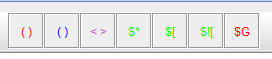
\includegraphics[width=8cm]{resources/img/bouton_g.png}
  \caption{Bouton \$G}
  \label{fig:bouton_g}
\end{figure}

\bigskip
Par exemple, si le fichier de tokens contient l'étiquette lexicale \emph{\{A,.x\}}, le graphe générique de la figure~\ref{fig:graphe_generique_simple} qui permet d'extraire les éléments de catégorie \textit{x} va générer le graphe en figure~\ref{fig:graphe_generique_simple_genere}. Un contexte droit négatif est ajouté automatiquement pour empêcher un deuxième étiquetage des occurrences déjà étiquetées.

\begin{figure}[!htb]
  \centering
  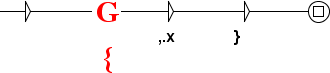
\includegraphics[width=8cm]{resources/img/graphe_generique_simple.png}
  \caption{Graphe de généralisation d'étiquetage simple}
  \label{fig:graphe_generique_simple}
\end{figure}

\begin{figure}[!htb]
  \centering
  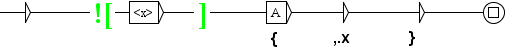
\includegraphics[width=10cm]{resources/img/graphe_generique_simple_genere.png}
  \caption{Graphe de généralisation d'étiquetage simple généré}
  \label{fig:graphe_generique_simple_genere}
\end{figure}

\bigskip
Remarque : Lors de la création d'un graphe de généralisation d'étiquetage, plusieurs parties génériques peuvent être insérées dans le graphe et des boîtes classiques peuvent être ajoutées avant et après chaque partie générique, comme le montre la figure~\ref{fig:graphe_generique_plusieurs_chemins}.

\begin{figure}[!htb]
  \centering
  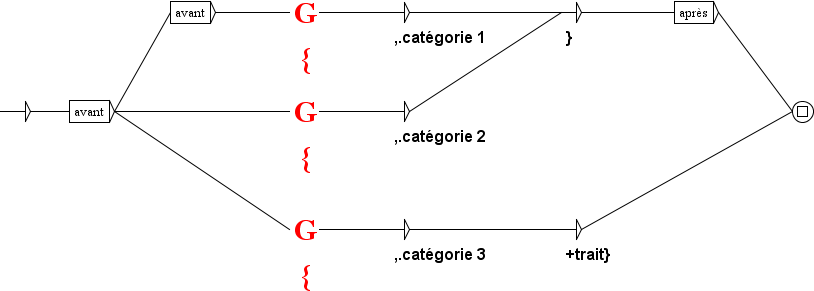
\includegraphics[width=14cm]{resources/img/graphe_generique_plusieurs_chemins.png}
  \caption{Graphe de généralisation d'étiquetage avec plusieurs chemins}
  \label{fig:graphe_generique_plusieurs_chemins}
\end{figure}

\subsubsection{Graphe de généralisation d'étiquetage avec restriction\protect\footnote{Dans certaines versions 3.2 alpha des restrictions négatives étaient présentes. Elles ne le sont plus, mais le comportement d'une partie générique utilisant des restrictions négatives peut être reproduit en utilisant des restrictions positives. Pour plus d'information ou en cas de besoin, contacter la liste Google Unitex.}}

Les graphes simples permettent de récupérer le contenu des tokens de catégorie cherchée du fichier tokens.txt, mais il peut arriver que l'on veuille récupérer le contenu d'une sous-étiquette lexicale. Pour cela on peut utiliser des restrictions dans les graphes de généralisation d'étiquetage. On place alors la sous-catégorie à rechercher dans la boîte, tout en laissant en sortie la catégorie principale précédée de ",.". Cette sous-catégorie doit être seul dans la boîte. Si on veut extraire plusieurs sous-catégories il faut créer plusieurs chemins.


\bigskip
Prenons un exemple, supposons que la ligne suivante soit présente dans le fichier tokens.txt :


\emph{\{\{premier,.A\} \{\{deuxième,.A\} \{troisième,.B\},.B\},.principal\}}

et que l'on veuille extraire la sous-étiquette lexicale de sous-catégorie \textit{A} ou celle de sous-catégorie \textit{B}.

\bigskip
Le graphe de la figure~\ref{fig:graphe_restriction_A} une fois généré donnera le graphe en figure~\ref{fig:graphe_restriction_A_genere}, alors que le graphe en figure~\ref{fig:graphe_restriction_B} donnera le graphe en figure~\ref{fig:graphe_restriction_B_genere}.


\begin{figure}[!htb]
  \centering
  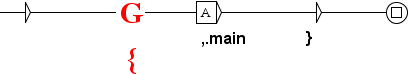
\includegraphics[width=8cm]{resources/img/graphe_restriction_A.png}
  \caption{Graphe de généralisation d'étiquetage avec une restriction sur la sous-catégorie A}
  \label{fig:graphe_restriction_A}
\end{figure}

\begin{figure}[!htb]
  \centering
  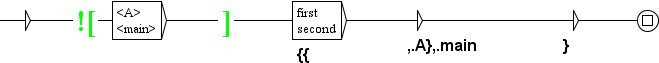
\includegraphics[width=14cm]{resources/img/graphe_restriction_A_genere.png}
  \caption{Graphe de généralisation d'étiquetage avec une restriction sur la sous-catégorie A après génération}
  \label{fig:graphe_restriction_A_genere}
\end{figure}

\begin{figure}[!htb]
  \centering
  \includegraphics[width=8cm]{resources/img/graphe_restriction_B.png}
  \caption{Graphe de généralisation d'étiquetage avec une restriction sur la sous-catégorie B}
  \label{fig:graphe_restriction_B}
\end{figure}

\begin{figure}[!htb]
  \centering
  \includegraphics[width=14cm]{resources/img/graphe_restriction_B_genere.png}
  \caption{Graphe de généralisation d'étiquetage avec une restriction sur la sous-catégorie B après génération}
  \label{fig:graphe_restriction_B_genere}
\end{figure}

\bigskip
Dans le premier cas, deux sous-étiquettes lexicales de sous-catégorie \textit{A} ont été trouvées, "premier" et "deuxième". Alors que dans le deuxième cas, une seule sous-étiquette lexicale de sous-catégorie \textit{B} a été trouvée, cette sous-étiquette lexicale contient elle-même deux autres sous-étiquettes lexicales, le contenu extrait est donc la concaténation de ce qui se trouve à l'intérieur, c'est-à-dire "deuxième troisième". Comme la sous-catégorie correspondait, la recherche n'a pas été propagée aux sous-étiquettes lexicales de niveau inférieur et la sous-étiquette lexicale "troisième" toute seule n'a pas été trouvée.

Par ailleurs, on remarque plusieurs choses; tout d'abord, le contexte droit négatif contient maintenant la catégorie du token principal et la sous-catégorie recherchée. De plus, les éléments trouvés sont doublement étiquetés, avec les deux catégories imbriquées.

\bigskip
Un graphe de généralisation d'étiquetage ne doit pas contenir un chemin sans restriction et un chemin avec restriction pour la même catégorie, à cause de l'ambiguïté générée, sauf en utilisant des poids sur les chemins (voir section~\ref{Transducers}), comme le montre la figure~\ref{fig:graphe_poids}.

\begin{figure}[!htb]
  \centering
  \includegraphics[width=10cm]{resources/img/graphe_poids.png}
  \caption{Graphe avec des poids pour éviter les ambiguïtés}
  \label{fig:graphe_poids}
\end{figure}

\bigskip
\subsubsection{Remplacement de la catégorie}

Dans certains cas, il peut arriver que l'on veuille modifier la catégorie qui sera étiquetée sur les sous-étiquettes lexicales que l'on extrait par un graphe de généralisation d'étiquetage. Par exemple dans le cas suivant :


\emph{\{de \{\{janvier,.mois\} \{2017,.année\},.date\} à \{\{novembre,.mois\} \{2018,.année\},.date\},.période\}}


\bigskip
En utilisant un graphe de généralisation d'étiquetage avec restriction pour extraire les années, les sous-étiquettes lexicales nouvellement trouvées seraient étiquetées de la façon suivante :


\emph{\{\{2017,.année\},.période\}} et \emph{\{\{2018,.année\},.période\}}

\bigskip
Ici, on voudrait remplacer "période" qui ne représente pas très bien la catégorie de ces sous-étiquettes lexicales par "date".


Pour cela il est possible de préciser la catégorie finale à obtenir, en l'ajoutant (après un point) à la sous-catégorie à rechercher.

\bigskip
Voir les figures~\ref{fig:graphe_remplacement} et~\ref{fig:graphe_remplacement_genere}.


\begin{figure}[!htb]
  \centering
  \includegraphics[width=10cm]{resources/img/graphe_remplacement.png}
  \caption{Graphe avec remplacement de la catégorie finale}
  \label{fig:graphe_remplacement}
\end{figure}

\begin{figure}[!htb]
  \centering
  \includegraphics[width=10cm]{resources/img/graphe_remplacement_genere.png}
  \caption{Graphe avec remplacement de la catégorie finale après génération}
  \label{fig:graphe_remplacement_genere}
\end{figure}

\section{Les résultats d'une cascade}

\subsection{Affichage des résultats de la cascade}
\label{subsec:resultsCascade}

Le résultat de l'application d'une cascade est un fichier d'index (\textit{concord.ind}), comme c'est le cas
lors d'une recherche de motif avec \textit{"Locate pattern"}. Ce fichier d'index contient toutes les séquences
reconnues conformément aux règles fixées dans Unitex.

\bigskip
\noindent Pour afficher une concordance, il suffit de cliquer sur le bouton "Build concordance"
(comme décrit au chapitre \ref{chap-advanced-grammars}) dans la menu "Text / Located sequences".
La figure \ref{fig13-04} présente un échantillon de concordance d'une cascade qui reconnaît les entités
nommées.


\begin{figure}[!htb]
  \centering
  \includegraphics[width=14cm]{resources/img/fig13-04.png}
  \caption{Concordance de CasSys dans Unitex}
  \label{fig13-04}
\end{figure}

\subsection{Les différents fichiers résultats d'une cascade}

CasSys conserve tous les textes créés par chaque graphe  de la cascade. Ceci peut être
utile  pour des tests, le débugage ou la vérification de différents résultats de la cascade. Il est
alors possible de corriger les erreurs selon l'ordre d'application des graphes ou de trouver des
erreurs dans leur écriture. Il est pratique d'ajouter dans la sortie d'un transducteur le nom de ce
dernier, afin de voir dans le résultat final quel motif a été reconnu par quel graphe.

Si l'on applique une cascade au texte exemple.txt, deux répertoires sont créés:
\verb+exemple_snt+ et \verb+exemple_csc+.
Les fichiers créés dans \verb+exemple_csc+ sont les résultats obtenus par
chaque graphe. Ces fichiers sont intitulés selon le numéro du graphe qui les a produit. Par exemple, si le
troisième graphe reconnaît un motif, les résultats de l'application de ce graphe seront stockés dans le 
répertoire  \verb+exemple_3+\newline\verb+_0_snt+ le fichier \verb+exemple_3_0.snt+ contiendra le texte modifié.

\subsection{Un texte au format de type XML pour les étiquettes lexicales}

En sortie, le résultat est fourni sous deux formes~: le texte résultant directement de l'application des transducteurs, et un format de type XML dans lequel les étiquettes lexicales ont été transformées en XML.
Ce changement est fait dans le but de proposer un texte plus manipulable  à l'utilisateur final.
A partir de ce format, il est possible d'utiliser l'un des nombreux outils de traitement du XML.
Il est également facile d'appliquer des transducteurs supplémentaires afin d'obtenir la sortie souhaitée.
Le texte résultant directement des transducteurs est sauvegardé dans le fichier  \verb+exemple_csc.raw+, et la version  XML-isée est dans le fichier \verb+exemple_csc.txt+.

Plus précisement, les étiquettes lexicales sont dans le format suivant~:\\
\begin{tabular}{c}
\texttt{
\{forme.lemme,code1+code2:flex1:flex2\}}
\end{tabular}\\
La sortie de type XML correspondante a le format suivant~:\\
\begin{tabular}{ll}
\texttt{<csc>}&\\
	&\texttt{<form>forme</form>}\\
	&\texttt{<lem>lemme</lem>}\\
	&\texttt{<code>code1</code>}\\
	&\texttt{<code>code2</code>}\\
	&\texttt{<inflect>flex1</inflect>}\\
	&\texttt{<inflect>flex2</inflect>}\\
\texttt{</csc>}&\\
\end{tabular}

La DTD de notre format est la suivante~:

\begin{tabular}{l}
\texttt{<?xml version="1.0" encoding="ISO-8859-1"?>}\\
\texttt{<!ELEMENT text (\#PCDATA|csc)*>}\\
\texttt{<!ELEMENT csc (form,lem?,code*,inflect*) >}\\
\texttt{<!ELEMENT form (\#PCDATA|csc)*>}\\
\texttt{<!ELEMENT lem (\#PCDATA)>}\\
\texttt{<!ELEMENT code (\#PCDATA)>}\\
\texttt{<!ELEMENT inflect (\#PCDATA)>}\\
\end{tabular}




\chapter{Utilisation des programmes externes}
\label{chap-external-programs}
Ce chapitre présente l’utilisation des différents programmes qui composent Unitex. Ces
programmes, qui se trouvent dans le répertoire \verb+Unitex/App+, sont appelés automatiquement par
l'interface (en fait, \verb+UnitexToolLogger+ est appelé, afin de réduire de manière importante la taille du fichier zip).
Il est possible de voir les commandes qui ont été exécutées en cliquant sur  "Info>Console". Il est aussi possible de voir les options des differents programmes dans "Info>Help on commands" (voir Figure \ref{fig-help}). Remarquons que tous les programmes Unitex possèdent l'option \verb$-h$/\verb$--help$.

\bigskip
\begin{figure}[!ht]
\begin{center}
\includegraphics[width=14cm]{resources/img/fig11-1.png}
\caption{Help on commands\label{fig-help}}
\end{center}
\end{figure}

\bigskip
\noindent IMPORTANT: plusieurs programmes utilisent le répertoire du texte (\verb+mon_texte_snt+).
Ce répertoire est créé par l’interface graphique après la normalisation du texte. Si vous travaillez en ligne de commande, vous devrez créer ce répertoire vous-même après l’exécution du programme
\verb+Normalize+.\index{Répertoire!texte}

\bigskip
\noindent IMPORTANT (2): lorsqu’un paramètre contient des espaces, vous devez l’entourer de
guillemets pour qu’il ne soit pas considéré comme plusieurs paramètres.

\index{Texte!répertoire}\index{Programmes externes!\verbc{Normalize}}\index{\verbc{Normalize}}

\bigskip
\noindent ATTENTION (3): beaucoup de programmes utilisent un fichier \verb+Alphabet.txt+. Cette
information peut être omise pour l'ensemble de ces programmes. Dans ce cas, une définition (par
défaut) de lettres est utilisée (voir \verb+u_is_letter+ dans le fichier source\verb$Unicode.cpp$).


\section{Création de fichiers log}\index{Création de fichiers log}
\label{section-creating-log-files}

\bigskip
\begin{figure}[!ht]
\begin{center}
\includegraphics[width=10cm]{resources/img/fig11-1a.png}
\caption{Configuration de fichiers log\label{fig-logging-config}}
\end{center}
\end{figure}

Vous pouvez créer des fichiers \verb+log+ des programmes externes exécutés.
Ces fichiers log peuvent être utiles pour le débogage ou des tests de régression. Vous avez juste
besoin d'activer cette fonctionnalité dans le cadre Préférences. Vous devez simplement choisir un
répertoire de fichiers log dans lequel tous les fichiers sont stockés, et cocher la case "Produce
log"
En cliquant sur le bouton "Clear all logs" vous supprimez tous les fichiers log éventuellement
contenus dans ce répertoire. Désormais, toute nouvelle exécution du promme produit un fichier
\verb+unitex_log_XXX.ulp+ dans le répertoire de fichiers log. \verb+XXX+ représente le numéro de
log qui se trouve dans la console (voir section suivante).



\section{La console}\index{Console}
\label{section-console}
Lorsque Unitex lance un programme externe, la ligne de commande appelée est mémorisée dans la
console. Pour la voir, cliquez sur Info ``> Console''. Quand une commande n'émet aucun message
d'erreur, elle est affichée avec une icône verte. Sinon, l'icône est un triangle rouge sur lequel
vous pouvez cliquer pour voir les messages d'erreur, comme indiqué sur la figure \ref{fig-console}
. Ceci est utile lorsque un message d'erreur se produit si vite que vous ne pouvez pas le lire. Si
une commande a été enregistrée, son numéro de log apparaît dans la deuxième colonne. Notez que vous
pouvez exporter toutes les commandes affichées dans la console vers le presse-papiers avec Ctrl + C.

\bigskip
\begin{figure}[!ht]
\begin{center}
\includegraphics[width=15cm]{resources/img/fig11-2.png}
\caption{Console\label{fig-console}}
\end{center}
\end{figure}

\section{Unitex JNI}
\index{Unitex JNI}
\label{section-unitex-JNI}

Vous pouvez utilisez Unitex avec JNI by en incluant les imports suivants : 
\begin{verbatim}
import fr.umlv.unitex.jni.UnitexJni;
import java.io.*;
import fr.umlv.unitex.*;
\end{verbatim}
Ceci vous permet de charger en mémoire les dictionnaires (.bin), les grammaires ou graphes dictionnaires (.fst2) et les fichiers alphabet et de les garder en mémoire de manière persistante. Vous utilisez alors le nom de fichier renvoyé par la foncton loadPersistent*.

\begin{verbatim}
String persistentAlphabet = UnitexJni.loadPersistentAlphabet("/.../unitex/French/Alphabet.txt");
String persistentFst2 = UnitexJni.loadPersistentFst2("/.../unitex/French/Dela/fogg-r.fst2");
String persistentDictionary = UnitexJni.loadPersistentDictionary(
		"/.../unitex/French/Dela/communesFR+.bin");
\end{verbatim}


\section{Paramètres de codage des fichiers textes}\index{Paramètres de codage des fichiers textes}\index{Fichier!texte!paramètres de codage}
\label{section-text-file-encoding-parameters}
Unitex utilise Unicode pour les fichiers textes \ref{unicode-encoding}. Tous les programmes qui
lisent ou écrivent des fichiers textes partagent les mêmes paramètres d'encodage. Les formats
possibles sont utf16le-bom, utf16le-no-bom, utf16be-bom, utf16be-no-bom, utf8-bom, utf8-no-bom, qui
correspondent à Unicode Big-Endian, Little-Endian et UTF-8, avec ou sans "Unicode byte order mark"
(bom) au début du fichier. Pour le format d'entrée, vous pouvez spécifier plusieurs encodages *-bom
(avec bom) codage séparées par des virgules, mais seulement un encodage *-no-bom (sans bom).

\bigskip
\noindent \textbf{OPTIONS:}
\begin{itemize}
\item \verb+-k=ENCODING+/\verb+--input_encoding=ENCODING+: format du texte source. Peut contenir
plusieurs valeurs séparées par des virgules;
\item \verb+-q=ENCODING+/\verb+--output_encoding=ENCODING+: format du texte de sortie. 
\end{itemize}

\noindent Par défaut, les valeurs sont: \verb+--input_encoding=utf16le-bom,utf16be-bom,utf8-bom+
\newline \verb+--output_encoding=utf16le-bom+.


\section{BuildKrMwuDic}\index{Programmes externes!\verbc{BuildKrMwuDic}}\index{\verbc{BuildKrMwuDic}}
\index{Génération du dictionnaire des mots composés coréens}\index{Dictionnaire!mots composés
coréens}
\verb+BuildKrMwuDic [OPTIONS] dic+

\bigskip
\noindent Ce programme génère des graphes de flexion pour les mots composés à partir d'un tableau
\verb+dic+ qui décrit chaque constituant de chaque mot composé
\bigskip
\noindent \textbf{OPTIONS:}
\begin{itemize}
\item \verb+-o GRF+/\verb+--output=GRF+: fichier \verb+.grf+ à produire;
\item \verb+-d DIR+/\verb+--directory=DIR+: répertoire de flexion qui contient les graphes de
	flexion nécéssaires pour produire les variantes morphologiques des racines;
\item \verb+-a ALPH+/\verb+--alphabet=ALPH+: fichier alphabet à utiliser;
\item \verb+-b BIN+/\verb+--binary=BIN+:  dictionnaire des mots simples de type \verb+.bin+ à
	utiliser;
\end{itemize}






\section{CasSys}\index{Programmes externes!\verbc{CasSys}}\index{\verbc{CasSys}}
\index{Cascade de transducteurs}
\verb+Cassys [OPTIONS] <snt>+

\bigskip
\noindent Ce programme applique une liste ordonnée de grammaires à un texte et construit un index
des occurrences trouvées.
\bigskip
\noindent \textbf{OPTIONS:}
\begin{itemize}
\item \verb+-a ALPH+/\verb+--alphabet=ALPH+: fichier alphabet de la langue;
\item \verb+-r X+/\verb+--transducer_dir=X+: prend un transducteur dans le répertoire \verb+X+ (cela évite de 
		donner le chemin complet pour chaque transducteur; remarquons que \verb+X+ doit se
		terminer par un antislash;
	\item \verb+-w DIC/--morpho=DIC+: indique que \verb+DIC+ est un \verb+.bin+ dictionnaire à utiliser en mode morphologique.
		Utiliser autant de  \verb+-m XXX+ qu'il y a de \verb+.bin+. Il est également possible de séparer plusieurs \verb+.bin+ par le caractère deux-points.

\item \verb+-l TRANSDUCERS_LIST+/\verb+--transducers_list=TRANSDUCERS_LIST+: fichier
		contenant la liste des transducteurs avec leur mode d'application;
\item \verb+-s transducer.fst2+/\verb+--transducer_file=transducer.fst2+: un transducteur à
		appliquer;
\item \verb+-m output_policy+/\verb+--transducer_policy=output_policy+: le mode
		d'application du transducteur spécifié;
\item \verb+-t TXT+/\verb+--text=TXT+: le fichier texte avec l'extension \verb+.snt+ à modifier;
\item \verb+-i+/\verb+--in_place+: signifie qu'il faut utiliser les mêmes répertoires \verb+csc/snt+
	pour chaque transducteur;
\item \verb+-d+/\verb+--no_create_directory+: signifie que tous les répertoires \verb+snt/csc+
	existent déjà et n'ont pas besoin d'être crées;
\item \verb+-g minus+/\verb+--negation_operator=minus+: utilise \verb+moins+ comme opérateur de
	négation pour les graphes version Unitex 2.0;
\item \verb+-g tilde+/\verb+--negation_operator=tilde+: utilise \verb+tilde+ comme opérateur de
	négation (par défaut);
\item \verb+--standoff=+: indique le chemin et le nom du fichier indiquant le modèle de standoff et lance la création du standOff du texte;
\item \verb+-h+/\verb+--help+: affiche cette aide
\end{itemize} 	


\bigskip
\noindent CasSys applique une liste de grammaires à un texte et sauve les séquences reconnues dans
un fichier index nommé \verb+concord.ind+ stocké dans le répertoire texte.
Le fichier cible doit être un fichier snt avec son répertoire \verb+_snt+. 
Le fichier contenant la liste des transducteurs est un fichier dans lequel chaque ligne contient le
nom complet du transducteur suivi de son mode d'application.

\bigskip
\noindent A la place d'une liste, vous pouvez spécifier chaque fichier et mode d'application par un
ensemble de couple d'arguments pour représenter la liste \verb+-s/--transducer\_file+ et
\verb+-m/--transducer\_policy+ 
      
\bigskip
\noindent Le mode d'application peut être MERGE ou REPLACE.
      
\bigskip
\noindent L'option de fichier, l'option alphabet et l'option fichier liste de transducteurs sont
obligatoires
     
\bigskip
\noindent Comme le programme Locate, ce programme enregistre les références des occurrences dans un
fichier \verb+concord.ind+ stocké dans le répertoire \verb+_snt+ du texte.
Le fichier \verb+concord.ind+ produit est dans le même format que celui décrit chapitre
\ref{chap-file-formats} , mais la cascade peut être formée de graphes appliqués en mode merge ou
replace, de ce fait \#M ou \#R à la première ligne du fichier \verb+concord.ind+ n'a pas de sens dans ce contexte.



\section{CheckDic}\index{Programmes externes!\verbc{CheckDic}}\index{\verbc{CheckDic}}
\index{Vérification du format d'un dictionnaire}\index{Dictionnaire!vérification}
\verb+CheckDic [OPTIONS] dic+

\bigskip
\noindent Ce programme effectue la vérification du format d’un dictionnaire de type DELAS ou
DELAF.\verb+dic+ qui correspond au nom du dictionnaire à vérifier

\bigskip
\noindent \textbf{OPTIONS:}
\begin{itemize}
\item \verb+-f+/\verb+--delaf+: vérifie un dictionnaire de formes fléchies;
\item \verb+-s+/\verb+--delas+: vérifie un dictionnaire de formes canoniques;
\item \verb+-r+/\verb+--strict+: vérification stricte de la syntaxe, la déspécialisation des points
	et virgules;
\item \verb+-t+/\verb+--tolerate+: tolère des points et des virgules non déspécialisés (par défaut);
\item \verb+-n+/\verb+--no_space_warning+: tolère des espaces dans les codes
	grammaticaux/sémantiques/flexionnels;
\item \verb+-p+/\verb+--skip_path+: n'affiche pas le chemin complet du dictionnaire (utiles pour la
		compatibilité de fichiers de log sur plusieurs systèmes);
\item \verb+-a ALPH+/\verb+--alphabet=ALPH+: indique le fichier alphabet à utiliser. 
\end{itemize}

\bigskip
\noindent Le programme teste la syntaxe des lignes du dictionnaire. Il dresse également la liste des
caractères présents dans les formes fléchies et canoniques, la liste des codes grammaticaux
et syntaxiques ainsi que la liste des codes flexionnels utilisés. Les résultats de la vérification
sont stockés dans un fichier nommé \verb+CHECK_DIC.TXT+.\index{Fichier!\verbc{CHECK_DIC.TXT}}

\bigskip
\noindent Le choix de \verb+--strict+ permet de détecter l'utilisation de points non déspécialisés
dans la forme fléchie ou de virgules non déspécialisées dans la forme canonique. L'option
\verb+--tolerate+ se comporte comme dans les versions Unitex 2.0 et antérieures et ne les détecte
pas.





\section{Compress}\index{Programmes externes!\verbc{Compress}}\index{\verbc{Compress}}
\index{Compression des dictionnaires}
\label{section-compress}
\verb+Compress [OPTIONS] dictionary+
\index{Dictionnaire!DELAF}\index{Dictionnaire!compression}
\index{Fichier!\verbc{.dic}}\index{Fichier!\verbc{.bin}}\index{Fichier!\verbc{.inf}}

\bigskip
\noindent \textbf{OPTIONS:}
\begin{itemize}
\item \verb+-o BIN+/\verb+--output=BIN+: définit le fichier de sortie. Par défaut, un fichier
	\verb+xxx.dic+ produit un fichier \verb+xxx.bin+;
\item \verb+-f+/\verb+--flip+: indique que les formes fléchies et canoniques doivent être inversées
dans le dictionnaire comprimé. Cette option est utilisée pour construire un dictionnaire inversé
nécessaire au programme \verb+Reconstrucao+;
\item \verb+-s+/\verb+--semitic+: indique que l'algorithme de compression pour langue sémitique doit
être utilisé. Cette option utilisée avec des langues sémitiques comme l'arabe réduit sensiblement la
taille du dictionnaire produit;
\item \verb+--v1+: produit un fichier \verb+.bin+ ancienne manière;
\item \verb+--v2+: produit un fichier \verb+.bin+ nouvelle manière, mieux comprimé et sans
	limitation de taille de fichier à 16 Mb (par défaut)
\end{itemize}

\bigskip
\noindent Ce programme prend en paramètre un dictionnaire DELAF et le compresse.

La compression d’un dictionnaire \verb+dico.dic+ produit deux fichiers:
\begin{itemize}
  \item \verb+dico.bin+: fichier binaire contenant l’automate minimal des formes fléchies du
  	  dictionnaire ;
  \item \verb+dico.inf+: fichier texte contenant des formes comprimées permettant de reconstruire
les lignes du dictionnaire à partir des formes fléchies contenues dans l’automate.
\end{itemize}

\bigskip
\noindent Pour plus de détails sur les formats de ces fichiers, voir chapitre
\ref{chap-file-formats}.






\section{Concord}\index{Programmes externes!\verbc{Concord}}\index{\verbc{Concord}}\index{Concordance}
\label{section-Concord}
\index{Texte!modification}\index{Modification du texte}
\verb+Concord [OPTIONS] <index>+

\bigskip
\noindent Ce programme prend en paramètre un fichier d’index de concordance produit par le
programme \verb+Locate+ et produit une concordance. Il peut également produire une version
du texte modifiée prenant en compte les transductions associées aux occurrences. Voici la
description des paramètres:


\bigskip
\noindent \textbf{OPTIONS:}
\begin{itemize}
  \item \verb+-f FONT+/\verb+--font=FONT+: nom de la police de caractères à utiliser si la
  	  sortie est fichier HTML;
  \item \verb+-s N+/\verb+--fontsize=N+: taille de la police si la sortie est fichier HTML.
  	Les paramètres concernant la police sont ignorés si la sortie n’est pas au format HTML;
  \item \verb+--only_ambiguous+: Affiche seulement les occurrences identiques avec une sortie
  	  ambiguë, dans l'odre du texte.
  \item \verb+--only_matches+: cette option définit un mode sans contexte.
	En outre si elle est utilisée avec \verb+-t/--text+, Concord n'entoure pas les séquences
	reconnues de tabulations
  \item \verb+-l X+/\verb+--left=X+: nombre de caractères à gauche des occurrences (par défaut=0).
  	  Dans le mode Thai, ceci correspond au nombre de caractères non
  	  diacritiques.\index{Contexte!concordance}
  \item \verb+-r X+/\verb+--right=X+: nombre de caractères (non diacritiques dans le mode Thai)
	à droite des occurrences (par défaut=0). Si l'occurrence est plus petite que cette valeur,
	la ligne de concordance est complétée jusqu'à \verb+right+. Si l'occurrence est plus longue
	que la valeur définie par \verb+right+, elle est néanmoins entièrement conservée.
  
  \bigskip
  NOTE: Pour \verb+--left+ et \verb+--right+, vous pouvez ajouter le caractère \verb+s+
  pour arrêter au premier symbole de fin de phrase \verb+{S}+. Par exemple, si vous mettez 
  \verb+40s+ comme valeur de gauche, le contexte gauche sera au plus à 40 caractères, moins si le \verb+{S}+ est trouvé avant.
\end{itemize}

\bigskip
\noindent \textbf{Options de tri:}\index{Tri!de concordance}
\begin{itemize}
  \item \verb+--TO+: ordre dans lequel les occurrences apparaissent dans le texte (par défaut);
  \item \verb+--LC+: contexte gauche comme premier tri, occurrence comme second tri;
  \item \verb+--LR+: contexte gauche, contexte droit;
  \item \verb+--CL+: occurrence, contexte gauche;
  \item \verb+--CR+: occurrence, contexte droit;
  \item \verb+--RL+: contexte droit, contexte gauche;
  \item \verb+--RC+: contexte droit, occurrence.
\end{itemize}
\noindent Pour plus de détails sur ces modes de tri, voir la section
\ref{section-display-occurrences}.

\bigskip
\noindent \textbf{Options de sortie:}
\begin{itemize}
  \item \verb+-H+/\verb+--html+: produit une concordance au format HTML codée en UTF-8;
  	  \index{UTF-8} (par défaut);
  \item \verb+-t+/\verb+--text+: produit une concordance au format texte Unicode; 
  \item \verb+-g SCRIPT+/\verb+--glossanet=SCRIPT+: produit une concordance pour GlossaNet
  	  au format HTML. Le fichier HTML produit est codé en UTF-8;\index{GlossaNet}
  \item \verb+-p SCRIPT+/\verb+--script=SCRIPT+: produit une concordance au format HTML où les
  	  occurrences sont liens décrits par \verb+SCRIPT+. Par exemple, si vous utilisez
  	  
  \verb$-phttp://www.google.com/search?q=$, vous obtiendrez 
  une concordance au format HTML où les occurrences sont des liens vers des requêtes Google;

\item \verb+-i+/\verb+--index+: produit un index de la concordance, qui comporte
	les occurrences (avec les sorties des grammaires, s'il y en a), précédées par
	les positions des occurrences, dans le fichier texte, exprimées en caractères;
\item \verb+-u+ \verb+offsets+/\verb+--uima=offsets+: produit un index de la concordance relatif
	fichier texte original, avant toute opération effectuée par Unitex. Offsets 
	est le fichier produit par Tokenize avec l'option \verb+--output_offsets+
%  the same as \verb+--index+, but the ending position of each occurrence is also given;
\item \verb+-e+/\verb+--xml+: produit un index xml de la concordance;
\item \verb+-w+/\verb+--xml-with-header+: produit un index xml de la concordance avec une en-tête
	xml complète;
\item \verb+--lemmatize+: produit un fichier de concordance HTML spécial utilisé par l'interface de lemmatisation
	de l'interface graphique d'Unitex.


	REMARQUE:  les options -e et -w acceptent toutes deux un fichier d'offset, comme l'accepte -u 
\item \verb+--PRLG=X,Y+: produit une concordance pour des corpus PRLG où chaque ligne
	est préfixée par l'information extraite avec l'option \verb+--PRLG+ de Unxmlize. X est le
	fichier produit par l'option \verb+--PRLG+ de Unxmlize et Y est le fichier produit par
	l'option \verb+--output_offsets+ de Tokenize. Remarquons que si cette option est utilisée en
	plus avec \verb+-u+, l'argument Y remplace l'argument de \verb+-u+;
	
\item \verb+-A+/\verb+--axis+: presque pareil que \verb+--index+, mais les nombres
	représentent le caractère médian de chaque occurrence. Pour plus d'information,
	consultez \cite{axis};
\item \verb+-x+/\verb+--xalign+: un autre fichier index, utilisé par le module d'alignement de
	texte.
	Chaque ligne est formée de 3 entiers $X$ $Y$ $Z$ suivi du contenu de l'occurrence.
	$X$ est numéro de la phrase, partant de 1. $Y$ et $Z$ sont les positions de début et de fin
	de l'occurrence dans la phrase exprimée en caractères;
\item \verb+-m TXT+/\verb+--merge=TXT+: indique au programme qu'il doit produire une version
	modifiée du texte et l'enregistrer dans le fichier dénommé
	\verb+TXT+ (voir section \ref{section-modifying-text}).
	
\item  \verb+T--export_csv+: produit un fichier avec le séparateur tabulation export.csv dans l'ordre du texte avec le 
	format suivant:
	\subitem A B C D E F, où:
	\subitem  A=nombre de lignes dans le fichier .csv
	\subitem  B=nombre de phrases
	\subitem  C= référence PRLG, si elle existe
	\subitem  D=la forme fléchie présente dans le texte
	\subitem  E=le lemme, s'il existe
	\subitem  F=les codes, s'il y en a\\
	Pour fonctionner, cette option doit re appelée pour des fichier concord.ind, qui ne contiennent pas de token
	{S} ni espace
\end{itemize}

\bigskip
\noindent \textbf{Autres options:}
\begin{itemize}
\item \verb+-d DIR+/\verb+--directory=DIR+: indique au programme qu'il ne doit pas travailler avec
	le même répertoire que \verb+<index>+ mais avec \verb+DIR+;
  \item \verb+-a ALPH+/\verb+--alphabet=ALPH+: fichier alphabet utilisé pour le tri;
  \item \verb+-T+/\verb+--thai+: option à utiliser pour les concordances en Thai.
  \index{Alphabet}\index{Fichier!alphabet}
\end{itemize}

\index{Fichier!\verbc{.html}}\index{Fichier!\verbc{.txt}}
\bigskip
\noindent Le résultat de l’application de ce programme est un fichier \verb+concord.txt+
si la concordance a été construite en mode texte, un fichier \verb+concord.html+ pour les modes
 \verb+--html+, \verb+--glossanet+ ou \verb$--script$, et un fichier texte dont le nom a été
défini par l’utilisateur si le programme a construit une version modifiée du texte.


\bigskip
\noindent En mode \verb+--html+, l’occurrence est codée comme un lien. La référence associée à ce
lien est de la forme \verb+<a href="X Y Z">+. \verb+X+ et \verb+Y+ représentent les positions de
début et de fin de l’occurrence en caractères dans le fichier \verb+text_name.snt+. \verb+Z+
représente le numéro de la phrase dans laquelle apparaît l’occurrence.







\section{ConcorDiff}\index{Programmes externes!\verbc{ConcorDiff}}\index{\verbc{ConcorDiff}}
\verb+ConcorDiff [OPTIONS] <concor1> <concor2>+

\bigskip
\noindent Ce programme prend deux fichiers de concordance et produit une page HTML montrant les
différences entre ces deux concordances (voir section
\ref{section-comparing-concordances}, page \pageref{section-comparing-concordances}). 
\verb+<concor1>+ et \verb+<concor2>+ fichiers de concordances (.ind) doivent avoir des noms  
absolus, car Unitex en déduit le texte sur lequel elles ont été calculées;

\bigskip
\noindent \textbf{OPTIONS:}
\begin{itemize}
  \item \verb+-o X+/\verb+--out=X+: page HTML de sortie;
  \item \verb+-f FONT+/\verb+--font=FONT+: police à utiliser dans le page HTML de sortie;
  \item \verb+-s N+/\verb+--size=N+: taille de police à utiliser dans le page HTML de sortie;
  \item \verb+-d/--diff_only+: ne pas afficher les séquences identiques;
\end{itemize}







\section{Convert}\index{Programmes externes!\verbc{Convert}}\index{\verbc{Convert}}
\verb+Convert [OPTIONS] <text_1> [<text_2> <text_3> ...]+

\index{Unicode}
\bigskip
\noindent Ce programme permet de transcoder des fichiers textes.

\bigskip
\noindent \textbf{OPTIONS:}
\begin{itemize}
\item \verb+-s X+/\verb+--src=X+: encodage d'entrée;
\item \verb+-d X+/\verb+--dest=X+: encodage de sortie
	(par défaut=\verb$LITTLE-ENDIAN$);
\end{itemize}

\bigskip
\noindent \textbf{Options de translitération (seulement pour l'arabe):}
\begin{itemize}
\item \verb+-F+/\verb+--delaf+: l'entrée est un DELAF et l'on veut seulement translitérer les formes
	fléchies et canoniques;
\item \verb+-S+/\verb+--delas+: l'entrée est un DELAS et l'on veut seulement translitérer les formes
	canoniques.
\end{itemize}


\bigskip
\noindent \textbf{Options de sortie:}
\begin{itemize}
\item \verb+-r+/\verb+--replace+: la conversion écrase les fichiers source (par défaut);
\item \verb+-o file+/\verb+--output=file+: nom du fichier de destination (seulement un fichier à convertir);
\item \verb+--ps=PFX+: les fichiers sources sont renommés avec le préfixe \verb+PFX+;
        (\verb+toto.txt+ $\Rightarrow$ \verb+PFXtoto.txt+);
\item \verb+--pd=PFX+: les fichiers destinations sont renommés avec le préfixe \verb+PFX+;
\item \verb+--ss=SFX+: les fichiers sources sont renommés avec le suffixe \verb+SFX+;
        (\verb+toto.txt+ $\Rightarrow$ \verb+totoSFX.txt+);
\item \verb+--sd=SFX+: les fichiers destinations sont renommés avec le suffixe \verb+SFX+.
\end{itemize}

\bigskip
\noindent \textbf{Options HTML:}

\noindent \verb+Convert+ offre des options spéciales pour les fichiers HTML. Vous pouvez utiliser  une combinaison des options suivantes:

\begin{itemize}
\item \verb+--dnc+ (Decode Normal Chars): des séquences comme \verb+&eacute;+
	\verb+&#120;+ et \verb+&#xF8;+ sont décodées comme un unique caractère
	unicode, sauf si elles representent un caractère de contrôle HTML;
  
  \item \verb+--dcc+ (Decode Control Chars): \verb+&lt;+ \verb+&gt;+
  	  \verb+&amp;+ et \verb+&quot;+ sont décodés comme \verb+<+ \verb+>+
  \verb+&+ et les quote (de même pour leur représentation  décimales et hexadécimales);
  
  \item \verb+--eac+ (Encode All Chars): chaque caractère non supporté par l'encodage de sortie
  	  est représenté par une chaîne comme \verb+&#457;+
  
  \item \verb+--ecc+ (Encode Control Chars): \verb+<+ \verb+>+
  	  \verb+&+ et les  quote sont encodés par \verb+&lt;+ \verb+&gt;+
  	  \verb+&amp;+ et \verb+&quot;+
\end{itemize} 

\noindent Par défaut, toutes les options HTML sont désactivées.

\bigskip
\noindent \textbf{Autres options:}
\begin{itemize}
\item \verb+-m+/\verb+--main-names+: imprime la liste des noms principaux des encodage;
\item \verb+-a+/\verb+--aliases+: imprime la liste des alias d'encodage;
\item \verb+-A+/\verb+--all-infos+: imprime toutes les information concernant tous les encodages;
\item \verb+-i X+/\verb+--info=X+: imprime toutes les information concernant l'encodage X.
\end{itemize}

\bigskip
\noindent Les encodages prennent leurs valeurs dans la liste suivante  (liste non exhaustive, voir
	ci-dessous):

\bigskip
\verb$FRENCH$

\verb$ENGLISH$

\verb$GREEK$

\verb$THAI$

\verb$CZECH$

\verb$GERMAN$

\verb$SPANISH$

\verb$PORTUGUESE$

\verb$ITALIAN$

\verb$NORWEGIAN$

\verb$LATIN$ (default latin code page)

\verb$windows-1252$: Microsoft Windows 1252 - Latin I (Western Europe \& USA)

\verb$windows-1250$: Microsoft Windows 1250 - Central Europe

\verb$windows-1257$: Microsoft Windows 1257 - Baltic

\verb$windows-1251$: Microsoft Windows 1251 - Cyrillic

\verb$windows-1254$: Microsoft Windows 1254 - Turkish

\verb$windows-1258$: Microsoft Windows 1258 - Viet Nam

\verb$iso-8859-1  $: ISO 8859-1  - Latin 1 (Europe de l'ouest \& USA)

\verb$iso-8859-15 $: ISO 8859-15 - Latin 9 (Western Europe \& USA)

\verb$iso-8859-2  $: ISO 8859-2  - Latin 2 (Eastern and Central Europe)

\verb$iso-8859-3  $: ISO 8859-3  - Latin 3 (Southern Europe)

\verb$iso-8859-4  $: ISO 8859-4  - Latin 4 (Northern Europe)

\verb$iso-8859-5  $: ISO 8859-5  - Cyrillic

\verb$iso-8859-7  $: ISO 8859-7  - Greek

\verb$iso-8859-9  $: ISO 8859-9  - Latin 5 (Turkish)

\verb$iso-8859-10 $: ISO 8859-10 - Latin 6 (Nordic)

\verb$next-step   $: NextStep code page

\verb$LITTLE-ENDIAN$

\verb$BIG-ENDIAN$

\verb$UTF8$







\section{Dico}\index{Programmes externes!\verbc{Dico}}\index{\verbc{Dico}}
\index{Dictionnaire!application}
\verb+Dico [OPTIONS] <dic_1> [<dic_2> <dic_3>...]+

\bigskip
\noindent Ce programme applique des dictionnaires à un texte. Le texte doit avoir été découpé en
unités lexicales par le programme \verb+Tokenize+.

\bigskip
\noindent \textbf{OPTIONS:}
\begin{itemize}
\item \verb+-t TXT+/\verb+--text=TXT+: nom complet du fichier texte \verb+.snt+;
\item \verb+-a ALPH+/\verb+--alphabet=ALPH+: le fichier alphabet à utiliser;
\item \verb+-m DICS+/\verb+--morpho=DICS+: ce paramètre optionnel liste
	les dictionnaires du mode morphologique, si la présence de dictionnaires
	\verb+.fst2+ rend cette information nécessaire. \verb+DICS+ représente une liste de fichiers \verb+.bin+ (avec leur nom
		complet) séparés par des points-virgules;
\item \verb+-K+/\verb+--korean+: indique à \verb$Dico$ qu'il travaille sur du coréen;
\item \verb+-s+/\verb+--semitic+: indique à \verb$Dico$ qu'il travaille sur une langue sémitique
	(nécessaire  si \verb$Dico$ doit compresser un dictionnaire);
\item \verb+-u X+/\verb+--arabic_rules=X+: désigne le fichier de configuration des règles
	typographiques de l'arabe;.
\item \verb+r X+/\verb+--raw=X+: indique que \verb$Dico$ devrait simplement produire un fichier de
	sortie X contenant les mots simples et composés, sans exiger un répertoire texte. Si X est
	omis, les résultats sont affichés sur la sortie standard.
\end{itemize}

\bigskip
\noindent \verb+<dic_i>+ représente le chemin d’accès complet à un dictionnaire. Le dictionnaire
doit être soit un dictionnaire compressé au format \verb+.bin+ (obtenu avec le programme
	\verb+Compress+) soit un graphe dictionnaire au format\verb+.fst2+ (voir section
\ref{section-applying-dictionaries}, page \pageref{section-applying-dictionaries}).
	\index{Fichier!\verbc{.bin}} Il est possible de donner des priorités aux dictionnaires. Pour
	les détails voir section \ref{section-dictionary-priorities}.

\bigskip
\noindent Le programme \verb+Dico+ produit les fichiers suivants et les sauve dans le répertoire du
texte

\begin{itemize}
  \index{Fichier!\verbc{dlf}}\index{Fichier!\verbc{dlc}}\index{Fichier!\verbc{err}}\index{Fichier!\verbc{stat_dic.n}}
  \item \verb+dlf+: dictionnaire des mots simples du texte;
  \item \verb+dlc+: dictionnaire des mots composés du texte;
  \item \verb+err+: liste des mots inconnus du texte;
  \item \verb+tags_err+: mots simples inconnus qui ne sont pas reconnus par le fichier
  	  \verb+tags.ind+;
  \item \verb+tags.ind+ : séquences à insérer dans l'automate du texte
  (see section \ref{section-dictionary-graphs}, page \pageref{section-dictionary-graphs});
  \item \verb+stat_dic.n+: fichier contenant les nombres de mots simples, composés et inconnus du
  	  texte.
\end{itemize}

\bigskip
\noindent NOTE: Les fichiers\verb+dlf+, \verb+dlc+, \verb+err+ and \verb+tags_err+ ne sont pas triés. Utilisez le programme \verb+SortTxt+ pour le faire.



\section{DumpOffsets}\index{Programmes externes!\verbc{DumpOffsets}}\index{\verbc{DumpOffsets}}
\label{section-DumpOffsets}
\textbf{Utilisation:} \verb+DumpOffsets [OPTIONS] <txt>+

\bigskip
\noindent\verb+<txt>: fichier d'offsets d'origine+

\bigskip
\noindent Ce programme permet d'étudier et d'utiliser les fichiers de correspondance d'Offsets, manipulé par
certains outils Unitex comme Unxmlize, Normalize, Fst2Txt, Tokenize, Concord et GrfTest.


\bigskip
\noindent \textbf{OPTIONS:}

\begin{itemize} 	 
  \item \verb+-o X+/\verb+--old=X+: nom du fichier d'origine 
  \item \verb+-n X+/\verb+--new=X+:  nom du fichier d'arrivée
  \item \verb+-p X+/\verb+--output=X+: nom du fichier de sortie
  \item \verb+-f+/\verb+--full+: ajouter le texte courant
  \item \verb+-q+/\verb+--quiet+: ne pas afficher de message
  \item \verb+-c+/\verb+--no_escape_sequence+: don't escape text sequence 	 
  \item \verb+-h+/\verb+--help+: cet aide 	 
\end{itemize}

\noindent Exemple: 
\begin{verbatim}
	 UnitexToolLogger Normalize -r .\resource\Norm.txt .\work\text_file.txt 	 
	         --output_offsets .\work\text_file_offset.txt 	 
	 UnitexToolLogger DumpOffsets -o .\work\text_file_offset.txt -n .\work\text_file_offset.snt 	 
	        -p .\work\dump\dump_offsets.txt .\work\text_file_offset.txt 	 
\end{verbatim}

\bigskip
\noindent \textbf{Autre Utilisation:} \verb+DumpOffsets [-m/--merge] [OPTIONS] <txt>+

\bigskip
\noindent \verb+<txt>: fichier d'offsets d'origine+

\bigskip
\noindent Fusionner deux fichiers d'offsets produits par deux modifications successives du texte.

\bigskip
\noindent \textbf{OPTIONS:}

\begin{itemize} 	 
  \item \verb+-o X+/\verb+--old=X+: nom du fichier d'origine
  \item \verb+-n X+/\verb+--output=X+: nom du fichier d'offset issu de la fusion
\end{itemize}

\bigskip
\noindent \textbf{Autre Utilisation:} \verb+DumpOffsets [-v/--convert_modified_to_common] [OPTIONS] <txt>+

\bigskip
\noindent \verb+<txt>: fichier d'offsets d'origine+

\bigskip
\noindent Crée un fichier d'offset des chaines identiques dans le fichier original et le fichier modifié.
Au moins une taille doit être fournie.	 

\bigskip
\noindent \textbf{OPTIONS:}
	  	 
\begin{itemize} 	 
  \item \verb+-s N+/\verb+--old_size=N+: taille en caractère de la version d'origine du fichier texte
  \item \verb+-S N+/\verb+--new_size=N+: taille en caractère de la version d'arrivée du fichier texte
  \item \verb+-p X+/\verb+--output=X+: nom du fichier d'offsets courant	 
  \item \verb+-h+/\verb+--help+: cet aide
\end{itemize} 	 

\bigskip
\noindent \textbf{Autre Utilisation:} \verb+DumpOffsets [-M/--convert_modified_to_common] [OPTIONS] <txt>+

\bigskip
\noindent \verb+<txt>: fichier d'offsets d'origine+

\bigskip
\noindent Crée un fichier d'offsets à partir des offsets des chaines identiques dans le fichier original et le fichier modifié.
Il faut obligatoirement spécifier les deux tailles.
	
\bigskip
\noindent \textbf{OPTIONS:}
	  	 
\begin{itemize} 	 
  \item \verb+-s N+/\verb+--old_size=N+: taille en caractère de la version d'origine du fichier texte
  \item \verb+-S N+/\verb+--new_size=N+: taille en caractère de la version d'arrivée du fichier texte
  \item \verb+-p X+/\verb+--output=X+: nom du fichier d'offsets courant	 
  \item \verb+-h+/\verb+--help+: cet aide	 
\end{itemize} 	 

\bigskip
\noindent \textbf{Autre Utilisation:} \verb+DumpOffsets -o <list_of_position_file_to_read.txt>+

\bigskip
\noindent \verb+<list_of_position_file_to_read.txt>+ est un fichier avec seulement un nombre par ligne (une position).

\bigskip
\noindent Ceci convertit une liste de positions en utilisant le fichier d'offsets.
	  Le fichier créé contient à chaque ligne la nouvelle position suivi d'un +  si le caractère à cette position 
	  est dans le fichier d'arrivée, suivi d'un - si le caractère a été supprimé.
	  	 
\begin{itemize}
  \item \verb+-p <list_to_create> -T <offset_file_to_read>+
\end{itemize} 	 

\noindent Utiliser \verb+-t+ à la place de \verb+-T+ produit la traduction inverse.	 






\section{DumpOffsets}\index{Programmes externes!\verbc{DumpOffsets}}\index{\verbc{DumpOffsets}}
\label{section-DumpOffsets}

\noindent Ce programme permet d'étudier et d'utiliser les fichiers de correspondance d'Offsets, manipulé par
certains outils Unitex comme Unxmlize, Normalize, Fst2Txt, Tokenize, Concord et GrfTest.

\bigskip
\begin{verbatim}
DumpOffsets --merge -o <fichier_offsets1> <fichier_offsets2>
  -p <fichier_offset12>
\end{verbatim}
En entrée, le fichier offsets1 (\ref{subsection-offsets-diff}, page \pageref{subsection-offsets-diff})) contient la correspondant des offsets entre un fichier en version A
et un fichier en version B, et offset2 contient la correspondant des offsets entre ce fichier en version B
et en version C, le fichier fichier\_offset12 résultant aura la correspondance entre les versions A et B.

\begin{verbatim}
DumpOffsets [OPTIONS] -o <fichier_version1> -n <fichier_Version2>
  <fichier_offset> -p <fichier_dump>
\end{verbatim}
\bigskip

\noindent \textbf{OPTIONS:}
\begin{itemize}
\item \verb+-f/--full+: Inclus des informations plus complètes
\end{itemize}

En entrée, le fichier fichier\_offset contient la correspondant des offsets entre le fichier\_version1 et le
fichier\_version2. En sortie, le fichier texte <fichier\_dump> contiendra la comparaison des séquences entre les
2 fichiers et vérifiera leur cohérence. Ce fichier est destinée à une lecture manuelle, afin d'étudier le contenu
du fichier d'offset


\bigskip
\begin{verbatim}
DumpOffsets [OPTIONS] --convert_modified_to_common 
  <fichier_offset_différence> -p <fichier_offset_zone_commune>
\end{verbatim}
\bigskip

\noindent \textbf{OPTIONS:}
\begin{itemize}
\item \verb+-s N/--old_size=N+: Contient la taille en caractère de la version d'origine du fichiet texte
\item \verb+-S N/--new_size=N+: Contient la taille en caractère de la version d'arrivée du fichiet texte
\end{itemize}
Il faut obligatoirement spécifier une des deux tailles. Pour un fichier encodé en UTF16BE\_BOM, c’est la taille en
octets, auquel on retranche 2 pour les 2 octets de signature BOM et que l’on divise ensuite par 2 car chaque
caractère unicode prend 2 octets. En UTF8, la correspondance n’est pas immédiate.

Converti un fichier d'offset indiquant les caractères supprimés (tel que fournis par les autres outils Unitex) en fichier
indiquant les plages de caractères identiques (\ref{subsection-offsets-common}).

\bigskip
\begin{verbatim}
DumpOffsets [OPTIONS] --convert_common_to_modified
  <fichier_offset_zone_commune> -p <fichier_offset_différence>
\end{verbatim}
\bigskip

\noindent \textbf{OPTIONS:}
\begin{itemize}
\item \verb+-s N/--old\_size=N+: Contient la taille en caractère de la version d'origine du fichier texte
\item \verb+-S N/--new\_size=N+: Contient la taille en caractère de la version d'arrivée du fichier texte
\end{itemize}
Il faut obligatoirement spécifier les deux tailles.

Converti un fichier d'offset indiquant les plages de caractères identiques en fichier indiquant les caractères supprimés.
\\
\newline
\noindent \textbf{OPTIONS:}
\begin{itemize}
\item \verb+-d/--denormalize+: Denormalize l'output
\end{itemize}
Typiquement ce program permet de rétablir les espaces, les espaces insecables, les sauts de ligne, les tabulations, etc. effacés par Normalize.
Il rétablit aussi le texte qui a été supprimé par le Preprocessing ou par un graphe. Il conserve les ajouts à condition que ceux-ci soient placés entre chevrons.

Le fichier\_dump contient les textes du fichier version 1 et les textes entre chevron (<, >) qui étaient ajoutés en fichier version 2.

\bigskip
\begin{verbatim}
DumpOffsets [OPTIONS] -d -o <fichier_version1>
-n <fichier_version2> <fichier_offset> -p <fichier_dump>
\end{verbatim}
\bigskip


\section{Elag}\index{Programmes externes!\verbc{Elag}}\index{\verbc{Elag}}
\verb+Elag [OPTIONS] <tfst>+

\bigskip
\noindent Ce programme prend un fichier \verb+.tfst+ automate de texte \verb+<tfst>+ et lui applique
des règles de levée d’ambiguïtés. \index{Fichier!\verbc{.tfst}}

\bigskip
\noindent \textbf{OPTIONS:}
\begin{itemize}
\item \verb+-l LANG/--language=LANG+: Le fichier de configuration ELAG pour la langue considérée
  \item \verb+-r RULES/--rules=RULES+: le fichier de règles compilées au format \verb+.rul+;
  	  \index{Fichier!\verbc{.rul}}
  \item \verb+-o OUT/--output=OUT+: l’automate du texte de sortie.
\end{itemize}







\section{ElagComp}\index{Programmes externes!\verbc{ElagComp}}\index{\verbc{ElagComp}}
\verb+ElagComp [OPTIONS]+

\bigskip
\noindent Ce programme compile une grammaire ELAG dont le nom est \verb+GRAMMAR+,  ou toutes les grammaires sont spécifiées dans le fichier \verb+RULES+. Le résultat est stocké dans un fichier \verb+OUT+ qui pourra être utilisé par le programme \verb+Elag+.

\bigskip
\noindent \textbf{OPTIONS:}
\begin{itemize}
  \item \verb+-r RULES+/\verb+--rules=RULES+: fichier listant des grammaires ELAG;
  \item \verb+-g GRAMMAR+/\verb+--grammar=GRAMMAR+: une grammaire ELAG donnée;
  \item \verb+-l LANG+/\verb+--language=LANG+: le fichier de configuration ELAG pour la langue
  	  considérée;
  \item \verb+-o OUT+/\verb+--output=OUT+: nom du fichier de sortie. Par défaut, le fichier de
  	  sortie est identique à \verb+RULES+, sauf pour l’extension qui est
  	  \verb+.rul+.\index{Fichier!\verbc{.rul}}
\end{itemize}








\section{Evamb}\index{Programmes externes!\verbc{Evamb}}\index{\verbc{Evamb}}
\verb+Evamb [OPTIONS] <tfst>+

\bigskip
\noindent Ce programme calcule un taux d’ambiguïté moyen sur tout l’automate du texte \verb+<tfst>+,
ou juste sur la phrase spécifiée par\verb+N+. Les résultats du calcul sont affichés sur la sortie standard. L’automate du texte n’est pas modifié par ce programme.

\bigskip
\noindent \textbf{OPTIONS:}
\begin{itemize}
\item \verb+-o OUT+/\verb+--output=OUT+: nom de fichier optionnel;
  \item \verb+-s N+/\verb+--sentence=N+: numéro de phrase.
\end{itemize}








\section{Extract}\index{Programmes externes!\verbc{Extract}}\index{\verbc{Extract}}
\verb+Extract [OPTIONS] <text>+

\bigskip
\noindent Ce programme extrait de ce texte toutes les phrases qui contiennent au
moins une des occurrences de la concordance. Le paramètre
\verb+<text>+ représente le nom complet du fichier texte, sans omettre l'extension \verb+.snt+.

\bigskip
\noindent \textbf{OPTIONS:}
\begin{itemize}
\item \verb+-y+/\verb+--yes+: extrait toutes les phrases qui contiennent des séquences reconnues
	(par défaut);
\item \verb+-n+/\verb+--no+: extrait toutes les phrases qui ne contiennent pas de séquence reconnue
  \item \verb+-o OUT+/\verb+--output=OUT+: nom du fichier de sortie;
  \item \verb+-i X+/\verb+--index=X+: le fichier \verb+.ind+ qui décrit la concordance. Par défaut, \verb+X+ est le fichier \verb+concord.ind+ situé dans le répertoire du texte
\end{itemize}

\bigskip
\noindent Le résultat est un fichier texte contenant toutes les phrases extraites, à raison
d’une phrase par ligne.








\section{Flatten}\index{Programmes externes!\verbc{Flatten}}\index{\verbc{Flatten}}
\index{Graphe!approximation par transducteur fini}
\index{Approximation d'une grammaire par un transducteur fini}
\verb+Flatten [OPTIONS] <fst2>+

\bigskip
\noindent Ce programme prend une grammaire \verb+.fst2+ en paramètre, et essaye de la transformer
en un transducteur à états finis.


\bigskip
\noindent \textbf{OPTIONS:}
\begin{itemize}
\item \verb+-f+/\verb+--fst+: la grammaire est "dépliée" à la profondeur maximum et tronquée si des
	appels à des sous-graphes existent. Les appels tronqués sont remplacés par des transitions
	vides. Le résultat est une grammaire \verb+.fst2+ qui contient un unique transducteur à
	états finis;

\item \verb+-r+/\verb+--rtn+: les appels aux sous-graphes qui subsistent après transformation sont
	laissés tels quels. Le résultat est un transducteur à états finis dans le cas favorable, et
	une grammaire optimisée strictement équivalente à l'originale dans le cas contraire (par
		défaut);

\item \verb+-d N+/\verb+--depth=N+: profondeur maximum à laquelle les appels aux graphes devraient
	être dépliés. La valeur par défaut est 10.
\end{itemize}







\section{Fst2Check}\index{Programmes externes!\verbc{Fst2Check}}\index{\verbc{Fst2Check}}
\verb+Fst2Check [OPTIONS] <fst2>+

\bigskip
\noindent Ce programme vérifie si un fichier .fst2 n'a pas d'erreurs Locate.

\bigskip
\noindent \textbf{OPTIONS:}
\begin{itemize}
\item \verb+-y+/\verb+--loop_check+: active la vérification d'erreurs (
		détection de boucles);
\item \verb+-n+/\verb+--no_loop_check+: désactive la vérification d'erreurs (par défaut);
	\index{Détection d'erreur dans les graphes}\index{Graphe!détection d'erreur}\index{Erreurs
	dans les graphes}
\item \verb+-t+/\verb+--tfst_check+: vérifie si le  graphe donné peut être considéré comme un
	automate de phrases ou non;
\item \verb+-e+/\verb+--no_empty_graph_warning+: pas d'émission de warning 
	quand les graphes reconnaissent le mot vide. Cette option est utilisée par \verb+MultiFlex+
	pour ne pas effrayer les utilisateurs par des messages d'erreurs inadéquats lorsqu'ils
	construisent une grammaire de flexion qui reconnaît le mot vide
\end{itemize}

\bigskip
\noindent \textbf{Options de sortie:}
\begin{itemize}
\item \verb+-o file+/\verb+--output=file+: fichier de sorties pour les messages d'erreurs;
\item \verb+-a+/\verb+--append+: ouvre un fichier de message d'erreurs en mode append;
\item \verb+-s+/\verb+--statistics+: affiche les statistique du fichier \verb+.fst2+.
\end{itemize}








\section{Fst2List}\index{Programmes externes!\verbc{Fst2List}}\index{\verbc{Fst2List}}
\verb@Fst2List [-o out][-p s/f/d][-[a/t] s/m][-m][-f s/a][-s[0s] "Str"]@

\verb@         [-r[s/l] "Str"] [-l line#] [-i subname]*@

\verb@         [-c SS=0xxxx]* fname@

\bigskip
\noindent Ce programme prend un fichier  \verb+.fst2+ et produit la liste des séquences reconnues par cette grammaire. Les paramètres sont les suivants :


\begin{itemize}
  \item \verb$fname$ : nom de la grammaire, avec l’extension \verb@.fst2@;
  \item \verb$-o out$ : précise le nom du fichier de sortie. Par défaut, ce fichier se nomme
  	  \verb@lst.txt@;
  \item \verb$-S$ : Affiche le résultat sur la sortie standard. Exclusif avec \verb$-o$;
  \item \verb$-[a/t] s/m$ : précise si l’on tient compte (\verb$t$) ou non (\verb$a$) des
  	 éventuelles sorties de la grammaire. \verb$s$ indique qu’il n’y a qu’un seul état initial,
  	 tandis que \verb$m$ indique qu’il y en a plusieurs (ce mode est utile en coréen). 
  	 Par défaut, ce paramètre vaut \verb$-a s$;

  \item \verb$-l line#$ : nombre maximum de lignes à écrire dans le fichier de sortie;
  \item \verb$-i subname$ : indique que l’on doit arrêter l’exploration récursive lorsque l’on
   rencontre le graphe \verb$subname$. Ce paramètre peut être utilisé plusieurs fois, afin
   de spécifier plusieurs graphes d’arrêts

  \item \verb$-p s/f/d$ : \verb$s$ produit l’affichage des chemins de chaque sous-graphe de la
  	  grammaire ; \verb$f$ (par défaut) affiche les chemins globaux de la grammaire; \verb$d$ affiche les chemins en ajoutant des indications sur les imbrications d’appels de sous-graphes;

  \item \verb$-c SS=0xXXXX$: remplace le symbole \verb$SS$ quand il apparaît entre angles par
  le caractère unicode de code hexadécimal \verb$0xXXXX$;

  \item \verb$-s "L[,R]"$ : spécifie les délimiteurs gauche (\verb$L$) et droit (\verb$R$)
  qui entoureront les items. Par défaut, ces délimiteurs sont nuls;

  \item \verb$-s0 "Str"$ :si l’on tient compte des sorties de la grammaire, ce paramètre spécifie la
   séquence \verb$Str$ qui séparera une entrée de sa sortie. Par défaut, il n’y a pas de séparateur;

  \item \verb$-f a/s$ : si l’on tient compte des sorties de la grammaire, ce paramètre spécifie le
  format des lignes générées :
  \verb$in0 in1 out0 out1$ (\verb$s$) ou \verb$in0 out0 in1 out1$ (\verb$a$). La valeur par défaut
  est \verb$s$;
  
\item \verb$-ss "stop"$: définit "str" comme la marque d'arrêt à l'exploitation à \verb$"<stop>"$.
	La valeur par défaut est \verb$null$;

  \item \verb$-v$ : ce paramètre produit l’affichage de messages d’informations; (mode verbose);
  
  \item \verb$-m$ : mode spécial pour description avec alphabet;
  	  
  \item \verb$-rx "L,[R]"$: ce paramètre spécifie comment les cycles doivent être présentés \verb$L$ et \verb$R$ désignent des délimiteurs. Si l’on considère le graphe de la figure \ref{cycle},
  	  voici les résultats que l’on obtient si l’on pose \verb$L$="\verb$[$" et \verb$R$="\verb$]*$":

  \medskip
  \noindent
  \texttt{il fait [tr\`es tr\`es]*}
  
  \noindent
  \texttt{il fait tr\`es beau}

\begin{figure}[!ht]
\begin{center}
\includegraphics[width=7cm]{resources/img/fig10-1.png}
\caption{Graphe avec un cycle\label{cycle}}
\end{center}
\end{figure}

\end{itemize}







\section{Fst2Txt}\index{Programmes externes!\verbc{Fst2Txt}}\index{\verbc{Fst2Txt}}
\label{section-Fst2Txt}
\verb+Fst2Txt [OPTIONS] <fst2>+

\bigskip
\noindent Ce programme applique un transducteur à un texte en phase de prétraitement, quand le
texte n’est pas encore découpé en unités lexicales

\bigskip
\noindent \textbf{OPTIONS:}
\begin{itemize}
  \item \verb+-t TXT+/\verb+--text=TXT+: le fichier texte à modifier, avec l’extension \verb+.snt+;
  
  \item \verb+-a ALPH+/\verb+--alphabet=ALPH+: le fichier alphabet de la langue du
  texte;\index{Alphabet}\index{Fichier!alphabet}

  \item \verb+-s+/\verb+--start_on_space+: ce paramètre indique que la recherche va commencer à
  	  n'importe quelle position dans le texte, même avant un espace. Ce paramètre ne devrait
  	  être utilisé que pour effectuer des recherches morphologiques;
  	  
  \item \verb+-x+/\verb+--dont_start_on_space+: interdit au programme de 
  	  reconnaître des séquences commençant par un espace (par défaut);
  
  \item \verb+-c+/\verb+--char_by_char+: ce paramètre facultatif permet d’appliquer le transducteur
  en mode caractère par caractère. Cette option doit être utilisée pour les textes en  langues
  asiatiques comme le Thaï;

  \item \verb+-w+/\verb+--word_by_word+: fonctionne en mode mot par mot (par défaut);
  \item \verb+--input_offsets=XXX+: fichier offset à utiliser.  
\end{itemize}

\bigskip
\noindent \textbf{Options de sorties:}
\begin{itemize}
\item \verb+-M+/\verb+--merge+: ajoute les sorties du transducteur aux séquences reconnues texte
	d'entrée (par défaut);
\item \verb+-R+/\verb+--replace+: remplace les séquences reconnues avec les sorties correspondantes
	du transducteur.
\item \verb+--output_offsets=XXX+: fichier offset à produire	
\end{itemize}

\bigskip
\noindent Ce programme a pour effet de modifier le fichier texte passé en paramètre.







\section{Grf2Fst2}\index{Programmes externes!\verbc{Grf2Fst2}}\index{\verbc{Grf2Fst2}}
\index{Graphe!compilation}\index{Compilation!d'un graphe}
\verb+Grf2Fst2 [OPTIONS] <grf>+

\bigskip
\noindent \index{Fichier!\verbc{.grf}}\index{Fichier!\verbc{.fst2}}
Ce programme compile une grammaire en un fichier \verb+.fst2+ (pour plus de détails, voir
section \ref{section-graph-compilation}). Le paramètre \verb+<grf>+ désigne le chemin d’accès
complet au graphe principal de la grammaire, sans omettre l’extension \verb+.grf+.

\bigskip
\noindent \textbf{OPTIONS:}
\begin{itemize}
  \item \verb+-y+/\verb+--loop_check+: active la vérification d'erreurs (
		détection de boucles);
  \item \verb+-n+/\verb+--no_loop_check+: désactive la vérification d'erreurs (par défaut);
  	  \index{Détection d'erreur dans les graphes}\index{Graphe!détection d'erreur}\index{Erreurs dans les graphes}
  \item \verb+-a ALPH+/\verb+--alphabet=ALPH+: spécifie le fichier d’alphabet à utiliser pour faire
  	  le découpage en unités lexicales du contenu des boîtes de la grammaire.

  \item \verb+-c+/\verb+--char_by_char+: le découpage se fait caractère par caractère. Si ni
  	  \verb+-c+ ni \verb+-a+ ne sont utilisés, le découpage s’effectue en prenant des suites de
  	  lettres Unicode.
  \item \verb+-d DIR+/\verb+--pkgdir=DIR+: définit le répertoire de dépôt à utiliser pour compiler
  	  la grammaire (voir section \ref{section-repository}, page \pageref{section-repository}).
  \item \verb+-e+/\verb+--no_empty_graph_warning+: pas d'émission de warning quand les graphes
  	  reconnaissent le mot vide. Cette option est utilisée par \verb+MultiFlex+ pour ne pas
  	  effrayer les utilisateurs par des messages d'erreurs inadéquats lorsqu'ils construisent
  	  une grammaire de flexion qui reconnaît le mot vide.
  \item \verb+-t+/\verb+--tfst_check+: vérifie si le  graphe donné peut être considéré comme un
	automate de phrases ou non;
\item \verb+-s+/\verb+--silent_grf_name+: n'affiche pas le nom des graphes
	(nécessaire pour l'utilisation de fichiers log sur plusieurs systèmes);
\item \verb+-r XXX+/\verb+--named_repositories=XXX+: déclaration de noms de répertoires de dépôt. XXX est formé d'une séquence d'un ou plusieurs X=Y, séparés par `;', où
	X est le nom du répertoire de dépôt désigné par le chemin Y. Vous pouvez utiliser cette option à plusieurs reprises~;
\item \verb+--debug+: compile les graphes en mode  debug;
\item \verb+-v+/\verb+check_variables+: vérifier la validité de sortie afin d'éviter des expressions avec variables malformées.
\end{itemize}

\bigskip
\noindent Le résultat est un fichier portant le même nom que le graphe passé en paramètre, mais
avec l’extension \verb+.fst2+. Ce fichier est sauvegardé dans le même répertoire que \verb+<grf>+.





\section{GrfDiff}
\verb+GrfDiff <grf1> <grf2>: fichier fichiers .grf+  à comparer

\noindent \textbf{OPTIONS:}
\begin{itemize}
\item \verb+--output X+: sauve le résultat éventuel dans X au lieu de l'afficher
\end{itemize}
         
Compare les fichier .grf et affiche leurs différence sur la sortie standard.
Renvoie 0 s'il sont identiques modulo le réordonnancement des boîtes et des transitions, 1 si ils sont différents, 2 en cas d'erreur.
		 
Voici les indications que GrfDiff peut  émettre :
\begin{itemize}
		 
\item \verb+P name+: présentation d'une propriété a changé. name= nom propriété name (SIZE, FONT,
		...)
\item \verb+M a b+:  une boîte est déplacée. a=numéro de boîte dans <grf1>, b=numéro de boîte dans
	<grf2>
\item \verb+C a b+:  le contenu d'une boîte a changé. a=numéro de boîte dans <grf1>, b=numéro de
	boîte dans <grf2>
\item \verb+A x+:    une boîte a été ajoutée. x=numéro de boîte dans <grf2>
\item \verb+R x+:    une boîte a été supprimée. x=numéro de boîte dans <grf1>
\item \verb+T a b x y+: une transition a été ajoutée. a,b=src et dst numéros de boîtes dans <grf1>.
	x,y=src et dst numéros de boîtes dans <grf2>
\item \verb+X a b x y+: transition a été supprimée. a,b=src et dst numéros de boîtes dans <grf1>.
	x,y=src et dst numéros de boîtes dans <grf2>
\end{itemize}
		 
Remarquons que les modifications concernant les transitions liées aux boîtes ajoutées ou supprimées
sont rapportées.





\section{GrfDiff3}
GrfDiff3 <mine> <base> <other>

<mine>: mon fichier .grf
<other>: l'autre fichier .grf qui produit un conflit
<base>: fichier .grf ancêtre commun

\bigskip
\noindent \textbf{OPTIONS:}
\begin{itemize}
\item \verb+--output+ \verb+X+: enregistre le résultat, le cas échéant, dans X et pas sur la sortie
\item \verb+--conflicts+ \verb+X+: enregistre la description des conflits, le cas échéant, dans X
\item \verb+--only-cosmetic+: signale un conflit de tout changement qui n'est pas purement
	cosmétique
\end{itemize}

Essaye de regrouper les <mine> et <other>. En cas de succès, le résultat est imprimé sur la sortie
standard et 0 est renvoyé. En cas de conflits non résolus, 1 est renvoyé et rien n'est imprimé. 2
est renvoyé en cas d'erreur.



\section{ImplodeTfst}
\index{Programmes externes!\verbc{ImplodeTfst}}
\index{\verbc{ImplodeTfst}} \verb+ImplodeTfst [OPTIONS] <tfst>+

\bigskip
\noindent Ce programme implose l'automate du texte spécifié en fusionnant ensemble les entrées lexicales qui ne diffèrent que par leurs catactéristiques flexionnelles.

\bigskip
\noindent \textbf{OPTIONS:}
\begin{itemize}
\item \verb+-o OUT+/\verb+--output=OUT+: fichier de sortie. Par défaut, l'automate du texte est modifiée.
\end{itemize}






\section{Locate}\index{Programmes externes!\verbc{Locate}}\index{\verbc{Locate}}
\label{section-Locate}
\verb+Locate [OPTIONS] <fst2>+

\bigskip
\noindent \index{Motif de recherche}
Ce programme applique une grammaire à un texte et construit un fichier d’index des
occurrences trouvées.


\bigskip
\noindent \textbf{OPTIONS:}
\begin{itemize}
\item \verb+-t TXT+/\verb+--text=TXT+: chemin complet du fichier texte, 
  sans omettre l’extension \verb+.snt+;

  \item \verb+-a ALPH+/\verb+--alphabet=ALPH+: chemin d’accès complet au fichier
  	  alphabet;\index{Alphabet}\index{Fichier!alphabet}
  
  \item \verb+-m DICS+/\verb+--morpho=DICS+: ce paramètre optionnel indique
  	  quels dictionnaires morphologiques sont utilisés, s'ils sont exigés par des dictionnaires
  	  \verb+.fst2+
  	  \verb+DICS+ représente une liste de fichiers \verb+.bin+  (avec leurs chemins complets)
  	  séparés par des points-virgules;
  
  \item \verb+-s+/\verb+--start_on_space+: ce paramètre indique que la recherche va commencer à
  	  n'importe quelle position dans le texte, même avant un espace. Ce paramètre ne devrait
  	  être utilisé que pour effectuer des recherches morphologiques;
  
  \item \verb+-x+/\verb+--dont_start_on_space+: interdit au programme de 
  	  reconnaitre des séquences commençant par un espace (par défaut);
	
  \item \verb+-c+/\verb+--char_by_char+: ce paramètre facultatif permet d’appliquer le transducteur
  en mode caractère par caractère. Cette option doit être utilisée pour les textes en  langues
  asiatiques comme le Thaï;
  
  \item \verb+-w+/\verb+--word_by_word+: fonctionne en mode mot par mot (par défaut);
  
\item \verb+-d DIR+/\verb+--sntdir=DIR+: met les fichiers produits dans le répertoire au lieu
	\verb+DIR+ au lieu du répertoire texte. Notez que \verb+DIR+ doit se terminer par un
	séparateur de fichier (\verb+\+ or \verb+/+);
  
  \item \verb+-K+/\verb+--korean+: indique \verb+Locate+ qu'il travaille sur du coréen;

  \item \verb+-u X+/\verb+--arabic_rules=X+: désigne le fichier de configuration des règles
  	  typographiques de l'arabe;

  \item \verb+-g X+/\verb+--negation_operator=X+: spécifie l'opérateur de négation à utiliser dans
  	  les masques lexicaux. Les deux valeurs possibles de \verb+X+ sont \verb+moins+ et
  	  \verb+tilde+ (par défaut).
 Utiliser \verb+moins+ offre une compatibilité descendante avec les versions précédentes de Unitex.
\end{itemize}

\bigskip
\noindent \textbf{Options de limite de recherche:}
\begin{itemize}
\item \verb+-l+/\verb+--all+: recherche toutes les séquences reconnues (par défaut);
\item \verb+-n N+/\verb+--number_of_matches=N+: stoppe après les premiers
  \verb+N+ matches.
\end{itemize}

\bigskip
\noindent \textbf{Options du nombre d'itérations maximum par token:}
\begin{itemize}
\item \verb+-o N+/\verb+--stop_token_count=N+: stoppe après N itérations sur un token;
\item \verb+-o N,M+/\verb+--stop_token_count=N,M+: émet un warning après N itérations sur un token
	et s'arrête après itérations M.
\end{itemize}

\bigskip
\noindent \textbf{Options du mode de reconnaissance:}
\begin{itemize}
  \item \verb+-S+/\verb+--shortest_matches+;
  \item \verb+-L+/\verb+--longest_matches+ (par défaut);
  \item \verb+-A+/\verb+--all_matches+.
\end{itemize}

\bigskip
\noindent \textbf{Options de sortie:}
\begin{itemize}
\item \verb+-I+/\verb+--ignore+: ignore les sorties du transducteur (par défaut);
\item \verb+-M+/\verb+--merge+: ajoute les sorties du transducteur avec les séquences reconnues;
\item \verb+-R+/\verb+--replace+: remplace les séquences reconnues par les sorties correspondantes
	du transducteur;
\item \verb+-p+/\verb+--protect_dic_chars+: quand le mode \verb+-M+ ou \verb+-R+  est utilisé,
	\verb+-p+ protège certains caractères de l'entrée avec un antislash.
	Ceci est utile quand \verb+Locate+ est appelée par \verb+Dico+ afin d'éviter la production
	de mauvaises lignes comme:
  
  %do not remove this line jump
  \verb+3,14,.PI.NUM+
  \item \verb+-v X=Y+/\verb+--variable=X=Y+: définit une variable de sortie nommé \verb+X+ avec un contenu
  	  \verb+Y+. 
  	  Remarquons que Y doit être ASCII.
\end{itemize}

\bigskip
\noindent \textbf{Options de sortie ambiguës:}
\begin{itemize}
  \item \verb+-b+/\verb+--ambiguous_outputs+: permet la production de plusieurs
   matchs avec la même entrée, mais différentes sorties (par défaut);
\item \verb+-z+/\verb+--no_ambiguous_outputs+: interdit les sorties ambiguës. Dans
	le cas de sorties ambiguës, l'une sera arbitrairement choisie, en fonction de l'état interne
	du programme.
\end{itemize}

\bigskip
\noindent \textbf{Options d'erreur sur les variables}

\noindent Ces options n'ont aucun effet si le mode de sortie est réglé avec 
\verb+--ignore+; sinon, elles définissent le comportement du programme  \verb+Locate+
quand une sortie contient une référence à une variable qui n'est pas correctement définie.
\begin{itemize}
\item \verb+-X+/\verb+--exit_on_variable_error+: arrête le programme;
\item \verb+-Y+/\verb+--ignore_variable_errors+: agit comme si la variable avait
   un contenu vide (par défaut);
\item \verb+-Z+/\verb+--backtrack_on_variable_errors+: arrêter d'explorer le chemin courant de la
	grammaire.
\end{itemize}
  
\bigskip
\noindent \textbf{Injection de variables:}
\begin{itemize}
\item \verb+-v X=Y+/\verb+--variable=X=Y+: définit une variable de sortie nommée X avec un
		contenu Y.  
  Notez que Y doit être ASCII.
\end{itemize}

\bigskip
\noindent \index{Fichier!\verbc{concord.ind}}\index{Fichier!\verbc{concord.n}} Ce
programme enregistre les références des occurrences trouvées dans un fichier appelé
\verb+concord.ind+. Le nombre d'occurrences, le nombre d'unités appartenant à ces
occurrences, ainsi que le pourcentage d'unités reconnues dans le texte sont
enregistrées dans un fichier appelé
\verb+concord.n+. Ces deux fichiers sont stockés dans le répertoire du texte.







\section{LocateTfst}\index{Programmes externes!\verbc{LocateTfst}}\index{\verbc{LocateTfst}}
\label{section-LocateTfst}
\verb+LocateTfst [OPTIONS] <fst2>+

\bigskip
\noindent \index{Recherche de motifs}
Ce programme applique une grammaire à l'automate du texte, et sauve l'indes des séquences reconnues dans un fichier \verb+concord.ind+, comme le fait \verb+Locate+.

\bigskip
\noindent \textbf{OPTIONS:}
\begin{itemize}
  \item \verb+-t TFST+/\verb+--text=TFST+: chemin complet du fichier texte, 
  sans omettre l’extension;

  \item \verb+-a ALPH+/\verb+--alphabet=ALPH+: chemin d’accès complet au fichier
  	  alphabet;\index{Alphabet}\index{Fichier!alphabet}
  
  \item \verb+-K+/\verb+--korean+: indique à \verb+LocateTfst+ qu'il travaille sur du coréen;

  \item \verb+-g X+/\verb+--negation_operator=X+: spécifie l'opérateur de négation à utiliser dans
  	  les masques lexicaux. Les deux valeurs possibles de \verb+X+ sont \verb+moins+ et \verb+tilde+
  	  (par défaut).
  Utiliser \verb+moins+  offre une compatibilité descendante avec les versions précédentes de
  Unitex.
  
\end{itemize}

\bigskip
\noindent \textbf{Options de limite de recherche:}
\begin{itemize}
  \item \verb+-l+/\verb+--all+: recherche toutes les séquences reconnues (par défaut);
  \item \verb+-n N+/\verb+--number_of_matches=N+: stoppe après les premiers
  \verb+N+ matches.
\end{itemize}

\bigskip
\noindent \textbf{Options du mode de reconnaissance:}
\begin{itemize}
  \item \verb+-S+/\verb+--shortest_matches+;
  \item \verb+-L+/\verb+--longest_matches+ (par défaut);
  \item \verb+-A+/\verb+--all_matches+.
\end{itemize}

\bigskip
\noindent \textbf{Options de sortie:}
\begin{itemize}
  \item \verb+-I+/\verb+--ignore+: ignore les sorties du transducteur (par défaut);
  \item \verb+-M+/\verb+--merge+: ajoute les sorties du transducteur avec les séquences reconnues;
  \item \verb+-R+/\verb+--replace+: remplace les séquences reconnues par les sorties correspondantes
  	  du transducteur;
\end{itemize}

\bigskip
\noindent \textbf{Options de sortie ambiguës:}
\begin{itemize}
  \item \verb+-b+/\verb+--ambiguous_outputs+: permet la production de plusieurs
   matchs avec la même entrée, mais différentes sorties (par défaut);
  \item \verb+-z+/\verb+--no_ambiguous_outputs+: interdit les sorties ambiguës. Dans
	le cas de sorties ambiguës, l'une sera arbitrairement choisie, en fonction de l'état interne
	du programme.
\end{itemize}

\bigskip
\noindent \textbf{Options d'erreur sur les variables}

\noindent Ces options n'ont aucun effet si le mode de sortie est réglé avec
\verb+--ignore+; sinon, elles définissent le comportement du programme \verb+Locate+ 
quand une sortie une référence à une variable qui n'est pas correctement définie.
\begin{itemize}
\item \verb+-X+/\verb+--exit_on_variable_error+: arrête le programme;
\item \verb+-Y+/\verb+--ignore_variable_errors+: agit comme si la variable avait
   un contenu vide (par défaut);
\item \verb+-Z+/\verb+--backtrack_on_variable_errors+:arrêter d'explorer le chemin courant de la
	grammaire.
\end{itemize}
\noindent \textbf{Injection de variables}
\begin{itemize}
\item \verb+-v X=Y+/\verb+--variable=X=Y+: définit une variable de sortie nommée \verb+X+ avec un contenu
  	  \verb+Y+.  
  Notez que Y doit être ASCII.
\end{itemize}
\noindent \textbf{Option d'étiquetage}
\begin{itemize}
\item \verb+--tagging+: indique que la concordance doit être tagguée, et contenir les
  informations supplémentaires sur les états de début et de fin de chaque match.
\end{itemize}
\bigskip
\noindent \index{Fichier!\verbc{concord.ind}}\index{Fichier!\verbc{concord_tfst.n}}Ce
programme enregistre les références des occurrences trouvées dans un fichier appelé
\verb+concord.ind+. Le nombre d'occurrences, et le nombre de sorties produites sont enregistrées
dans un fichier appelé \verb+concord_tfst.n+. Ces deux fichiers sont stockés dans
le répertoire du texte.







\section{MultiFlex}\index{Programmes externes!\verbc{MultiFlex}}\index{\verbc{MultiFlex}}
\verb+MultiFlex [OPTIONS] <dela>+

\bigskip
\noindent \index{Dictionnaire!flexion automatique}\index{Flexion automatique}Ce programme effectue
la flexion automatique d'un dictionnaire DELA contenant des formes canoniques 
\ref{section-DELAS-format}) de mots simples ou composés (see chapter \ref{chap-multiflex}).

\bigskip
\noindent \textbf{OPTIONS:}
\begin{itemize}
\item \verb+-o DELAF+/\verb+--output=DELAF+: fichier DELAF de sortie;
  \item \verb+-a ALPH+/\verb+--alphabet=ALPH+: fichier alphabet;
  \item \verb+-d DIR+/\verb+--directory=DIR+: le répertoire contenant les fichiers 
  	  \verb+Morphology+ et \verb+Equivalences+ et des graphes de flexion pour mots
  	  simples ou composés;
  \item \verb+-K+/\verb+--korean+: indique à \verb+MultiFlex+ qu'il travaille sur du coréen;
  \item \verb+-s+/\verb+--only-simple-words+: le programme tiendra compte des mots composés comme
  	  des erreurs;
  \item \verb+-c+/\verb+--only-compound-words+: le programme tiendra compte des mots simples comme
  	  des erreurs;
  \item \verb+-p DIR+/\verb+--pkgdir=DIR+: indique le répertoire des graphes.
  \item \verb+-rXXX+/\verb+--named_repositories=XXX+: déclaration des dépôts nommés. XXX est formée
  	  d'une séquence ou plus X=Y , séparés par ; où X est le nom de dépôt désigné par le chemin
  	  Y. Vous pouvez utiliser cette option à plusieurs reprises;
  
\end{itemize}\index{Hangul}\index{Hangul}

\bigskip
\noindent Remarquons que les transducteurs de flexion \verb+.fst2+ sont automatiquement construits à
partir des fichiers \verb+.grf+ correspondants en cas d'absence ou de fichiers \verb+.grf+ plus
anciens.







\section{Normalize}\index{Programmes externes!\verbc{Normalize}}\index{\verbc{Normalize}}
\label{section-Normalize}
\index{Texte!normalisation}
\verb+Normalize [OPTIONS] <text>+

\bigskip
\noindent \index{Normalisation!des séparateurs} 
Ce programme effectue une normalisation des séparateurs de texte. Les séparateurs sont l'espace, la
tabulation, et le saut de ligne. Chaque séquence de séparateurs qui contient au moins un saut de
ligne est remplacé par un saut de ligne unique. Toutes les autres séquences de séparateurs sont
remplacées par un seul espace.

\bigskip
\noindent Ce programme vérifie également la syntaxe des étiquettes lexicales présentes dans le
texte. Toute séquence entre accolades doit être soit le délimiteur de phrase \verb+{S}+,
le marqueur \verb+{STOP}+, soit une ligne de DELAF valide (\verb+{aujourd'hui,.ADV}+). 
\index{\verbt{\{S\}}}\index{Délimiteur de phrase}

\bigskip
\noindent \index{Étiquette lexicale} Le paramètre \verb+<text>+ doit représenter le chemin d’accès complet au fichier du texte. Le programme produit une version modifiée du texte qui est sauvé dans
un fichier portant l’extension \verb+.snt+.\index{Fichier!\verbc{.snt}}

\bigskip
\noindent \textbf{OPTIONS:}
\begin{itemize}
\item \verb+-n+/\verb+--no_carriage_return+: chaque séquence de séparateurs sera transformée en un
	espace unique;
\item \verb+--input_offsets=XXX+: fichier offset à utiliser.
\item \verb+--output_offsets=XXX+: fichier offset à  produire
\item \verb+-r XXX+/\verb+--replacement_rules=XXX+: indique la règle de normalisation à utiliser.
	Voir section \ref{section-normalization-file} Pour plus de détails sur le format de
	ce fichier. Par défaut, le programme ne remplace que \verb+{+ and \verb+}+ par \verb+[+ et
	\verb+]+.
\item \verb+--no_separator_normalization+: n'applique que des règles de remplacement  spécifiées par
	-r
\end{itemize}

\bigskip
\noindent ATTENTION: si vous spécifiez un fichier de règles de normalisation, ces règles seront
appliquées avant toute autre chose. Donc, il faut être très prudent si vous manipulez les
séparateurs dans ces règles.






\section{PolyLex}\index{Programmes externes!\verbc{PolyLex}}\index{\verbc{PolyLex}}
\verb+PolyLex [OPTIONS] <list>+
\index{Norvégien!mots composés libres}
\index{Allemand!mots composés libres}
\index{Néerlandais!mots composés libres}
\index{Russe!mots composés libres}
\index{Analyse des mots composés libres!langues germaniques}
\index{Mots!composés libres!langues germaniques}
\index{Analyse des mots composés libres!russe}
\index{Mots!composés libres!russe}

\bigskip
\noindent Ce programme prend en paramètre un fichier de mots inconnus \verb+<list>+ et essaye d’analyser chacun d’eux comme un mot composé obtenu par soudure de mots simples. Les mots
qui ont au moins une analyse sont retirés du fichier de mots inconnus et les lignes de dictionnaire
correspondant aux analyses sont ajoutées au fichier \verb+OUT+.

\bigskip
\noindent \textbf{OPTIONS:}
\begin{itemize}
  \item \verb+-a ALPH+/\verb+--alphabet=ALPH+: le fichier alphabet à utiliser;

  \item \verb+-d BIN+/\verb+--dictionary=BIN+: le dictionnaire .bin à utiliser;

  \item \verb+-o OUT+/\verb+--output=OUT+: désigne le fichier dans lequel les
  lignes de dictionnaire produites doivent être enregistrées, si ce fichier existe déjà,
  les lignes sont ajoutées à la fin du fichier;

  \item \verb+-i INFO+/\verb+--info=INFO+: désigne un fichier texte dans lequel
   les informations relatives à l'analyse a été réalisée.
\end{itemize}

\bigskip
\noindent \textbf{Options de langue:}
\begin{itemize}
  \item \verb+-D+/\verb+--dutch+
  \item \verb+-G+/\verb+--german+
  \item \verb+-N+/\verb+--norwegian+
  \item \verb+-R+/\verb+--russian+
\end{itemize}  

\bigskip
\noindent NOTE: pour les mots hollandais ou norvégiens, le programme tente de lire un fichier texte
contenant une liste de mots interdits. Ce fichier est supposé s'appeler
\verb+ForbiddenWords.txt+ (voir section \ref{section-forbidden-words}) et être stocké
dans le même répertoire que \verb+BIN+.



\section{RebuildTfst}
\index{Programmes externes!\verbc{RebuildTfst}}\index{\verbc{RebuildTfst}}
\verb+RebuildTfst <tfst>+

\bigskip
\noindent \index{Texte!automate du}\index{Reconstruction de l'automate du texte}Ce programme reconstruit l'automate du texte \verb+<tfst>+ en tenant compte des modifications manuelles. Si le programme trouve un fichier \verb+sentenceN.grf+ dans le même répertoire que \verb+<tfst>+, il remplace l'automate de la phrase \verb+N+ par celle représentée par \verb+sentenceN.grf+. L'automate du texte donné entrée est modifié.






\section{Reconstrucao}\index{Programmes externes!\verbc{Reconstrucao}}\index{\verbc{Reconstrucao}}
\index{Compression des dictionnaires}\index{Dictionnaire!compression}
\index{Clitiques!normalisation}\index{Normalisation!des clitiques en portugais}
\index{Portugais!normalisation des clitiques}
\verb+Reconstrucao [OPTIONS] <index>+

\bigskip
\noindent Le programme génère une grammaire de normalisation destinée à être appliquée
avant la construction d'un automate pour un texte en langue portugaise. Le fichier \verb+<index>+ 
représente une concordance qui doit être produite en mode MERGE to
the considered text a grammar that extracts all forms to be normalized. Cette
grammaire est nommée \verb+V-Pro-Suf+, et est stockée dans le répertoire
\verb+/Portuguese/Graphs/Normalization+.

\bigskip
\noindent \textbf{OPTIONS:}
\begin{itemize}
  \item \verb+-a ALPH+/\verb+--alphabet=ALPH+: le fichier alphabet à utiliser;

  \item \verb+-r ROOT+/\verb+--root=ROOT+: le dictionnaire inversé \verb+.bin+
  	  à utiliser pour retrouver les formes au futur et au conditionnel à partir des formes
  	  canoniques. Il a été obtenu en compressant le dictionnaire des verbes au futur
  	  et au conditionnel avec le paramètre \verb+--flip+ (voir section \ref{section-compress});
  
  \item \verb+-d BIN+/\verb+--dictionary=BIN+: le dictionnaire \verb+.bin+ à utiliser;
  
  \item \verb+-p PRO+/\verb+--pronoun_rules=PRO+: la grammaire \verb+.fst2+ de réécriture des pronoms;

  \item \verb+-n PRO+/\verb+--nasal_pronoun_rules=PRO+: la grammaire \verb+.fst2+ de réécriture des pronoms nasaux;

  \item \verb+-o OUT+/\verb+--output=OUT+: le nom du graphe \verb+.grf+ à générer
\end{itemize}







\section{Reg2Grf}\index{Programmes externes!\verbc{Reg2Grf}}\index{\verbc{Reg2Grf}}
\verb+Reg2Grf <txt>+

\bigskip
\noindent \index{Expression régulière} \index{Expression rationnelle}
\index{Fichier!\verbc{.grf}}\index{Fichier!\verbc{regexp.grf}}Ce programme construit un fichier
\verb+.grf+ correspondant à l’expression rationnelle contenue dans le fichier \verb+<txt>+.
Le paramètre \verb+<txt>+ doit représenter le chemin d’accès complet au fichier contenant
l’expression rationnelle. Ce fichier doit être un fichier texte Unicode. Le programme prend en
compte tous les caractères jusqu’au premier retour à ligne. Le fichier résultat se nomme
\verb+regexp.grf+ et est sauvegardé dans le même répertoire que \verb+<txt>+.





\section{Seq2Grf}\index{Programmes externes!\verbc{Seq2Grf}}
\index{\verbc{Seq2Grf}}
\label{Seq2Grf}
\verb+Seq2Grf [OPTIONS] <snt>+

\index{Tri}
\bigskip
\noindent ce programme construit un fichier \verb+.grf+ 
qui correspond aux séquences contenues dans le fichier \verb+<snt>+.

\bigskip
\noindent \textbf{OPTIONS:}

\begin{itemize}
  \item \verb+-a ALPH+/\verb+--alphabet=ALPH+: le fichier alphabet à utiliser;
  \item \verb+-o XXX+/\verb+--output=XXX+: le fichier graphe de sortie;
  \item \verb+-s+/\verb+--only-stop+: ne considérer que les séquences séparées par \verb+{STOP}+;
  \item \verb+-b+/\verb+--beautify+: appliquer au graphe l'algorithme beautify;
  \item \verb+-n+/\verb+--no_beautify+: ne pas appliquer au graphe l'algorithme beautify; (par défaut);
  \item \verb+--case-sensitive+: respect de la casse (par défaut);
  \item \verb+--case-insensitive+: non respect de la casse;
  \item \verb+-w x+: nombre de jokers;
  \item \verb+-i x+: nombre d'insertions;
  \item \verb+-r x+: nombre de remplacement;
  \item \verb+-d x+: nombre de délitions;
\end{itemize}

\bigskip
\noindent Construire l'automate des séquences : un unique automate qui reconnaît toutes les séquences du SNT. Les  séquences doivent être  délimitées par l'étiquette \verb+{STOP}+;. Le fichier
\verb+.grf+ produit est stocké dans le répertoire Graphs de l'utilisateur. Les autres fichiers,
nommés \verb+text.tfst+, \verb+text.tind+ se trouvent dans le répertoire text.

\section{SortTxt}\index{Programmes externes!\verbc{SortTxt}}\index{\verbc{SortTxt}}

\verb+SortTxt [OPTIONS] <txt>+

\index{Tri}
\bigskip
\noindent Ce programme effectue un tri lexicographique des lignes du fichier
\verb+<txt>+. \verb+<txt>+ doit représenter le chemin d’accès complet au fichier à trier.


\bigskip
\noindent \textbf{OPTIONS:}
\begin{itemize}
\item \verb+-n+/\verb+--no_duplicates+: supprime les doublons (par défaut);

\item \verb+-d+/\verb+--duplicates+: conserve les doublons;

\item \verb+-r+/\verb+--reverse+: trie en ordre décroissant;

\item \verb+-o XXX+/\verb+--sort_order=XXX+: trie en utilisant l'ordre alphabétique défini par le
fichier \verb+XXX+. Si ce paramètre est abscent, le tri est effectué selon l'ordre des caractères
Unicode;

\item \verb+-l XXX+/\verb+--line_info=XXX+: sauvegarde le nombre de lignes du fichier résultat dans le fichier \verb+XXX+;
  
\item \verb+-t+/\verb+--thai+: option à utiliser pour trier un texte Thai.
\item \verb+-f+/\verb+--factorize_inflectional_codes+: transforme les deux entrées XXX,YYY.ZZZ:A et XXX,YYY.ZZZ:B en l'entrée unique  XXX,YYY.ZZZ:A:B
\end{itemize}

\bigskip
\noindent L’opération de tri modifie le fichier texte. Par défaut, le tri est effectué dans l’ordre
des caractères en Unicode, en supprimant les doublons.









\section{Stats}\index{Programmes externes!\verbc{Stats}}\index{\verbc{Stats}}

\verb+Stats [OPTIONS] <ind>+

\index{Statistiques}
\bigskip
\noindent Ce programme calcule des statistiques à partir du fichier d'index de concordances \verb+<ind>+.

\bigskip
\noindent \textbf{OPTIONS:}
\begin{itemize}
\item \verb+-m MODE+/\verb+--mode=MODE+: spécifie la sortie à produire:
  \begin{itemize}
  \item \verb+0+ = séquence reconnue avec contexte gauche et droit + nombre d'occurrences;
  \item \verb+1+ = cooccurrences + nombre d'occurrences;
      \item \verb+2+ = cooccurrences + nombre d'occurrences + z-score.
  \end{itemize}

  \item \verb+-a ALPH+/\verb+--alphabet=ALPH+: fichier alphabet à utiliser;

  \item \verb+-o OUT+/\verb+--output=OUT+: fichier de sortie;

  \item \verb+-l N+/\verb+--left=N+: longueur du contexte gauche en tokens;
   
  \item \verb+-r N+/\verb+--right=N+: longueur du contexte droit en tokens;
  
  \item \verb+-c N+/\verb+--case=N+: traitement de la casse: \verb+0+ = non respect de la casse,
  	  \verb+1+ = respect de la casse (par défaut).
\end{itemize}







\section{Table2Grf}\index{Programmes externes!\verbc{Table2Grf}}\index{\verbc{Table2Grf}}
\verb+Table2Grf [OPTIONS] <table>+

\bigskip
\noindent \index{Lexique-grammaire!table}\index{Graphe!principal}
Ce programme génère automatiquemient des graphes à partir de la table de lexique-
grammaire \verb+<table>+ et d'un graphe patron

\bigskip
\noindent \textbf{OPTIONS:}
\begin{itemize}
\item \verb+-r GRF+/\verb+--reference_graph=GRF+: nom du graphe patron;
  
\item \verb+-o OUT+/\verb+--output=OUT+: nom du graphe résultant principal;
  
  \item \verb+-s XXX+/\verb+--subgraph_pattern=XXX+: si ce paramètre optionnel est spécifié, tous
  	  les sous-graphes produits seront nommés en fonction de ce motif. Afin d'avoir des noms non
  	  ambigus, nous vous recommandons d'inclure \verb+@%+ dans le paramètre
   (rappelons que \verb+@%+ sera remplacé par le numéro de ligne de l'entrée dans la table).
   Par exemple, si vous définissez le paramètre par le motif '\verb+subgraph-@%.grf+', 
   les noms de sous-graphe seront de la forme '\verb+subgraph-0013.grf+'. Par défaut,
   les noms de sous-graphe ressemblent à '\verb+result_0013.grf+', où '\verb+result.grf+' est le
   graphe résultant principal.
\end{itemize}




\section{Tagger}\index{Programmes externes!\verbc{Tagger}}\index{\verbc{Tagger}}
\verb+Tagger [OPTIONS] <tfst>+
\label{section-Tagger}

\bigskip
\noindent L'entrée de ce programme est l'automate du texte spécifié dans \verb+.tfst+. Le programme
applique l'algorithme de Viterbi et produit un automate linéaire. L'automate est élagué de façon
probabiliste selon un modèle de Markov caché de second ordre. Si fichier tagger indiqué
contient des tuples de type "cat" , le tagger élague les transitions sur la base des codes grammaticaux, syntaxiques
et sémantiques (par exemple, \verb$that.DET+Ddem$ versus 
	\verb$that.PRO+Pdem$). Par contre si le fichier contient des tuples de type "morph", le tagger élague les transitions
sur la base des codes grammaticaux, syntaxiques, sémantiques et flexionnels (\verb$the.DET+Ddef:s$ versus \verb$the.DET+Ddef:p$). Dans le cas où,
l'automate doit être développé avant d'applique le processus d'étiquetage un fichier tagset doit re indiqué avec l'option \verb+-t+ ci-dessous.

\bigskip
\noindent \textbf{OPTIONS:}
\begin{itemize}
\item \verb+-a ALPH+/\verb+--alphabet=ALPH+: fichier alphabet.
\item \verb+-o OUT+/\verb+--output=OUT+: automate du texte en sortie.
  \item \verb+-t TAGSET+/\verb+--tagset=TAGSET+: nom du fichier tagset.
  \item \verb+-d DATA+/\verb+--data=DATA+: un fichier de donné tagger .bin  qui contient le nombre d'occurences d' 
  	  unigramme, de bigrammes et de  trigrammes afin de calculer des probabilités. ce fichier est fournit avec 
  	  le programme \verb+TrainingTagger+ (voir section \ref{section-training-dict}).
\end{itemize}





\section{TagsetNormTfst}
\index{Programmes externes!\verbc{TagsetNormTfst}}
\index{\verbc{TagsetNormTfst}} \verb+TagsetNormTfst [OPTIONS] <tfst>+

\bigskip
\noindent Ce programme normalise l’automate de texte \verb+.tfst+ selon
un fichier de jeu d'étiquettes, en supprimmant les codes dictionnaire non déclarés
et les entrées lexicales incohérentes. Les caractéristiques flexionnelles ne pas sont factorisées
afin que \verb+{rouge,.A:fs:ms}+ soit divisé en deux étiquettes \verb+{rouge,.A:fs}+ 
et \verb+{rouge,.A:ms}+.

\bigskip
\noindent \textbf{OPTIONS:}
\begin{itemize}
\item \verb+-o OUT+/\verb+--output=OUT+: automate de texte résultant. Par défaut, l'automate du texte donné en entrée est modifié;
\item \verb+-t TAGSET+/\verb+--tagset=TAGSET+: nom du fichier de description du jeu d'étiquettes
\end{itemize}







\section{TEI2Txt}\index{Programmes externes!\verbc{TEI2Txt}} 
\index{\verbc{TEI2Txt}}
\verb+TEI2Txt [OPTIONS] <xml>+

\bigskip
\noindent Produit un fichier de texte brut à partir du fichier TEI \verb+<xml>+.

\bigskip
\noindent \textbf{OPTIONS:}
\begin{itemize}
  \item \verb+-o TXT+/\verb+--output=TXT+: nom du fichier de texte de sortie.
  	  Par défaut, le fichier de sortie porte le même nom que celui d'entrée, 
  	  remplaçant \verb+.xml+ by \verb+.txt+.
\end{itemize}







\section{Tfst2Grf}
\index{Programmes externes!\verbc{Tfst2Grf}}\index{\verbc{Tfst2Grf}}
\index{Automate!du texte}\index{Texte!automate du}
\verb+Tfst2Grf [OPTIONS] <tfst>+

\bigskip
\noindent Ce programme extrait un automate de phrase en format \verb+.grf+ format à partir d'un automate du texte donné.

\bigskip
\noindent \textbf{OPTIONS:}
\begin{itemize}
\item \verb+-s N+/\verb+--sentence=N+: le nombre de phrases à extraire;
  
\item \verb+-o XXX+/\verb+--output=XXX+: motif utilisé pour nommer le fichier de sortie
	\verb+XXX.grf+, \verb+XXX.txt+ et \verb+XXX.tok+ (defaut=\verb+cursentence+);
 
\item \verb+-f FONT+/\verb+--font=FONT+: définit la police à utiliser en sortie \verb+.grf+
   
%DO NOT REMOVE THIS LINE JUMP
  (default=\verb+Times new Roman+);
\item \verb+-z N+/\verb+--fontsize=N+: définit la taille de police (defaut=10).
\end{itemize}

\bigskip
\noindent Le programme produit les fichiers suivants et les enregistre dans le
répertoire du texte:

\begin{itemize}
\item \verb+cursentence.grf+: graphe représentant l'automate de la phrase; \index{Fichier!\verbc{cursentence.grf}}

\item \verb+cursentence.txt+: fichier texte contenant la phrase;
\index{Fichier!\verbc{cursentence.txt}}

\item \verb+cursentence.tok+: fichier texte contenant le nombre de token qui compose la phrase;
\index{Fichier!\verbc{cursentence.tok}}
\end{itemize}







\section{Tfst2Unambig}\index{Programmes externes!\verbc{Tfst2Unambig}}\index{\verbc{Tfst2Unambig}}
\index{Texte!automate du!conversion en texte linéaire}
\verb+Tfst2Unambig [OPTIONS] <tfst>+

\bigskip
\noindent Ce programme prend un automate de texte \verb$.tfst$ et produit le fichier texte équivalent si celui-ci est linéaire (i.e. sans ambiguïté). Voir section \ref{section-linear-text}, page \pageref{section-linear-text}.

\bigskip
\noindent \textbf{OPTIONS:}
\begin{itemize}
\item \verb+-o TXT+/\verb+--out=TXT+: fichier de sortie.
\end{itemize}







\section{Tokenize}\index{Programmes externes!\verbc{Tokenize}}\index{\verbc{Tokenize}}
\label{section-Tokenize}
\index{Texte!découpage en unités lexicales}
\verb+Tokenize [OPTIONS] <txt>+

\index{Unité lexicale}
\index{Fichier!\verbc{.snt}}\index{Alphabet}\index{Fichier!alphabet} 
\bigskip
\noindent Ce programme découpe le texte en unités lexicales.
\verb+<txt>+ le chemin d’accès complet au fichier texte, sans omettre l’extension \verb+.snt+ 
extension.

\bigskip
\noindent \textbf{OPTIONS:}
\begin{itemize}
  \item \verb+-a ALPH+/\verb+--alphabet=ALPH+: alphabet file;
  
  \item \verb+-c+/\verb+--char_by_char+: indique que le  programme est appliqué caractère
  	  par caractère à l'exception du délimiteur de phrase \verb+{S}+,
  	  du marqueur \verb+{STOP}+ et d'étiquettes lexicales comme \verb+{today,.ADV}+ qui sont considérées comme des unités simples;

 \item \verb+-w+/\verb+--word_by_word+: Avec cette option, le programme 
 	 considère qu'une unité est soit une séquence de lettres (ces lettres sont définies dans le fichier \verb+alphabet+), ou un caractère qui n'est pas une lettre, ou le délimiteur de phrase \verb+{S}+\index{\verbt{\{S\}}}, ou une étiquette lexicale comme
 	 \verb+{aujourd'hui,.ADV}+. \index{Délimiteur de phrase}
   \index{Étiquette lexicale} C'est le mode par défaut.

\item \verb+-t TOKENS+/\verb+--tokens=TOKENS+: désigne un fichier a \verb+tokens.txt+
 à charger et à modifier, au lieu d'en créer un nouveau à partir de zéro.
\end{itemize}
\bigskip
\noindent \textbf{Options d'offsets:}
\begin{itemize}
\item \verb+input_offsets+: fichier offsets d'entrée;
\item \verb+output_offsets+: fichier offsets à  produire;
\end{itemize}


\index{Fichier!\verbc{tokens.txt}}\index{Fichier!\verbc{text.cod}}
\bigskip
\noindent Le programme code chaque unité par un entier. La liste des unités est sauvegardée dans
un fichier texte nommé \verb+tokens.txt+. La suite des codes représentant les unités permet alors
de coder le texte. Cette suite est sauvegardée dans un fichier binaire nommé \verb+text.cod+.  
Le programme produit également les fichiers suivants :


\begin{itemize}
  \item \verb+tok_by_freq.txt+: fichier texte contenant la liste des unités triées par ordre de
  	  fréquence ;
  \item \verb+tok_by_alph.txt+: fichier texte contenant la liste des unités triées par ordre
  	  alphabétique ;

  \item \verb+stats.n+: fichier texte contenant des informations sur le nombre de séparateurs de
phrases, le nombre d’unités, le nombre de mots simples et le nombre de chiffres ;


  \item \verb+enter.pos+: fichier binaire contenant la liste des positions des retours à la ligne
  dans le texte. La représentation codée du texte ne contient pas de retours à la ligne, mais des
  espaces. Comme un retour à la ligne compte pour 2 caractères et l’espace pour un seul, il faut
  savoir où se trouvent les retours à la ligne dans le texte si l’on veut synchroniser les positions
  des occurrences calculées par le programme \verb+Locate+ avec le fichier texte. Le fichier \verb+enter.pos+ est utilisé à cette fin par le programme \verb+Concord+
  C’est grâce à cela que lorsque l’on clique sur une occurrence dans une concordance, celle-ci est
  correctement sélectionnée dans le texte.

\end{itemize}
\index{Fichier!\verbc{tok_by_freq.txt}}\index{Fichier!\verbc{tok_by_alph.txt}}
\index{Fichier!\verbc{stats.n}}\index{Fichier!\verbc{enter.pos}}

\bigskip
\noindent Tous les fichiers produits sont sauvegardés dans le répertoire du texte.






\section{TrainingTagger}\index{Programmes externes!\verbc{TrainingTagger}}\index{\verbc{TrainingTagger}}
\verb+TrainingTagger [OPTIONS] <txt>+
\label{section-TrainingTagger}

\bigskip
\noindent \index{Lexique-grammaire!table}\index{Graphe!principal}Ce programme génère automatiquement deux
fichiers de données Tagger à partir d'un corpus étiqueté. Ils sont utilisés par le programme
\verb+Tagger+ afin de calculer les probabilités et linéariser l'automate texte. Le fichier corpus
étiqueté doit suivre le format décrit à la section \ref{section-corpus-file}. Ces fichiers
contiennent des tuples (unigrammes, bigrammes et trigrammes), formées par des balises et des mots.
Dans le premier fichier de données, les étiquettes sont de type "cat" (i.e. des codes grammaticaux,
	syntaxiques et sémantiques). 
Dans le second fichier de données, les étiquettes sont de type "morph" (i.e. des codes
	grammaticaux, syntaxiques, sémantiques et flexionnels). 

\bigskip
\noindent \textbf{OPTIONS:}
\begin{itemize}
\item \verb+-a/--all+: indique que le programme doit produire tous les fichiers de données (par
		défaut);
\item \verb+-c/--cat+: indique que le programme ne doit produire que les fichiers de données avec
	"cat";
  \item \verb+-m/--morph+: indique que le programme ne doit produire que les fichiers de données
  	  avec "morph";
  \item \verb+-n/--no_binaries+: indique que le programme ne doit pas compresser les fichiers de
  	  données en fichiers \verb+.bin+, seulement dans ce cas les fichiers de données \verb+.dic+ sont genérés;
  \item \verb+-b/--binaries+: indique que le programme doit compresser les fichiers de données en
  	  fichiers \verb+.bin+ files (par défaut);
  \item \verb+-o XXX/--output=XXX+: motif utilisé pour nommer les fichiers de sortie du taggueur
  	  \verb+XXX_data_cat.bin+; et \verb+XXX_data_morph.bin+ (par défaut: nom de fichier sans
  	  	  extension corpus de textes);
  \item \verb+-s/--semitic+: indique que l'algoritme de compression sémitique doit être utilisé;
\end{itemize}

\bigskip

\section{Txt2Tfst}\index{Programmes externes!\verbc{Txt2Tfst}}\index{\verbc{Txt2Tfst}} \verb+Txt2Tfst [OPTIONS] <txt>+
\index{Automate!du texte}\index{Texte!automate du}\index{Fichier!\verbc{.snt}}
\index{Fichier!alphabet}\index{Alphabet}
\bigskip
\noindent Ce programme construit l’automate du texte. Le paramètre \verb+<txt>+ doit représenter le
chemin d’accès complet au fichier texte, sans omettre l’extension \verb+.snt+


\bigskip
\noindent \textbf{OPTIONS:}
\begin{itemize}
  \item \verb+-a ALPH+/\verb+--alphabet=ALPH+: fichier alphabet;
  
  \item \verb+-c+/\verb+--clean+: indique que la règle de conservation des meilleurs chemins (voir
  		  section \ref{section-keeping-best-paths}) doit être utilisée \index{Conservation des meilleurs chemins};
  
  \item \verb+-n XXX+/\verb+--normalization_grammar=XXX+: nom de la grammaire de normalisation
  	  qui doit être appliquée à l'automate de texte; \index{Normalisation!de formes ambiguës}
  	  \index{Normalisation!de l'automate du texte}
  \item \verb+-t TAGSET+/\verb+--tagset=TAGSET+: fichier de jeu d'étiquete Elag pour la
  	  normalisation des entrées du dictionnaire;
  \item \verb+-K+/\verb+--korean+: indique à \verb+Txt2Tfst+ qu'il traite du coréen.

\end{itemize}

\bigskip
\noindent Si le texte a été découpé en phrases, le programme construit un automate pour chaque
phrase. Si ce n’est pas le cas, le programme découpe arbitrairement le texte en séquences de
2000 unités lexicales et construit un automate pour chacune de ces séquences.
\index{Unité lexicale}

\index{Fichier!\verbc{text.tfst}}\index{Fichier!\verbc{text.tind}}
\bigskip
\noindent Le résultat est un fichier nommé \verb+text.tfst+ qui est sauvegardé dans le répertoire du
texte. Un autre fichier \verb+text.tind+ est aussi produit.

\bigskip
\noindent NOTE: Ce programme essaye également d'utiliser le fichier \verb+tags.ind+ s'il existe
(voir section \ref{section-tags-ind}).







\section{Uncompress}\index{Programmes externes!\verbc{Uncompress}}\index{\verbc{Uncompress}}
\label{section-Uncompress}
\verb+Uncompress [OPTIONS] <bin>+

\bigskip
\noindent Ce programme décompresse un dictionnaire \verb+.bin+ en un fichier texte
\verb+.dic+.

\bigskip
\noindent \textbf{OPTIONS:}
\begin{itemize}
\item \verb+-o OUT+/\verb+--output=OUT+: nom du fichier de sortie optionnel (par défaut:
  \verb+file.bin+ > \verb+file.dic+).
\end{itemize}








\section{Untokenize}\index{Programmes externes!\verbc{Untokenize}}\index{\verbc{Untokenize}}
\label{section-Untokenize}
\verb+Untokenize [OPTIONS] <txt>+

\bigskip
\noindent Untokenize et reconstruit le texte orgininal. La liste des token est stockée dans le
fichier \verb+tokens.txt+ et le texte codé dans \verb+text.cod+.
Le fichier \verb+enter.pos+ contient la position en tokens de tous les retours à la ligne
Ces fichiers se trouvent dans le répertoire XXX\_snt où XXX est sans son extension <txt>.

\bigskip
\noindent \textbf{OPTIONS:}
\begin{itemize}

\item \verb+-d X+/\verb+--sntdir=X+: utilise le répertoire X au lieu du répertoire texte; remarquez que X doit se terminer par un antislash
\item \verb+-n N+/\verb+--number_token=N+: ajoute le numéro de token chaque N token;
\item \verb+-r N+/\verb+--range=N+: émet seulement les tokens du numéro N à la fin;
  \item \verb+-r N,M+/\verb+--range=N,M+: émet seulement les tokens du numéro N à M.
\end{itemize}








\section{UnitexTool}
\index{Programmes externes!\verbc{UnitexTool}}\index{\verbc{UnitexTool}}\index{Script de programmes Unitex}
\label{section-UnitexTool}
\verb+UnitexTool <utilities>+

\bigskip
\noindent Ce programme est un programme qui vous permet d'exécuter tous les programmes externes
d'Unitex
Avec lui, vous pouvez enchaîner les commandes afin qu'elles soit exécutées dans un même processus,
afin d'accélérer le traitement. Cela se fait en invoquant des commandes imbriquées entre parenthèses
comme ceci:

\bigskip
\begin{verbatim}
UnitexTool { SelectOutput [OPTIONS] } 
                { cmd #1+args } 
                { cmd #2+args }
                etc.
\end{verbatim}

\bigskip
\noindent Par exemple, si vous souhaitez faire un locate et construire la  concordance, vous pouvez
utiliser la commande suivante:

\bigskip
\begin{verbatim}
UnitexTool { Locate "-tD:\My Unitex\English\Corpus\ivanhoe.snt" 
"D:\My Unitex\English\regexp.fst2"
"-aD:\My Unitex\English\Alphabet.txt" -L -I -n200 
"--morpho=D:\Unitex2.0\English\Dela\dela-en-public.bin" -b -Y }
{ Concord "D:\My Unitex\English\Corpus\ivanhoe_snt\concord.ind" 
"-fCourier new" -s12 -l40 -r55 --CL --html 
"-aD:\My Unitex\English\Alphabet_sort.txt" }
\end{verbatim}
 
\bigskip
\noindent \textbf{OPTIONS}:
\begin{itemize}
\item \verb+-o [on/off]+/\verb+--output=[on/off]+: activer (on) ou désactiver (off) la sortie standard
\item \verb+-e [on/off]+/\verb+--error=[on/off]+: activer (on) ou désactiver (off) la sortie erreur standard
\end{itemize} 
 
\noindent Par exemple:
\begin{verbatim}
UnitexTool { SelectOutput -o off -e off } { Normalize
Unitex\English\Corpus\ivanhoe.txt }
\end{verbatim}






\section{UnitexToolLogger}\index{Programmes externes!\verbc{UnitexToolLogger}}\index{\verbc{UnitexToolLogger}}\index{Log programmes Unitex}
\label{section-UnitexToolLogger}
\verb+UnitexToolLogger <utilities>+

\bigskip
\noindent Ce programme est un surensemble de UnitexTool. Il permet d'exécuter à nouveau un
fichier de log .ulp.
Il peut également enregistrer une session d'UnitexTool en cours d'exécution et créer un fichier de
log .ulp.
Si UnitexToolLogger est utilisé comme UnitexTool (avec uniquement les paramètres contenant des lignes de
	commande pour des programmes Unitex externes), et qu'un fichier contenant un chemin et nommé
unitex\_logging\_parameters\_count.txt est présent dans le répertoire courant, alors
un fichier de log .ulp pour la session en cours sera créé.
Le fichier .ulp est un fichier zip comprimé (compatible avec unzip), qui peut être utile pour le débogage.

\bigskip
\verb+UnitexToolLogger RunLog [OPTIONS] <ulp>+

\bigskip
\noindent \textbf{OPTIONS after RunLog:}
\begin{itemize}
  \item \verb+-m+/\verb+--quiet+: n'émet pas de messages lors de l'exécution;
  \item \verb+-v+/\verb+--verbose+: émet des messages lors de l'exécution;
  
  \item \verb+-d DIR+/\verb+--rundir=DIR+: chemin où le fichier log est exécuté;
  \item \verb+-r newfile.ulp+/\verb+--result=newfile.ulp+: nom du fichier ulp résultat créé;

  \item \verb+-c+/\verb+--clean+: supprime le fichier de travail après l'exécution;
  \item \verb+-k+/\verb+--keep+: conserve le fichier de travail après l'exécution;

  \item \verb+-s file.txt+/\verb+--summary=file.txt+: fichier ** avec comparaison de log
  \item \verb+-e file.txt+/\verb+--summary-error=file.txt+: fichier de synthèse avec comparaison des
  	  erreurs;

  \item \verb+-b+/\verb+--no-benchmark+: ne pas enregistrer le temps d'exécution dans les fichiers
  	  log;

  \item \verb+-n+/\verb+--cleanlog+: supprime le résultat ulp après exécution;
  \item \verb+-l+/\verb+--keeplog+: garde le résultat ulp après exécution;

  \item \verb+-o NameTool+/\verb+--tool=NameTool+: lance seulement les log pour \verb+NameTool+;
  \item \verb+-i N+/\verb+--increment=N+: incrémenter le nom de fichier <ulp> de  0 à N;
  \item \verb+-t N+/\verb+--thread=N+: créer N thread;
  \item \verb+-a N+/\verb+--random=N+: choisir N fois un fichier log aléatoire dans la liste (dans chaque thread);
  \item \verb+-f N+/\verb+--break-after=N+: l'utilisateur annule après N exécutions (avec seulement un seul thread);

  \item \verb+-u PATH+/\verb+--unfound-location=PATH+: prend le dictionnaire et le FST2 à partir de  PATH s'il est absent du fichier log;
\end{itemize}


Une autre utilisation UnitexToolLogger  est d'utiliser l'option MzRepairUlp pour réparer un fichier ulp abîmé (souvent, un log de crash):

\bigskip
\verb+UnitexToolLogger MzRepairUlp [OPTIONS] <ulpfile>+

\bigskip
\noindent \textbf{OPTIONS après MzRepairUlp:}
\begin{itemize}
\item \verb+-t X+/\verb+--temp=X+: utilise  X comme nom de fichier temporaire (<ulpfile>.build par défaut);
\item \verb+-o X+/\verb+--output=X+: utilise X comme nom de fichier .ulp  (<ulpfile>.repair par défaut);
  \item \verb+-m+/\verb+--quiet+: n'émet pas de message lors de l'exécution;;
  \item \verb+-v+/\verb+--verbose+: émet un message lors de l'exécution;
\end{itemize}


Une autre utilisation de UnitexToolLogger est d'utiliser l'option CreateLog option (avec des accolades) pour créer un fichier log d'exécutions de programme Unitex, comme:

\bigskip
\noindent \verb$UnitexToolLogger { CreateLog [OPTIONS] } cmd args$

\bigskip
\noindent \verb$UnitexToolLogger { CreateLog [OPTIONS] } { cmd #1+args } { cmd #2+args } etc.$

\noindent Par exemple,
\begin{verbatim}
UnitexToolLogger { CreateLog --log_file=my_run_normalize.ulp }
             Normalize "C:\My Unitex\French\Corpus\80jours.txt"
\end{verbatim}

\bigskip
\begin{verbatim}
UnitexToolLogger { CreateLog --directory=c:\logs }
                  { Compress c:\dela\mydela.dic }
                  { CheckDic --delaf c:\dela\mydela.inf }
\end{verbatim}

\bigskip
\noindent \textbf{OPTIONS après CreateLog:}
\begin{itemize}
\item \verb+-g+/\verb+--no_create_log+: ne pas créer de fichier log. Incompatible avec toutes les autres options;

\item \verb+-p XXX+/\verb+--param_file=XXX+: charge un fichier de paramètres comme unitex\_logging\_parameters.txt. Incompatible avec toutes les autres options;

\item \verb+-d XXX/--directory=XXX+: Emplacement du répertoire où le fichier log est créé;
\item \verb+-l XXX/--log_file=XXX+: nom du fichier log à créer;
\item \verb+-i+/\verb+--store_input_file+: enregistre le fichier d'entrée dans log (par défaut);
\item \verb+-n+/\verb+--no_store_input_file+: n'enregistre pas le fichier d'entrée dans log (empêche de relancer le fichier log);
\item \verb+-o+/\verb+--store_output_file+: enregistre le fichier de sortie dans log;
\item \verb+-u+/\verb+--no_store_output_file+: n'enregistre pas le fichier de sortie dans log (par défaut);
\item \verb+-s+/\verb+--store_list_input_file+: enregistre la liste de fichiers d'entrée dans log (par défaut);
\item \verb+-t+/\verb+--no_store_list_input_file+:  n'enregistre pas la liste de fichiers d'entrée dans log;
\item \verb+-r+/\verb+--store_list_output_file+: enregistre la liste de fichiers de sortie dans log (par défaut);
\item \verb+-f+/\verb+--no_store_list_output_file+: n'enregistre pas la liste de fichiers de sortie dans log.
\end{itemize}

 
\bigskip
\begin{verbatim}
UnitexToolLogger { SelectOutput [OPTIONS] } 
                { cmd #1+args } 
                { cmd #2+args }
                etc.
\end{verbatim}

\bigskip
\noindent \textbf{OPTIONS après SelectOutput :}
\begin{itemize}
\item \verb+-o [on/off]+/\verb+--output=[on/off]+: activer (on) ou désactiver (off) la sortie standard
\item \verb+-e [on/off]+/\verb+--error=[on/off]+: activer (on) ou désactiver (off) la sortie erreur standard
\end{itemize} 

\noindent Par exemple:
\begin{verbatim}
UnitexToolLogger { SelectOutput -o off -e off } { Normalize 
Unitex\English\Corpus\ivanhoe.txt }
\end{verbatim}


\section{Unxmlize}\index{Programmes externes!\verbc{Unxmlize}}\index{\verbc{Unxmlize}}\index{Fichier
de log programmes Unitex}
\label{section-Unxmlize}

Ce programme supprime tous les tags xml d'un fichier .xml ou .html donné pour produire un fichier
texte traitable par Unitex.
\bigskip
\noindent
\verb+Unxmlize [OPTIONS] <file>+           

\bigskip
\noindent \textbf{OPTIONS:}
\begin{itemize}
\item \verb+-o TXT+/\verb+--output=TXT+: fichier de sortie. Par défaut, foo.xml => foo.txt
\item \verb+--output_offsets=XXX+: spécifie le fichier offset à produire
\item \verb+--PRLG=XXX+: extrait dans le fichier XXX des informations utilisées dans le projet
	PRLG du grec ancien (exige \verb+--output_offsets+)
		
\bigskip 
\item \verb+-t+/\verb+--html+: considère le fichier comme un  fichier html (ne tient pas compte de
		l'extension)
\item \verb+-x+/\verb+--xml+: considère le fichier comme un fichier xml (ne tient pas compte de
		l'extension)
\item \verb+-l+/\verb+--tolerate+: essayez tolérer des malformations de balisage
	
\bigskip	 
\item \verb+--comments=IGNORE+: chaque  commentaire est supprimé (par défaut)
\item \verb+--comments=SPACE+: chaque commentaire est remplacé par un simple  espace
		   \item \verb+--scripts=IGNORE+: chaque script block is removed
		   \item \verb+--scripts=SPACE+: chaque commentaire est remplacé par un simple  espace (par défaut pour .html)
\end{itemize}   
Note: par défaut, balises de script sont traitées comme des balises normales (par défaut pour .xml).
\begin{itemize}		     
\item \verb+--normal_tags=IGNORE+: chaque tag différent est supprimé (par défaut pour .xml)
\item \verb+--normal_tags=SPACE+: chaque tag différent est remplacé est remplacé par un unique espace (par défaut pour .html)
\end{itemize}




\section{XMLizer}\index{Programmes externes!\verbc{XMLizer}}\index{\verbc{XMLizer}}
\label{section-XMLizer}
\verb+XMLizer [OPTIONS] <txt>+

\bigskip
\noindent Ce programme prend un fichier texte brut \verb+<txt>+  et produit le fichier équivalent
au format TEI ou XML. La  différence entre TEI et XML est que les fichier TEI contiennent une en-tête de type TEI.

\bigskip
\noindent \textbf{OPTIONS:}
\begin{itemize}
\item \verb+-x+/\verb+--xml+: produit un fichier a XML;
  
  \item \verb+-t+/\verb+--tei+: produit un fichier TEI (par défaut);

  \item \verb+-n XXX+/\verb+--normalization=XXX+: désigne le fichier de règles de normalisation
  	  à utiliser (voir section \ref{section-normalization-file});

  \item \verb+-o OUT+/\verb+--output=OUT+: nom optionnel du de fichier de sortie (par défaut:
  \verb+file.txt+ > \verb+file.xml+);

  \item \verb+-a ALPH+/\verb+--alphabet=ALPH+: fichier alphabet;
  
  \item \verb+-s SEG+/\verb+--segmentation_grammar=SEG+: grammaire de délimitation de phrase à utiliser. Cette grammaire devrait ressembler à la grammaire \verb+Sentence.grf+ utilisée
  	  lors du prétraitement d'un corpus, mais elle peut comporter l'étiquette spéciale \verb+{P}+ pour indiquuer les limites de paragraphe.
\end{itemize}


\input{14-formats_FR_utf8}
%Appendix A
\input{LGPL_FR_utf8}
%Appendix B
\input{2-clause_BSD_FR_utf8}
\input{app_C_Apache_FR_utf8}
\input{app_D_MIT_FR_utf8}
\input{app_E_TMate_FR_utf8}
%Appendix F
\input{LGPLLR_FR_utf8}

\cleardoublepage\phantomsection\addcontentsline{toc}{chapter}{Bibliographie}
\bibliographystyle{plain}
\bibliography{bibliographie_utf8.bib}
\cleardoublepage\phantomsection\addcontentsline{toc}{chapter}{Index}
\printindex

\end{document}
